%% LyX 2.2.2 created this file.  For more info, see http://www.lyx.org/.
%% Do not edit unless you really know what you are doing.
\documentclass[12pt,a4paper,english,intoc,bibliography=totoc,index=totoc,BCOR10mm,captions=tableheading,titlepage,fleqn]{scrbook}
\usepackage{lmodern}
\renewcommand{\sfdefault}{lmss}
\renewcommand{\ttdefault}{lmtt}
\usepackage[T1]{fontenc}
\usepackage[latin9]{inputenc}
\usepackage{fancyhdr}
\pagestyle{fancy}
\setcounter{secnumdepth}{3}
\setlength{\parskip}{\medskipamount}
\setlength{\parindent}{0pt}
\usepackage{babel}
\usepackage{array}
\usepackage{verbatim}
\usepackage{float}
\usepackage{booktabs}
\usepackage{multirow}
\usepackage{amsmath}
\usepackage{amsthm}
\usepackage{amssymb}
\usepackage{graphicx}
\usepackage[authoryear]{natbib}
\usepackage{nomencl}
% the following is useful when we have the old nomencl.sty package
\providecommand{\printnomenclature}{\printglossary}
\providecommand{\makenomenclature}{\makeglossary}
\makenomenclature
\usepackage[unicode=true,pdfusetitle,
 bookmarks=true,bookmarksnumbered=true,bookmarksopen=true,bookmarksopenlevel=1,
 breaklinks=false,pdfborder={0 0 0},pdfborderstyle={},backref=false,colorlinks=false]
 {hyperref}
\hypersetup{
 pdfpagelayout=OneColumn, pdfnewwindow=true, pdfstartview=XYZ, plainpages=false}

\makeatletter

%%%%%%%%%%%%%%%%%%%%%%%%%%%%%% LyX specific LaTeX commands.
\pdfpageheight\paperheight
\pdfpagewidth\paperwidth

%% Because html converters don't know tabularnewline
\providecommand{\tabularnewline}{\\}
\floatstyle{ruled}
\newfloat{algorithm}{tbp}{loa}[chapter]
\providecommand{\algorithmname}{Algorithm}
\floatname{algorithm}{\protect\algorithmname}

%%%%%%%%%%%%%%%%%%%%%%%%%%%%%% Textclass specific LaTeX commands.
\theoremstyle{plain}
\newtheorem{thm}{\protect\theoremname}[section]
  \theoremstyle{definition}
  \newtheorem{defn}[thm]{\protect\definitionname}
  \theoremstyle{plain}
  \newtheorem*{thm*}{\protect\theoremname}
\newcommand{\code}[1]{\texttt{#1}}

\@ifundefined{date}{}{\date{}}
%%%%%%%%%%%%%%%%%%%%%%%%%%%%%% User specified LaTeX commands.
% increases link area for cross-references and autoname them
% if you change the document language to e.g. French
% you must change "extrasenglish" to "extrasfrench"
\AtBeginDocument{%
 \renewcommand{\ref}[1]{\mbox{\autoref{#1}}}
}
\def\refnamechanges{%
 \renewcommand*{\equationautorefname}[1]{}
 \renewcommand{\sectionautorefname}{sec.\negthinspace}
 \renewcommand{\subsectionautorefname}{sec.\negthinspace}
 \renewcommand{\subsubsectionautorefname}{sec.\negthinspace}
 %\renewcommand{\figureautorefname}{Fig.\negthinspace}
 %\renewcommand{\tableautorefname}{Tab.\negthinspace}
}
\@ifpackageloaded{babel}{\addto\extrasenglish{\refnamechanges}}{\refnamechanges}

% in case somebody want to have the label "Equation"
%\renewcommand{\eqref}[1]{Equation~(\negthinspace\autoref{#1})}

% that links to image floats jumps to the beginning
% of the float and not to its caption
\usepackage[figure]{hypcap}

% the pages of the TOC is numbered roman
% and a pdf-bookmark for the TOC is added
\let\myTOC\tableofcontents
\renewcommand\tableofcontents{%
  \frontmatter
  \pdfbookmark[1]{\contentsname}{}
  \myTOC
  \mainmatter }

% makes caption labels bold
% for more info about these settings, see
% http://mirrors.ctan.org/macros/latex/contrib/koma-script/doc/scrguien.pdf
\setkomafont{captionlabel}{\bfseries}
\setcapindent{1em}

% enables calculations
\usepackage{calc}

% fancy page header/footer settings
% for more information see section 9 of
% ftp://www.ctan.org/pub/tex-archive/macros/latex2e/contrib/fancyhdr/fancyhdr.pdf
\renewcommand{\chaptermark}[1]{\markboth{#1}{#1}}
\renewcommand{\sectionmark}[1]{\markright{\thesection\ #1}}

% increases the bottom float placement fraction
\renewcommand{\bottomfraction}{0.5}

% avoids that floats are placed above its sections
\let\mySection\section\renewcommand{\section}{\suppressfloats[t]\mySection}

\usepackage{natbib}
\usepackage{algorithm,algpseudocode}

\@ifundefined{showcaptionsetup}{}{%
 \PassOptionsToPackage{caption=false}{subfig}}
\usepackage{subfig}
\makeatother

  \providecommand{\definitionname}{Definition}
  \providecommand{\theoremname}{Theorem}
\providecommand{\theoremname}{Theorem}

\begin{document}


\subject{Master Thesis in Statistics and Data Mining}

\title{Applying Machine Learning to Performance Trend Analysis}

\author{Araya Eamrurksiri}

\publishers{\includegraphics{\string"LinkUniv sigill blk\string".png}\vspace{\baselineskip}\\
Division of Statistics\\
Department of Computer and Information Science\\
Link�ping University\\
\vspace{-3cm}
}

\lowertitleback{\textbf{Supervisor}\smallskip{}
\\
Prof. Krzysztof Bartoszek \bigskip{}
\\
\textbf{Examiner}\smallskip{}
\\
Prof. Anders Nordgaard\smallskip{}
\\
}

\dedication{\emph{Nothing endures but change (Heraclitus)}}

\maketitle
\cleardoublepage{}

\lhead{\rightmark}

\rhead[\leftmark]{}

\lfoot[\thepage]{}

\cfoot{}

\rfoot[]{\thepage}

\tableofcontents{}

\cleardoublepage{}

\pagestyle{plain}


\chapter*{Abstract}

\addcontentsline{toc}{chapter}{Abstract} 

The core idea of this thesis is to reduce workload of manual inspection
when the performance analysis of an updated software is required.
CPU utilization, which is one of the essential factors for evaluating
the performance, is analyzed. The purpose of this work is to apply
machine learning techniques that are suitable for detecting the state
of the CPU utilization, and also any changes in the test environment
that affects the CPU utilization. The detection relies on a Markov
switching model to identify structural changes, which are assumed
to follow an unobserved Markov chain, in the time series data. A historical
behavior of the data can be described by a first-order autoregression.
Then, the Markov switching model becomes a Markov switching autoregressive
model. Another approach based on a non-parametric analysis, a distribution-free
method that requires fewer assumptions, called an E-divisive method
is purposed. This method uses a hierarchical clustering algorithm
to detect multiple change point locations in the time series data.
As the data used in this analysis does not contain any ground truth,
the evaluation of the methods is analyzed by generating simulated
datasets with known states. Besides, these simulated datasets are
used for studying and comparing between the Markov switching model
and the E-divisive method. Results show that the former method is
preferable because of its better performance and it is more efficient
in detecting changes. Some information about the state of the CPU
utilization are also obtained from performing the Markov switching
model. The E-divisive method is proved to have less power in detecting
changes and has a higher rate of missed detections. The results from
applying the Markov switching autoregressive model to the real data
are presented with interpretations and discussions. 

\textbf{Keywords:} Markov switching model, Non-parametric analysis,
CPU utilization


\cleardoublepage{}

\lhead[]{Acknowledgments}

\rhead[Acknowledgments]{}


\chapter*{Acknowledgments}

My warmest appreciation goes to the following people:
\begin{itemize}
\item Professor Krzysztof Bartoszek for his constant wise guidance and support
in every stage of the thesis project.
\item Ericsson for giving me an opportunity to work with them and providing
the data for this thesis. In particular, Armin Catovic and Jonas Eriksson
for defining and interesting problem as well as advising me in various
matters. 
\item Link�ping university for granting me a scholarship and giving me a
chance to be a part of Master's program in Statistics and Data Mining.
\item My parents, brother, sister and friends for their continuous support
and encouragement.
\item My boyfriend, Nuttanont Neti, for proofreading the manuscript, sharing
opinions, and always believing in me.
\end{itemize}
\begin{comment}
This thesis would not have been possible without their continuous
support and encouragement.
\end{comment}

\addcontentsline{toc}{chapter}{Acknowledgments} 




\cleardoublepage{}

\pagestyle{fancy}

\lhead[\chaptername~\thechapter]{\rightmark}


\lhead[\chaptername~\thechapter]{\rightmark}

\rhead[\leftmark]{}

\lfoot[\thepage]{}

\cfoot{}

\rfoot[]{\thepage}

\chapter{Introduction}

\section{Background \label{sec:Background}}

In this study, \emph{change point analysis} will be used to identify
changes over time in performance of Ericsson's software products.
Many test cases are executed for testing software packages in a simulation
environment. Before launching the software products to its customers,
the company needs to test and determine how each software package
performs. The performance of these software packages is evaluated
by considering on CPU utilization (percentages of CPU's cycle spent
on each process), memory usage, and latency. 

The Central Processing Unit (CPU) is an electronic component that
responsible for executing the commands from the 

Structural changes are often seen in time series data. This observable
behavior is highly appealing to statistical modelers who want to develop
a model which is well explained. A method to detect changes in time
series data when a time index is unknown is called \emph{change point
analysis} \citep{basseville1993detection}. The analysis discovers
the time point where the changes occur. Change point analysis can
be referred to different kinds of name such as breakpoint and turning
point. However, \emph{change-point} is the commonly used term for
the point in a time series where a change takes place. Another important
term used in this area is \emph{regime switch} which refers to persistent
changes in time series structure after the occurrence of change point
\citep{weskamp2010change}. Change point analysis has been studied
for several decades as it is a problem of interest in many applications
in which the characteristic of data is collected over time. A change
should be flagged as soon as it occurs in order to be properly dealt
with reducing any possible consequences \citep{sharkey2014nonparametric}.
Here are some examples.
\begin{itemize}
\item Medical condition monitoring: Evaluate the sleep quality of patients
based on their heart rate condition \citep{staudacher2005new}. 
\item Climate analysis: The temperature or climate variations are detected.
This method has gradually become important over the past few decades
due to the effects of the global warming and the increases in greenhouse
gas emissions \citep{reeves2007review,beaulieu2012change}. 
\item Quality control: Since industrial production is a continuous production
process, in mass production process, if the product controlled value
is not monitored and exceeds the tolerable level undetected, it could
lead to the loss of a whole production lot \citep{page1954continuous}. 
\item Other applications: Identifying fraud transaction \citep{bolton2002statistical},
detecting anomalies in the market price \citep{gu2013fast} and detecting
signal processing \citep{basseville1993detection} in streaming data
as well. 
\end{itemize}
In recent years, a method called hidden Markov model or Markov switching
model has become widely used for discovering change points in time
series. Both terms are accepted, usage varies with different fields
of study. Markov switching model uses a concept of a Markov chain
to model an underlying segmentation as different states and then specify
a distinct change of location. Hence, the method is able to identify
a switch in time series when change point occurs \citep{luong2012hidden}.
This method is used in almost all current systems in speech recognition
\citep{rabiner1989tutorial} and is found to be important in climatology
such as describing the state in the wind speed time series \citep{ailliot2012markov}
and in biology \citep{stanke2003gene} where protein coding genes
are predicted. Markov switching model has been extensively applied
in the field of economics and finance and has a large literature.
For example, business cycles can be seen as hidden states with seasonal
changes. The growth rate of gross domestic product (GDP) is modeled
as a switching process to uncover business cycle phases i.e., expansion
and recession. The fitting model can also be used to understand the
process where there is a transition between the economic state and
the duration of each period \citep{hamilton1989new}. In finance data,
time series of returns is modeled in order to investigate stock market
situation i.e., bull or bear market \citep{kim1998testing}. 

Markov switching model is one of the most well-known non linear time
series models. This model can be applied to various time series data
with dynamic behavior. The structural changes or regime shifts in
data implies that constant parameter settings in a time series model
might be insufficient to capture these behaviors and describe their
evolution. Markov switching model takes the presence of shifting regime
in time series into account and models multiple structures that can
explain these characteristics in different states at different time.
The shift between states or regimes comes from the switching mechanism
which is assumed to follow an unobserved Markov chain. Thus, the model
is able to capture more complex dynamic patterns and also identify
the change of locations and regime switch in time series. 

For the current Ericsson setting, each software package version running
through the test system is viewed as a time point in time series and
the performance of each software package is treated as an observed
value. It is proven that the observed values are not completely independent
of each other i.e., the performance of the current software package
depends on the performance from the prior version of the software
package. Therefore, additional dependencies are taken into consideration
by a first-order autoregression when modeling. The Markov switching
model becomes the Markov switching autoregressive model. This model
is applied to the given data in order to discover the changes in the
performance.

There are two approaches, a parametric and a non-parametric analysis,
for detecting the change point in the time series. The parametric
analysis benefits from assuming some knowledge of data distribution
and integrating it to the detection scheme. On the other hand, the
non-parametric analysis is more flexible in that there are no assumption
made about the distribution. It can, therefore, apply to a wider range
of applications and capture various kinds of changes \citep{sharkey2014nonparametric}.
The non-parametric analysis using hierarchical estimation techniques
based on a divisive algorithm is implemented. This method, which is
called an E-divisive, is designed to perform multiple change point
analysis while trying to make a few assumptions as possible. The E-divisive
method estimates change points by using a binary bisection approach
and a permutation test. The method also capable of estimating not
only univariate data but also multivariate data. 

In this study, the parametric analysis using the Markov switching
autoregressive model and the non-parametric analysis using the E-divisive
method are used for identifying change point locations in the time
series data. 

\section{Objective \label{sec:Objective}}

The core idea of this thesis is to reduce workload of manual inspection
when the performance analysis of an updated software package is required.
With an increased amount of generated data from numerous test cases,
the inspection becomes very tedious and inefficient to be done manually.
The main objective of this thesis is to implement a machine learning
algorithm that has an ability to learn from data in order to analyze
the performance of the software package. The algorithm will help indicate
whether the performance of the software package is in a degrading,
improving or steady state. It is also worth mentioning that the performance
of a particular software package can vary on different test environments.
The implemented algorithm should also be able to detect when the test
environment is altered. This thesis only focuses on the CPU utilization,
which is one of the three essential factors for evaluating the performance
of the upgraded software package.

To summarize, this thesis aims to:
\begin{itemize}
\item Detect the state of the CPU utilization (degrading, improving, or
steady state)
\item Detect whether there is any change in the test environment that effects
the CPU utilization
\end{itemize}
The thesis is structured as follow: Chapter 2 provides details and
descriptions of datasets used in the analysis. Chapter 3 presents
methodology. Results from the analysis along with tables and plots
are shown in Chapter 4. Chapter 5 discusses the outcomes and the obtained
results. Lastly, Chapter 6 contains conclusion and future work.





\lhead[\chaptername~\thechapter]{\rightmark}

\rhead[\leftmark]{}

\lfoot[\thepage]{}

\cfoot{}

\rfoot[]{\thepage}

\chapter{Data}


\section{Data sources}

The data used in this thesis is provided by Ericsson site in Link�ping,
Sweden. Ericsson\footnote{https://www.ericsson.com/}, founded by
Lars Magnus Ericsson in 1876, is one of the world\textquoteright s
leaders in the telecommunication industry. The company provides services,
software products, and infrastructure related to information and communications
technology (ICT). Its head quarter is located in Stockholm, Sweden.
Ericsson continuously expands its services and products beyond telecoms
sector such as mobile broadband, cloud services, transportation, and
network design.

\begin{figure}[h]
\begin{centering}
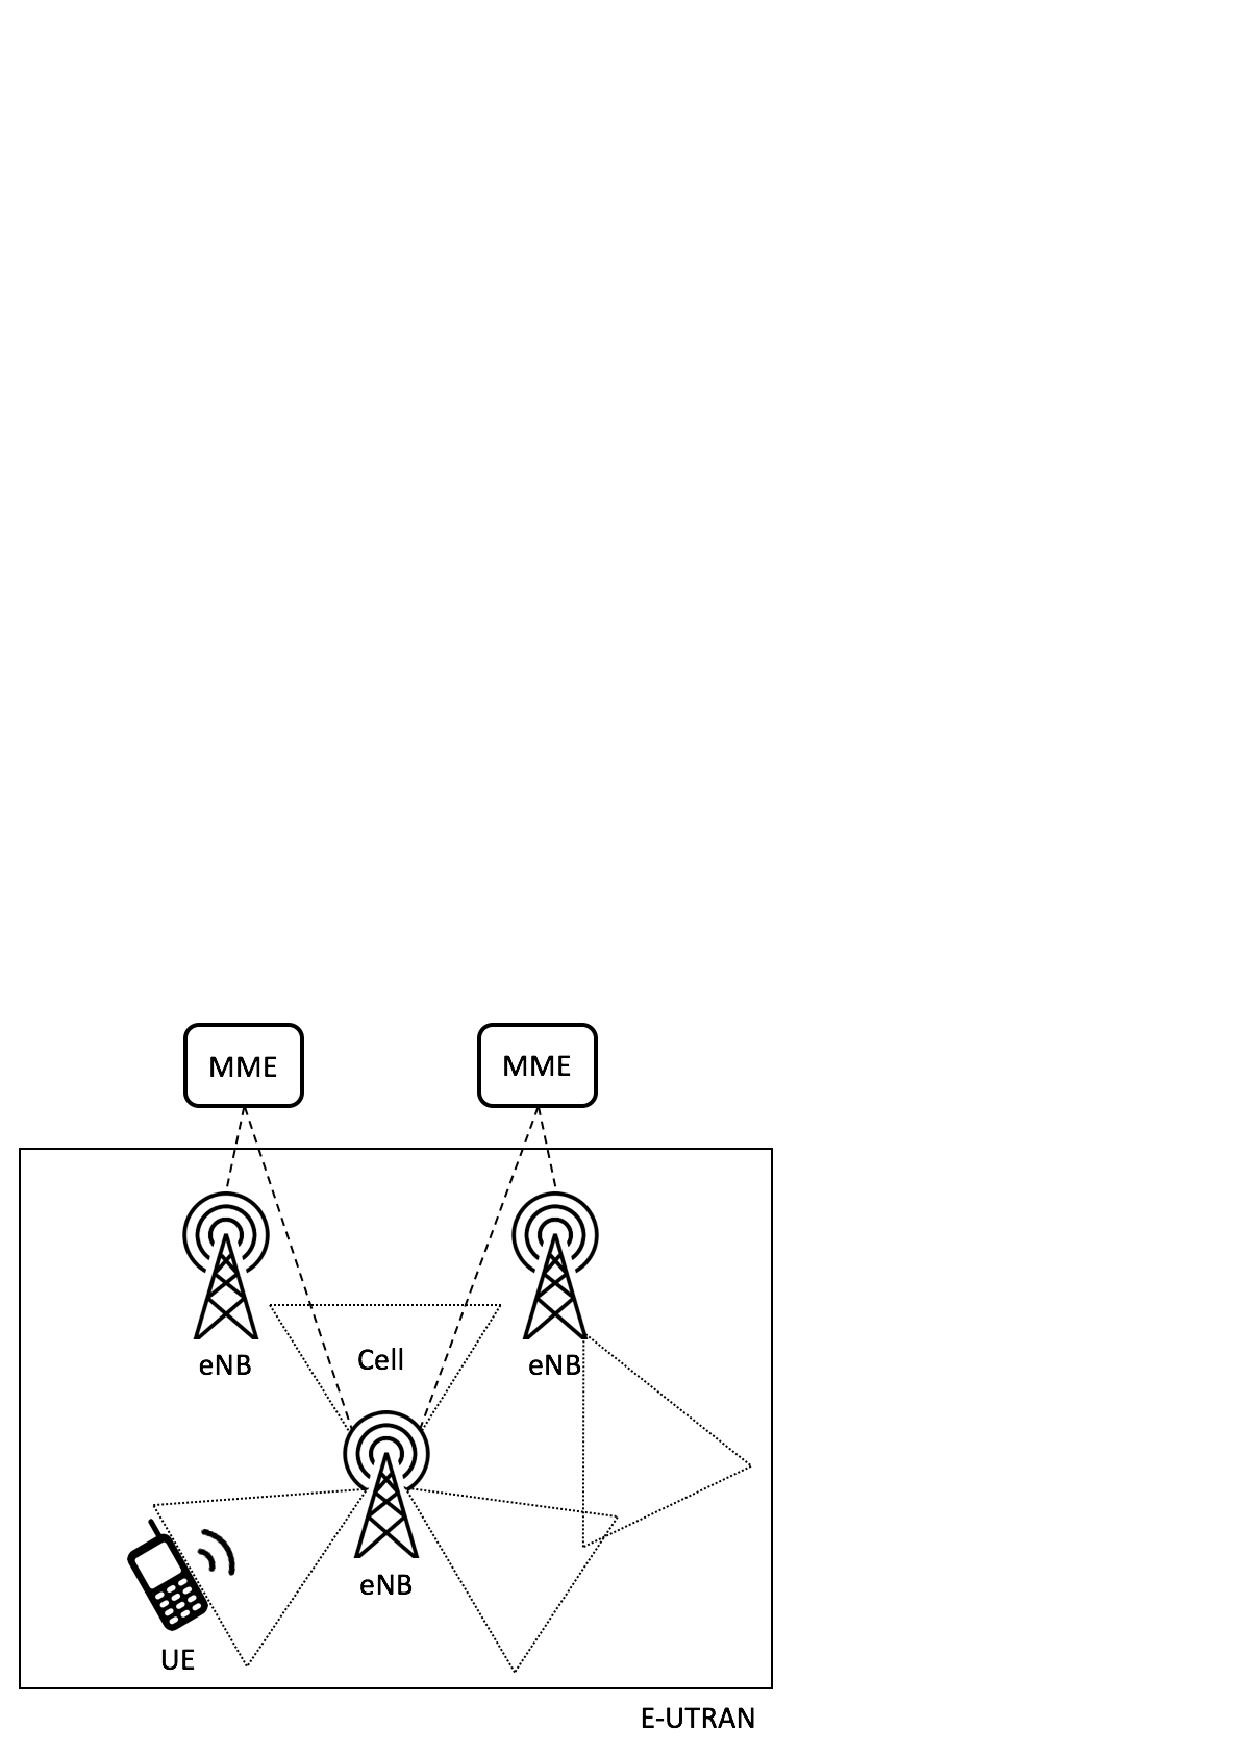
\includegraphics[scale=0.55]{picture/LTE.PNG}
\par\end{centering}
\caption{LTE architecture overview}
\label{lte}
\end{figure}

LTE, widely known as 4G, is a radio access technology for wireless
cellular communications. The high-level network architecture of LTE
is shown in \ref{lte} and is described as follows \citep{dahlman20134g}.
The E-UTRAN, an official standard name for the radio access network
of LTE, is the entire radio access network. It handles the radio communication
between the User Equipment (UE) or mobile device and the base stations
called eNB. Each base station controls and manages radio communications
with multiple devices in one or more cells. Several base stations
are connected to a Mobility Management Entity (MME), which is a control-node
for the LTE network.%
\begin{comment}
which handles the high-level operation of the mobile for different
UEs
\end{comment}
{} MME establishes a connection and runs a security application to ensure
that the UE is allowed on the network. In LTE mobile network, multiple
UEs are connected to a single base station. A new UE performs a cell
search procedure by searching for an available eNB when it first connects
to the network. Then, the UE sends information about itself to establish
a link between the UE and the eNB. 

Network procedures that will be briefly described here are \emph{Paging}
and \emph{Handover}. Paging is used for the network setup when UE
is in an idle mode. If MME wants to notify UE about incoming connection
requests, MME will send paging messages to each eNB with cells belonging
to the Tracking Area (TA) where the UE is registered. UE will wake
up if it gets the Paging message and will react by triggering a RRC
connection request message. The paging process happens in number of
paging per second.%
\begin{comment}
The UE can enter the idle mode in order to conserve battery power.
\end{comment}
{} Handover is a process of changing the serving cells or transferring
an ongoing call from one cell to another. For instance, if the UE
begins to go outside the range of the cell and enters the area covered
by another cell, the call will be transferred to the new cell in order
to avoid the call termination. The rate of handover is in second.
\begin{comment}
(from Bro) UEs in an idle state are expected to conserve battery as
efficient as possible. Therefore, in order to achieve that goal, paging
is needed for a network setup. If MME want to notify each eNB with
cells in UE for an incoming request, MME must sends Paging messages
to wake UE up.
\end{comment}

Ericsson makes a global \emph{software release} in roughly 6-month
cycles or two major releases per year. Each of these releases contains
a bundle of features and functionality that is intended for all the
customers. The software release is labeled with \emph{L} followed
by a number related to the year of release and a letter either \emph{A}
or \emph{B,} which generally corresponds to the $1^{st}$ and $2^{nd}$
half of that year. Ericsson opens up a track for each software release
and begins a code integration track. This track becomes the main track
of the work or the focal branch for all code deliveries. There are
hundreds of teams producing code, and each team commit the code to
this track continuously. In order to create a structure for this contribution,
a daily \emph{software package} is built which can be seen as a snapshot
or a marker in the continuous delivery timeline. This software package
is then run through various automated test loops to ensure that there
are no faults in the system. The software packages are named \emph{R,}
and followed by one or more numbers, which is then followed by one
or more letters. \emph{R} stands for Release-state. To summarize,
each software package is a snapshot in the code integration timeline.
\ref{release} presents a relationship between a software release
and software packages. 

\begin{figure}[H]
\begin{centering}
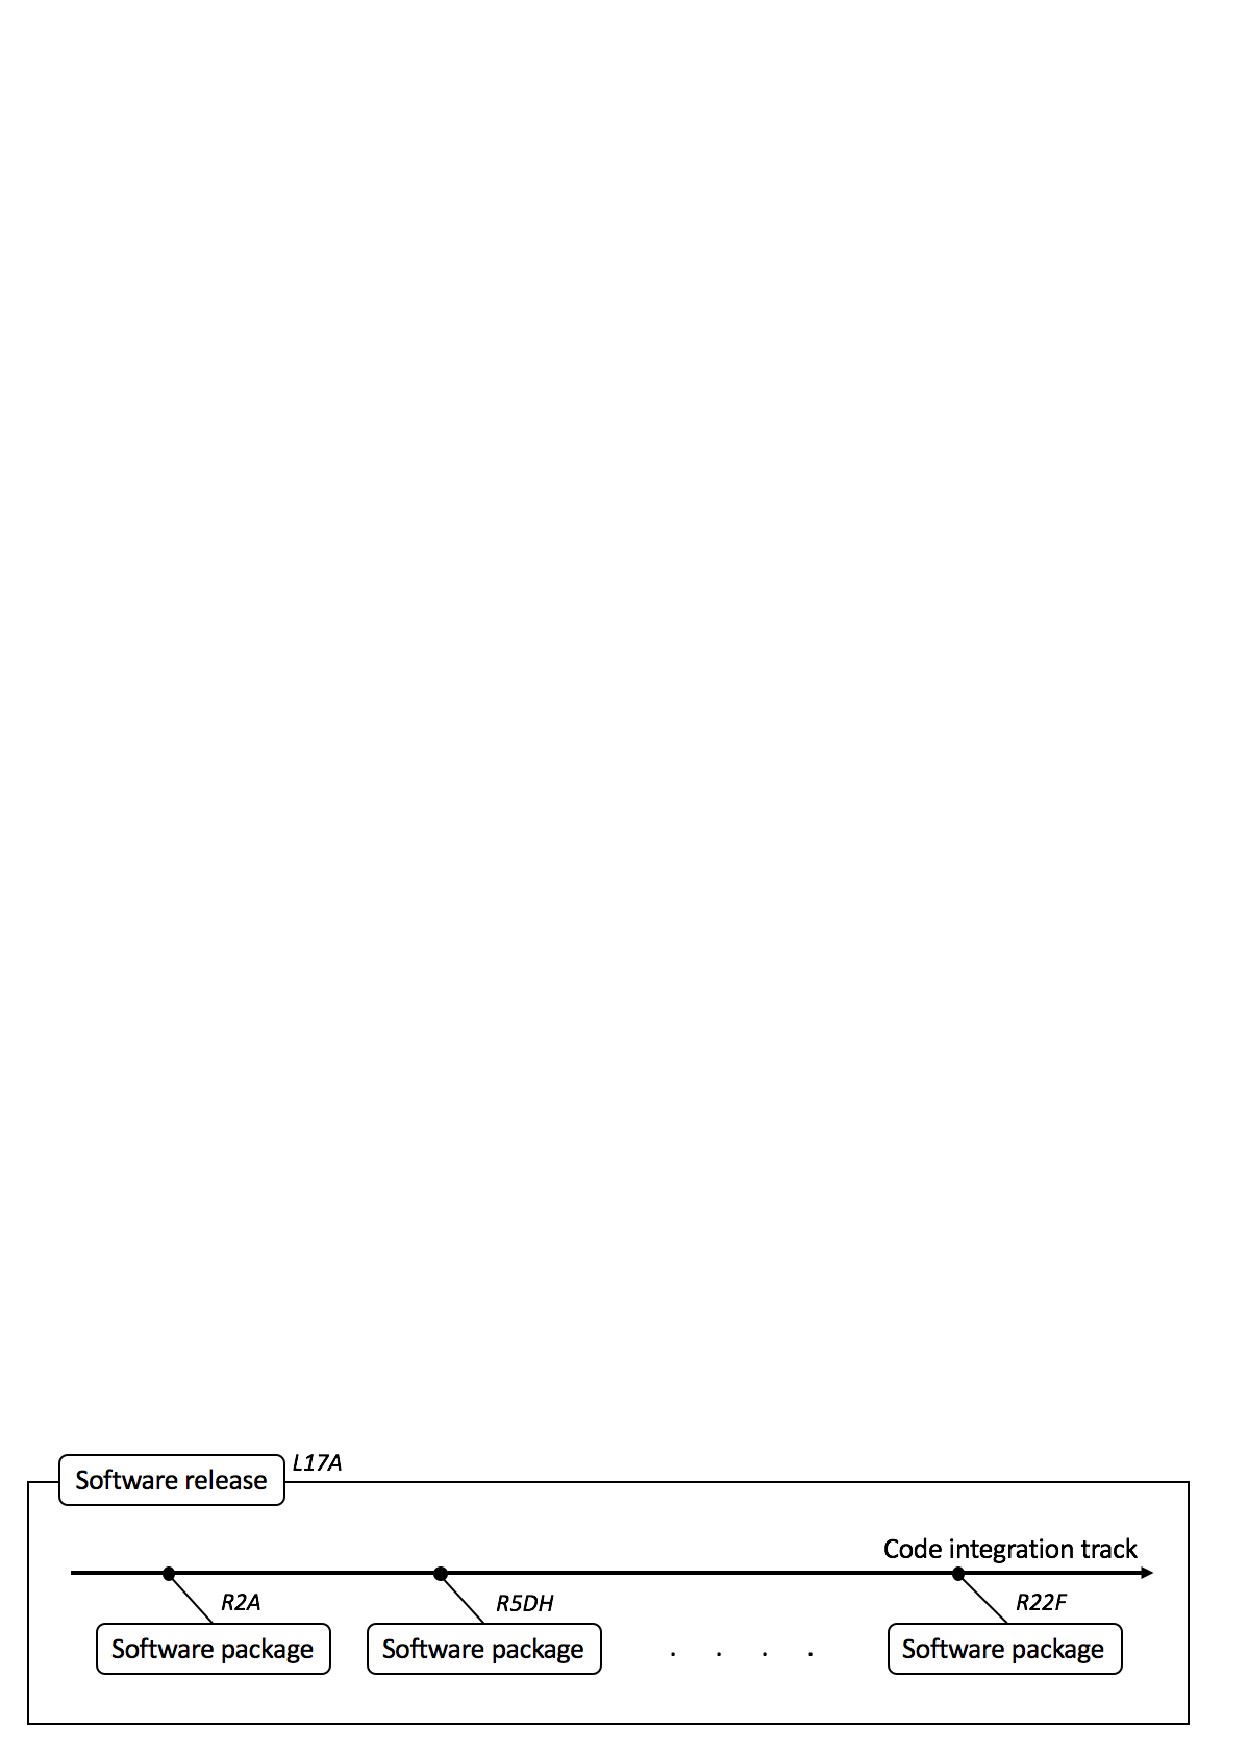
\includegraphics[scale=0.55]{picture/Release.PNG}
\par\end{centering}
\caption{An example of one software release that begins a code integration
track. Several software packages are launched in the timeline.}
\label{release}
\end{figure}

There are thousands of automated tests performed. Each test belongs
to a particular suite of tests, which belong to a particular Quality
Assurance (QA) area. For this thesis, only a subset of test cases
belonging to QA Capacity area, that focus on signaling capacity, is
used. The QA Capacity is responsible for testing and tracking test
cases related to eNB capacity. Each one of these test cases has a
well-defined traffic model that it tries to execute. The traffic model,
in this context, means certain intensity (per second) of procedures
which can be seen as stimuli in the eNB. Basically simulating the
signaling load from a large number of UEs served simultaneously by
the eNB. The eNB then increments one or more counters for each one
of these procedures or stimuli that it detects. These counters are
called local events and represented by \emph{EventsPerSec}. 

A logging loop is started during the execution of these test cases
of QA Capacity \textendash{} signaling capacity. The logging loop
collects several metrics, and a subset of these metrics is what this
thesis is currently studying. Once the logging loop is finished, it
is written to a log file. Then, there are cron jobs that slowly scan
through this infrastructure once a day to find latest logs and do
a post-processing. The final output is either CSV data or JSON encoded
charts. The flowchart of this process is illustrated in \ref{sw}.

\begin{figure}[H]
\begin{centering}
\includegraphics[scale=0.7]{picture/SW.PNG}
\par\end{centering}
\caption{An example of one software package. First, QA Capacity automated test
suites is started. For each test suite, a logging loop is started
and a log is produced for each test case. The log file is fed to post-processing
tools, and the data output is obtained.}
\label{sw}
\end{figure}


\section{Data description}

The data used in the thesis%
\begin{comment}
for the second generation (\emph{G2}) product which
\end{comment}
{} contains 2,781 test cases. It is collected on 20 January 2017 and
is extracted from log files produced by test cases. There are different
types of test cases which are being executed in the automated test
suites. Each test case is viewed as an observation in the data. The
following are the variables in the data:

\paragraph{Metadata of test case}
\begin{itemize}
\item Timestamp: Date and time when a test case is being executed (yy-dd-mm
hh:mm:ss) 
\item NodeName: IP address or the name of a base station
\item DuProdName: Product hardware name
\item Fdd/Tdd: Different standard of LTE 4G Technology. FDD and TDD stand
for Frequency Division Duplex and Time Division Duplex, respectively.
\item NumCells: Number of cells in the base station
\item Release: Software release 
\item SW: Software package
\item LogFilePath: Path for log file produced by a test case
\end{itemize}

\paragraph{Observable memory}
\begin{itemize}
\item MemFreeKiB
\item SwapFreeKiB
\item BufferCacheKiB
\item PageCacheKiB
\item RealFreeKiB
\end{itemize}

\paragraph{CPU}
\begin{itemize}
\item TotCpu\%%
\begin{comment}
: Performance of a test case in terms of CPU utilization
\end{comment}
\item PerCpu\%
\item PerThread\%
\item EventsPerSec 

The EventsPerSec variable, or Event intensity, contains several local
events that can be used when defining the test cases. Apparently,
there is no fixed number of local events in this variable as different
test cases involve different testing procedures. The local events
along with their values are also varied depending on which types of
test cases are being executed. An example of the local events in test
cases is shown in \ref{eventspersec}.

\begin{table}[H]
\caption{List of local events in the test cases separated by a tab character}
\label{eventspersec}
\centering{}%
\begin{tabular}{|c|>{\centering}p{11cm}|}
\hline 
Test case & EventsPerSec\tabularnewline
\hline 
\hline 
1 & ErabDrbRelease=166.11 ErabSetupInfo=166.19 PerBbUeEventTa=167.98 PerBbUetrCellEvent=12.00
ProcInitialCtxtSetup=166.20 RrcConnSetupAttempt=166.21 RrcConnectionRelease=166.11
S1InitialUeMessage=166.20 UplinkNasTransport=32.06

...\tabularnewline
\hline 
2 & ErabDrbAllocated=641.30 EventS1InitialUeMessage=142.20 McRrcConnectionRequest=142.99
McX2HandoverRequest=98.70 Paging=1399.94 PerBbLcgEvent=26.14

...\tabularnewline
\hline 
... & ...\tabularnewline
\hline 
\end{tabular}
\end{table}

\end{itemize}

\section{Data preprocessing}

The relevant aspects of the data preprocessing step is describe here.
The dataset, which spans three software releases \textendash{} L16A,
L16B and L17A, is split into three datasets according to the software
release. The test cases in each dataset are sorted by its software
package version, which is named alphabetically. The name of the software
package is used as a time point in the time series.

Some test cases are filtered out in the preprocessing step because
the test cases are not always executed properly. The problem is either
no traffic is generated during the test case or the data is not logged.
This usually result in a missing value in the \emph{EventPerSec} field,
which causes the test case to be incomplete. The particular test case
and all the data related to the test case is ignored. If the value
in any other fields is missing, the test case will also be ignored. 

In \ref{eventspersec}, it can be seen that the \emph{EventsPerSec}
stores multiple values separated by a tab character. These tab-separated
values in the field are split into columns. Further detail is described
in \ref{sec:EventsPerSec}. The process is done in order to turn its
local events and values, which characterize the test case, into usable
parameters. These parameters are later on used as predictor variables
when the Markov switching model is applied.

Each software release consists of several software packages. For each
specific software package, numerous test cases are executed. Since
a software package acts as a time point in the time series, the result
is rather difficult to visualize using every executed test case for
each software package. Hence, the test case that has the lowest value
of the CPU utilization (or minimum value of \emph{TotCpu\%}) is selected
to represent a performance of the specific software package. Although
taking an average of multiple runs for test cases in the software
package appears to be a good approach, it does not yield the best
outcome in this case. The first reason is that manipulating data can
easily be misleading. Another important reason for not using the average
value of the CPU utilization is that the essential information in
the test case could be lost. Each test case has its own local events
in \emph{EventsPerSec} field that is used for identifying the test
case. The details of these local events will be absent if the CPU
utilization of the test case is averaged. It is, therefore, settled
to keep the original data and always use the unmanipulated data to
visualize the time series.

\begin{comment}
The reason for choosing the minimum value of the CPU utilization is
because 

tried to be optimistic... ?
\end{comment}

After performing all the steps described above, the dataset of the
software release L16A, L16B and L17A consist of 64, 241, and 144 test
cases, respectively. Lastly, each dataset with particular software
release is divided into two subsets. Ninety percents of the dataset
is used for training the model and the remaining ten percents is left
out for testing the model 

Some variables in the data are chosen to be used for further analysis.
In total, there are one response variable and six predictor variables.
\ref{data} shows the name of variables and their descriptions. The
first three predictor variables are local events of the test case,
which can be found in the \emph{EventsPerSec}, while the last three
variables are considered as the test environment. These variables
appear to have a high influence to the CPU utilization.

\begin{table}[H]
\caption{List of the selected variables followed by its type and unit measure }
\label{data}
\centering{}%
\begin{tabular}{|l||l|l|l|}
\hline 
Variable & Name & Type & Unit\tabularnewline
\hline 
\hline 
Response  & TotCpu\% & Continuous & Percentage\tabularnewline
\hline 
Predictor  & RrcConnectionSetupComplete & Continuous & Per second\tabularnewline
 & Paging & Continuous & Per second\tabularnewline
 & X2HandoverRequest & Continuous & Per second\tabularnewline
 & DuProdName & Categorical & \tabularnewline
 & Fdd/Tdd & Binary & \tabularnewline
 & NumCells & Categorical & \tabularnewline
\hline 
\end{tabular}
\end{table}





\lhead[\chaptername~\thechapter]{\rightmark}

\rhead[\leftmark]{}

\lfoot[\thepage]{}

\cfoot{}

\rfoot[]{\thepage}

\chapter{Methods}

This chapter first starts by providing a survey of existing methods
that address the problem of detecting changes in a system. Later on,
general information about Markov chains, the simple Markov switching
model feature, and model specification namely Markov switching autoregressive
model are discussed. Thereafter, three sections are devoted to methods
for estimating the values of parameters, predicting a state for a
new observation, and selecting a suitable model for the datasets.
Another change-point method in a non-parametric approach is described.
Finally, the simulation technique is explained.

\section{Survey of existing methods}

\emph{Change point detection, Anomaly detection, Intrusion detection,
}or \emph{Outlier detection} are terms that are closely related to
one another. The main idea of these terms is to identify and discover
events that are abnormal from the usual behavior. There are several
methods to address these types of problem. A survey of existing methods
has been done in the thesis, and some methods are presented in this
section.

\citet{valdes2000adaptive} employed a Bayesian inference technique,
specifically a naive Bayesian network, to create an intrusion detection
system on traffic bursts. Even though the Bayesian network is effective
in detecting anomalies in some applications, there are some limitations
that should be considered when using this method. As accuracy of a
detection system depends heavily on certain assumptions, the system
will have low accuracy if an inaccurate model is implemented \citep{patcha2007overview}.

Support vector machine (SVM) introduced in \citet{cortes1995support}
is a supervised learning algorithm to deal with a classification analysis
problem by using the idea of separating hyperplanes. The main reason
that SVM is used in anomaly detection is because of its speed and
scalability \citep{sung2003identifying}. Although this method is
effective in identifying new kinds of anomalies, the method often
has a higher rate of false alarms due to the fact that the SVM method
ignores the relationships and dependencies between the features \citep{sarasamma2005hierarchical}. 

Self-organizing maps (SOM) developed by \citet{kohonen1982self} is
a well-known unsupervised neural network approach for cluster analysis.
SOM is efficient in handling large and high dimensional datasets.
\citet{nousiainen2009anomaly} used SOM for an anomaly detection in
a server log data. The study presented an ability of the SOM method
in detecting anomalies in the data, and also compared the results
from the SOM method with a threshold based system. A disadvantage
of the SOM is that initial weight vector affects a performance of
the SOM, which leads to an unstable clustering result. Besides, if
the anomalies in the data tend to form clusters, this method will
not be able to detect these anomalies \citep{chandola2009anomaly}. 

Based on previous works, the Hidden Markov model or the Markov switching
model has also been used in identifying changes and anomalies. One
drawback from the method based on the Markov chain is that the method
has a high computational cost, which is not scalable for an online
change application \citep{patcha2007overview}. Apart from changes
that can be detected in the data, some knowledge about the unobservable
condition of the system can also be obtained. This additional information
makes the method more appealing than the other methods. Therefore,
the Markov switching model is implemented in this thesis framework. 

\section{Technical aspects}

The thesis work has been carried out using the \emph{R} programming
language \citep{rprogram} for the purpose of data cleaning, preprocessing,
and analysis. The Markov switching model was performed using the \emph{MSwM}
package. Various extensions and modifications were further implemented
in the package e.g., handling predictor categorical variables, the
state prediction function, and plots for visualizing the results (More
details can be found in \ref{sec:MSwM-Package}). For the E-divisive
method, the \emph{ecp} package was used. 

\section{Markov chains\label{sec:Markov-chains}}

A Markov chain is a random process which has a property that is given
the current value, the future is independent of the past. A random
process $X$ contains random variables $X_{t}:\:t\in T$ indexed by
a set $T$. When $T=\{0,1,2,...\}$ the process is called a discrete-time
process, and when $T=[0,\infty)$ it is called a continuous-time process.
Let $X_{t}$ be a sequence of values from a state space $S$. The
process begins from one of these states and moves to another state.
The move between states is called a step. The process of Markov chains
is described here.
\begin{defn}
\citep[p.214]{grimmett2001probability} If a process $X$ satisfies
the Markov property, the process $X$ is a first order Markov chain

\[
P(X_{t}=s|X_{0}=x_{0},X_{1}=x_{1},...,X_{t-1}=x_{t-1})=P(X_{t}=s|X_{t-1}=x_{t-1})
\]

where $t\ge1$ and $s,x_{0},...,x_{t-1}\in S$
\end{defn}
If $X_{t}=i$ then the chain is in state $i$ or the chain is in the
$i$th state at the $t$th step. 

There are transitions between states which describe the distribution
of the next state given the current state. The evolution of changing
from $X_{t}=i$ to $X_{t}=j$ is defined as the transition probability
$P(X_{t}=j|X_{t-1}=i)$. For Markov chains, it is frequently assumed
that these probabilities depend only on $i$ and $j$ and do not depend
on $t$.
\begin{defn}
\citep[p.214]{grimmett2001probability} A Markov chain is \emph{time-homogeneous}
if

\[
P(X_{t+1}=j|X_{t}=i)=P(X_{1}=j|X_{0}=i)
\]

for all $t,i,j$. The probability of the transition is independent
of $t$. A \emph{transition matrix} $\mathbf{P}=(p_{ij})$ is a matrix
of transition probabilities 

\[
p_{ij}=P(X_{t}=j|X_{t-1}=i)\qquad\mathrm{for}\,\mathrm{all\,}t,i,j
\]
\end{defn}
\begin{thm*}
\citep[p.215]{grimmett2001probability} The transition matrix $\mathbf{P}$
is a matrix that
\begin{itemize}
\item Each of the entries is a non-negative real number or $p_{ij}\ge0$
for all $i,j$
\item The sum of each row equal to one or $\sum_{j}p_{ij}=1$ for all $i$
\end{itemize}
\end{thm*}

\begin{defn}
\label{def:-The-vector}\citep[p.227]{grimmett2001probability} The
vector $\pi$ is called a \emph{stationary distribution} if $\pi$
has entries $(\pi_{j}:\:j\in S)$ that satisfies
\begin{itemize}
\item $\pi_{j}\geq0$ for all $j$, and $\sum_{j}\pi_{j}=1$
\item $\pi=\pi\mathbf{P}$, which is $\pi_{j}=\sum_{i}\pi_{i}p_{ij}$ for
all $j$
\end{itemize}
\end{defn}

\begin{defn}
\citep[p.220]{grimmett2001probability} A state $i$ is called persistent
(or recurrent) if

\[
P(X_{t}=i\mathrm{\:for\,}\mathrm{some\,\mathrm{t}}\geq1|X_{0}=i)=1
\]
\end{defn}

Let $f_{ij}(t)=P(X_{1}\neq j,X_{2}\neq j,...,X_{t}=j|X_{0}=i)$ be
the probability of visiting state $j$ first by starting from $i$,
takes place at $t$th step.

\begin{defn}
\citep[p.222]{grimmett2001probability} The mean recurrence time of
a persistent state $i$ is defined as

\[
\mu_{i}=E(T_{i}|X_{0}=i)=\sum_{n}n\cdot f_{ii}(n)
\]

A persistent state $i$ is non-null (or positive recurrent) if $\mu_{i}$
is finite. Otherwise, the persistent state $i$ is null. 
\end{defn}

\begin{defn}
\citep[p.222]{grimmett2001probability} The period $d(i)$ of a state
$i$ is defined as 

\[
d(i)=gcd\{n:\:p_{ii}(n)>0\}
\]

where $gcd$ is the greatest common divisor. If $d(i)=1$, then the
state is said to be aperiodic. Otherwise, the state is said to be
periodic. 
\end{defn}

\begin{defn}
\citep[p.222]{grimmett2001probability} A state is called ergodic
if it is non-null persistent and aperiodic.
\end{defn}

\begin{defn}
A chain is called irreducible if it is possible to go from every state
to every other states.
\end{defn}

\begin{thm*}
If all states in an irreducible Markov chain are ergodic, the chain
is said to be ergodic.
\end{thm*}

\begin{thm*}
\citep{manning2008introduction} If there is an aperiodic finite state,
an irreducible Markov chain is the same thing as an ergodic Markov
chain. 
\end{thm*}

\section{Markov switching model}

A Markov switching model is a switching model where the shifting back
and forth between the states or regimes is controlled by a latent
Markov chain. The model structure consists of two stochastic processes
embedded in two levels of hierarchy. One process is an underlying
stochastic process that is not normally observable, but possible to
be observed through another stochastic process which generates the
sequence of observation \citep{rabiner1986introduction}. The transition
time between two states is random. In addition, the state are assumed
to follow the Markov property that the future state depends only on
the current state. 

The Markov switching model is able to model more complex stochastic
processes and describe changes in the dynamic behavior. A general
structure of the model can be drawn graphically as shown in \ref{msm},
where $S_{t}$ and $y_{t}$ denote the state sequence and observation
sequence in the Markov process, respectively. The arrows from one
state to another state in the diagram implies a conditional dependency. 

\begin{figure}[H]
\begin{centering}
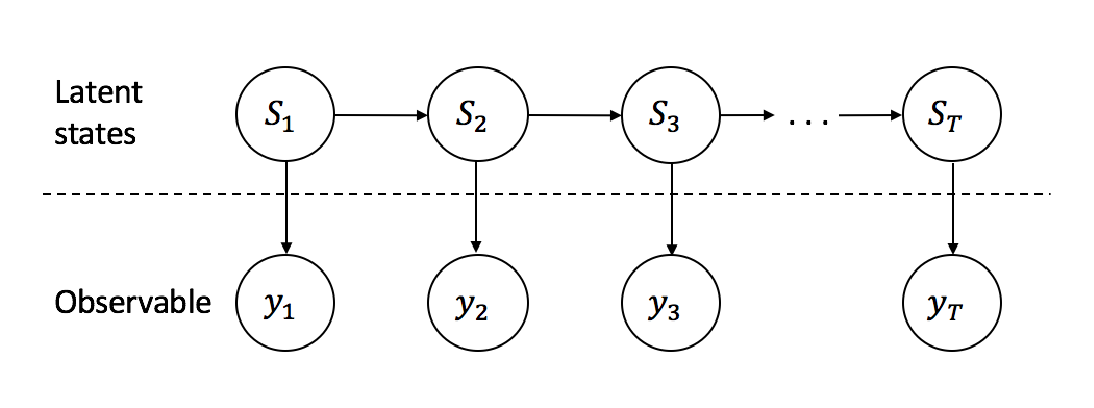
\includegraphics[scale=0.6]{picture/msm1}
\par\end{centering}
\caption{Model structure}
\label{msm}
\end{figure}

The process is given by \citep{hamilton1989new}

\begin{equation}
y_{t}=X_{t}\beta_{S_{t}}+\varepsilon_{t}\label{eq:general_mswm}
\end{equation}
where, 
\begin{labeling}{00.00.0000}
\item [{$y_{t}$}] is an observed value of the time series at time $t$
\item [{$X_{t}$}] is a design matrix, also known as model matrix, containing
values of predictor variables of the time series at time $t$
\item [{$\beta_{S_{t}}$}] are a column vector of coefficients in state
$S_{t}$, where $S_{t}\in\{1,...,k\}$ 
\item [{$\varepsilon_{t}$}] follows a normal distribution with zero mean
and variance given by $\sigma_{S_{t}}^{2}$ 
\end{labeling}
Equation \ref{eq:general_mswm} is the simplest form for the switching
model. To aid understanding, the baseline model is assumed to have
only two states $(k=2)$ in this discussion. $S_{t}$ is a random
variable which is assumed that the value $S_{t}=1$ for $t=1,2,...,t_{0}$
and $S_{t}=2$ for $t=t_{0}+1,t_{0}+2,...,T$ where $t_{0}$ is a
known change point. 

The transition matrix $\mathbf{P}$ is an $2\mathrm{x}2$ matrix where
row $j$ column $i$ element is the transition probability $p_{ij}$.
A diagram showing a state-transition is shown in \ref{transition}.
Note that these probabilities are independent of $t$.

\begin{figure}[H]
\begin{centering}
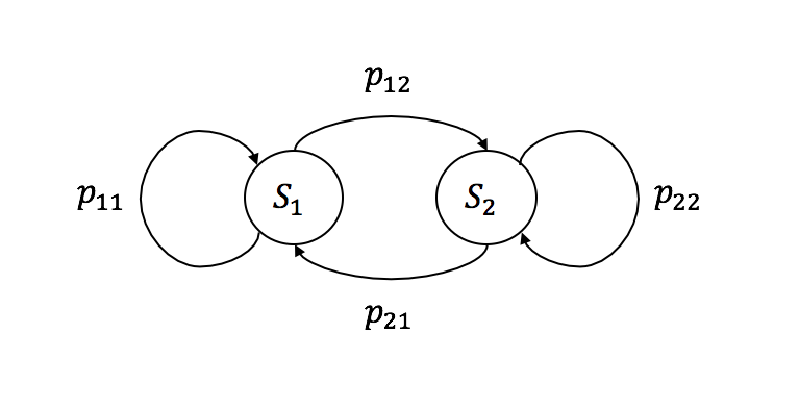
\includegraphics[scale=0.6]{picture/transition}
\par\end{centering}
\caption{State-transition diagram}
\label{transition}
\end{figure}

Since the whole process $S_{t}$ is unobserved, the initial state
where $t=0$ also needs to be specified. The probability which describes
the starting distribution over states is denoted by

\[
\pi_{i}=P(S_{0}=i)
\]

There are several options for computing the probability of the initial
state. One procedure is to commonly set $P(S_{0}=i)=0.5$. Alternatively,
by presuming an ergodic Markov chain \citep{hamilton2005regime},
a stationary distribution is 

\[
\pi_{i}=P(S_{0}=i)=\frac{1-p_{jj}}{2-p_{ii}-p_{jj}}
\]

which is simply from solving the system of equations $\pi=\pi\mathbf{P}$. 
\begin{proof}
Let $\pi=(\pi_{1},\pi_{2})'$ and $\mathbf{P}=\left[\begin{array}{cc}
p_{ii} & 1-p_{ii}\\
1-p_{jj} & p_{jj}
\end{array}\right]$

Definition\ref{def:-The-vector} of a stationary distribution, 
\begin{eqnarray}
\pi & = & \pi\mathbf{P}\label{eq:1}
\end{eqnarray}
and
\begin{eqnarray}
\pi_{1}+\pi_{2} & = & 1\label{eq:2}
\end{eqnarray}
From \ref{eq:1},
\begin{eqnarray*}
\pi_{1} & = & \pi_{1}p_{ii}+\pi_{2}(1-p_{jj})\\
\pi_{2} & = & \pi_{1}(1-p_{ii})+\pi_{2}p_{jj}
\end{eqnarray*}
Therefore,
\begin{eqnarray}
\pi_{2} & = & \frac{\pi_{1}(1-p_{ii})}{1-p_{jj}}\label{eq:3}
\end{eqnarray}

Substitute \ref{eq:3} into Equation \ref{eq:2}, then
\begin{eqnarray*}
\pi_{1} & = & \frac{1-p_{jj}}{2-p_{ii}-p_{jj}}
\end{eqnarray*}
\end{proof}
A coefficient of a predictor variable in the Markov switching model
can have either different values in different state or a constant
value in all state. The variable which have the former behavior is
said to have a \emph{switching effect}. Likewise, the variable which
have the same coefficient in all states is the variable that does
not have a switching effect, or said to have a \emph{non-switching
effect.} 

A generalized form of Equation \ref{eq:general_mswm} can be defined
as \citep{perlin2015ms_regress}

\begin{equation}
y_{t}=X_{t}^{ns}\alpha_{t}+X_{t}^{s}\beta_{S_{t}}+\varepsilon_{t}
\end{equation}

where, 
\begin{labeling}{00.00.0000}
\item [{$X_{t}^{ns}$}] contains all predictor variables that have non-switching
effect of the time series at time $t$
\item [{$\alpha_{t}$}] are non-switching coefficients of the time series
at time $t$
\item [{$X_{t}^{s}$}] contains all predictor variables that have the switching
effect of the time series at time $t$
\item [{$\beta_{S_{t}}$}] are switching coefficients in state $S_{t}$,
where $S_{t}\in\{1,...,k\}$
\item [{$\varepsilon_{t}$}] follows a normal distribution with zero mean
and variance given by $\sigma_{S_{t}}^{2}$ 
\end{labeling}

\subsection{Autoregressive (AR) model}

An autoregressive model is one type of time series models used to
describe a time-varying process. The model is flexible in handling
various kinds of time series patterns. The name autoregressive comes
from how the model performs a regression of the variable against its
own previous outputs \citep{cryer1986time}. The number of autoregressive
lags (i.e., the number of prior values used in the model) is denoted
by $p$. 
\begin{defn}
An autoregressive model of order $p$ or AR(p) model can be written
as 

\[
y_{t}=c+\sum_{i=1}^{p}\phi_{i}y_{t-i}+\varepsilon_{t}
\]

where $c$ is a constant, $\phi_{i}$ are coefficients in the autoregression
and $\varepsilon_{t}$ follows a normal distribution with zero mean
and variance $\sigma^{2}$.
\end{defn}
If $p$ is equal to one, the model AR(1) is called the first order
autoregression process.

\subsection{Markov switching autoregressive model}

A Markov switching autoregressive model is an extension of a basic
Markov switching model where observations are drawn from an autoregressive
process. The model relaxes the conditional independence assumption
by allowing an observation to depend on both past observation and
a current state \citep{shannon2009formulation}. Basically, this is
the combination between the Markov switching model and the autoregressive
model.
\begin{defn}
The first order Markov switching autoregressive model is 

\[
y_{t}=X_{t}\beta_{S_{t}}+\phi_{1,S_{t}}y_{t-1}+\varepsilon_{t}
\]

where $\phi_{1,S_{t}}$ is an autoregressive coefficient of the observed
value at time $t-1$ in state $S_{t}$. $\varepsilon_{t}$ follows
a normal distribution with zero mean and variance given by $\sigma_{S_{t}}^{2}$.
\end{defn}
The structure of the model is shown in \ref{msm-ar}. It can be clearly
seen that there is a dependency at the observation level.

\begin{figure}[H]
\begin{centering}
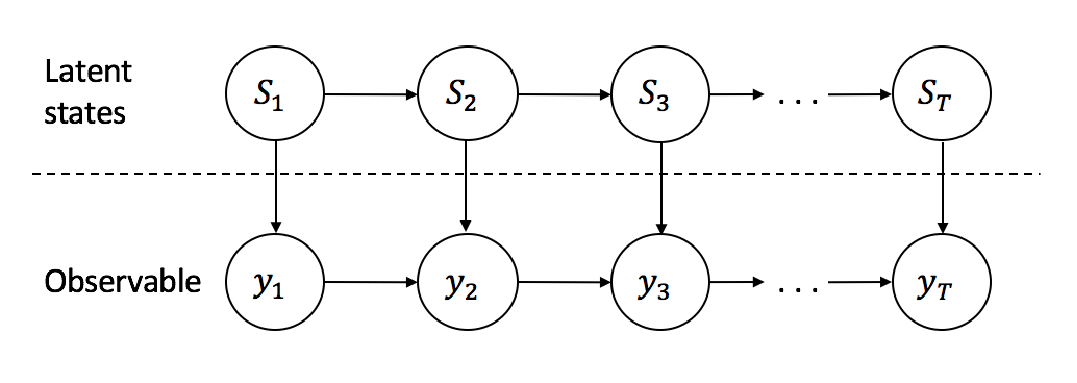
\includegraphics[scale=0.6]{picture/msm-ar1}
\par\end{centering}
\caption{Model structure of Markov switching AR(1)}
\label{msm-ar}
\end{figure}

Assuming two states $S_{t}=1$ or $2$, the set of parameters that
are necessary to describe the law of probability that governs $y_{t}$
are $\theta=\{\beta_{1},\beta_{2},\phi_{1,1},\phi_{1,2},\sigma_{1}^{2},\sigma_{2}^{2},\pi_{1},\pi_{2},p_{11},p_{22}\}$. 

For the simplicity, in this thesis, the term Markov switching autoregressive
model will be addressed as the Markov switching model.

\section{Parameter estimation}

There are various ways to estimate parameters of a Markov switching
model. Methods which have been widely used are as follows: E-M algorithm
\citep{hamilton1990analysis,kim1994dynamic} uses the maximum likelihood
criterion, Segmental K-means \citep{juang1990segmental} uses K-means
algorithm and maximizes the state-optimized likelihood criterion,
and Gibbs sampling \citep{kim1999state} uses a Markov chain Monte
Carlo simulation method based on the Bayesian inference. 

In this thesis framework, the E-M algorithm is used in estimating
parameters as the algorithm gives effective results, numerically stable,
and easy to implement. \citet{ryden2008versus} compared the computational
perspective in estimating parameters between the E-M algorithm and
the Gibbs sampling. In most cases, the Gibbs sampling tended to have
less computational time than the E-M algorithm. However, the study
indicated that if the number of states was unknown and only point
estimate was sufficient, the E-M algorithm would typically be simpler
and quicker solution in computing the estimated parameters. The E-M
algorithm is briefly described below. %
\begin{comment}
Summing up this case, we first remark that if one wants to compute
only the best model without any further information on how plausible
it is relative to other ones, then the simplest solution is using
EM to compute MLEs for all candidate models and then calculating and
comparing their BICs or some other penalized likelihood criterion.
\end{comment}


\subsection{The Expectation-Maximization algorithm}

E-M algorithm is originally designed to deal with the problem of incomplete
or missing values in data \citep{dempster1977maximum}. Nevertheless,
it could be implemented in Markov switching model since the unobserved
state $S_{t}$ can be viewed as missing data values. 

The set of parameters $\theta$ are estimated by an iterative two-step
procedure. In the first step, the algorithm starts with arbitrary
initial parameters, and then finds the expected values of the state
process from the given observations. In the second step of the iterative
procedure, a new maximum likelihood from the derived parameters in
the previous step is calculated. These two steps are repeated until
the maximum value of the likelihood function is reached or has converged
\citep{janczura2012efficient}. The two steps are known as the E-step
and the M-step. \ref{em} illustrates the process of the E-M algorithm.

\begin{figure}[H]
\begin{centering}
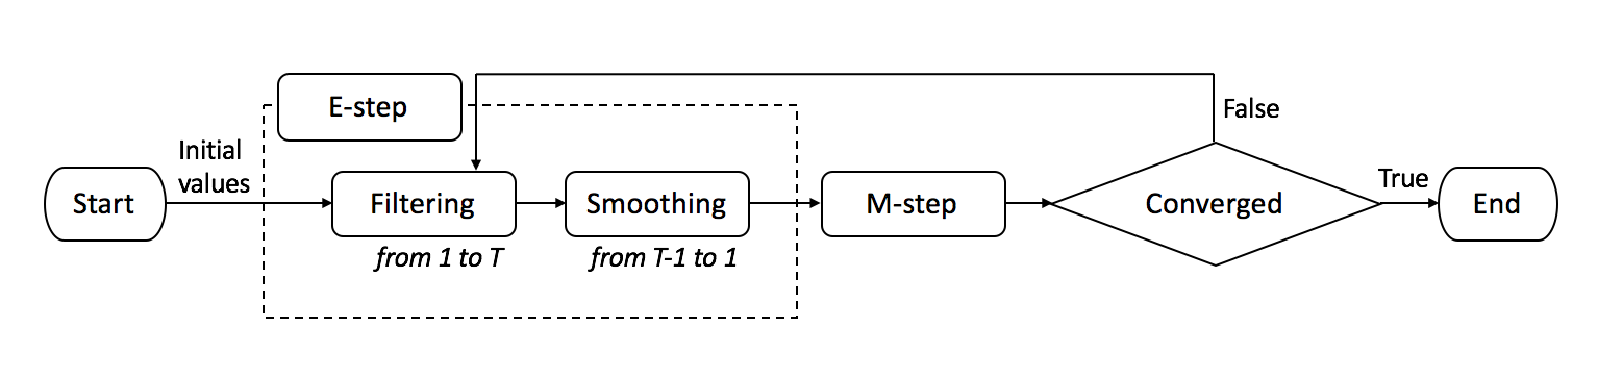
\includegraphics[scale=0.55]{picture/em}
\par\end{centering}
\caption{A flowchart showing the process of the Expectation-Maximization algorithm.
The algorithm begins with a set of initial values. The E-step is performed
by computing a filtering and smoothing algorithm. Then, the M-step
is performed. Iterating both steps until convergence.}

\label{em}
\end{figure}


\subsubsection{E-step}

In this step, $\theta^{(n)}$ is the derived set of parameters in
M-step from the previous iteration, and $n$ is a current iteration
in the algorithm. The available observations of time $t-1$ is denoted
as $\Omega_{t-1}=(y_{1},y_{2},...,y_{t-1})$. The general idea of
this step is to calculate the expectation of $S_{t}$ under the current
estimation of the parameters. The obtained result is called smoothed
inferences probability, and is denoted by $P(S_{t}=j|\Omega_{T};\theta)$
where $T$ is the number of all observations in the data and $j=1,2,...,k$.
The E-step which consists of filtering and smoothing algorithm is
described as follows \citep{kim1994dynamic}:

\paragraph{Filtering}

A filtered probability is a probability of a non-observable Markov
chain being in a given state $j$ at time $t$, conditional on information
up to time $t$. The algorithm starts from $t=1$ to $t=T$. A starting
point for the first iteration where $t=1$ is chosen from arbitrary
values. The probabilities of each state given available observations
up to time $t-1$ is calculated by

\begin{equation}
P(S_{t}=j|\Omega_{t-1};\theta^{(n)})=\sum_{i=1}^{k}p_{ij}^{(n)}P(S_{t-1}=i|\Omega_{t-1};\theta^{(n)})\qquad j=1,2,...,k
\end{equation}

The conditional densities of $y_{t}$ given $\Omega_{t-1}$ are

\begin{equation}
f(y_{t}|\Omega_{t-1};\theta^{(n)})=\sum_{j=1}^{k}f(y_{t}|S_{t}=j,\Omega_{t-1};\theta^{(n)})P(S_{t}=j|\Omega_{t-1};\theta^{(n)})
\end{equation}

where $f(y_{t}|S_{t},\Omega_{t-1};\theta)=\frac{1}{\sqrt{2\pi\sigma_{S_{t}}^{2}}}exp\left\{ -\frac{(y_{t}-\beta_{S_{t}})^{2}}{2\sigma_{S_{t}}^{2}}\right\} $
is the likelihood function in each state for time $t$. This is simply
a Gaussian probability density function.

Then, with the new observation at time $t$, the probabilities of
each state are updated by using Bayes' rule as shown below

\begin{equation}
P(S_{t}=j|\Omega_{t};\theta^{(n)})=\frac{f(y_{t}|S_{t}=j,\Omega_{t-1};\theta^{(n)})P(S_{t}=j|\Omega_{t-1};\theta^{(n)})}{f(y_{t}|\Omega_{t-1};\theta^{(n)})}\label{eq:fProb}
\end{equation}

The process above is computed iteratively until all the observation
is reached i.e., $t=T$.

\begin{comment}
The joint conditional density function of $y_{t},$$S_{t-1}$and $S_{t}$
given $\Omega_{\ensuremath{t-1}}$ are

\[
f(y_{t},S_{t-1}=i,S_{t}=j|\Omega_{t-1};\theta^{(n)})=f(y_{t}|S_{t-1}=i,S_{t=}j,\Omega_{t-1};\theta^{(n)})P(S_{t-1}=i,S_{t}=j|\Omega_{t-1};\theta^{(n)})
\]

and 

\[
P(S_{t-1}=i,S_{t}=j|\Omega_{t};\theta^{(n)})=\frac{f(y_{t},S_{t-1}=i,S_{t}=j|\Omega_{t-1};\theta^{(n)})}{f(y_{t}|\Omega_{t-1};\theta^{(n)})}
\]
\end{comment}


\paragraph{Smoothing}

A smoothed probability is a probability of a non-observable Markov
chain being in state $j$ at time $t$, conditional on all available
information. The algorithm iterates over $t=T-1,T-2,...,1$. The starting
values are obtained from the final iteration of the filtered probabilities.

By noting that

\begin{align}
P(S_{t}=j|S_{t+1}=i,\Omega_{T};\theta^{(n)}) & \thickapprox P(S_{t}=j|S_{t+1}=i,\Omega_{t};\theta^{(n)})\nonumber \\
 & =\frac{P(S_{t}=j,S_{t+1}=i|\Omega_{t};\theta^{(n)})}{P(S_{t+1}=i|\Omega_{t};\theta^{(n)})}\nonumber \\
 & =\frac{P(S_{t}=j|\Omega_{t};\theta^{(n)})p_{ij}^{(n)}}{P(S_{t+1}=i|\Omega_{t};\theta^{(n)})}
\end{align}

and

\begin{equation}
P(S_{t}=j|\Omega_{T};\theta^{(n)})=\sum_{i=1}^{k}P(S_{t}=j,S_{t+1}=i|\Omega_{T};\theta^{(n)})
\end{equation}

then, the smoothed probabilities can be expressed as

\begin{equation}
P(S_{t}=j|\Omega_{T};\theta^{(n)})=\sum_{i=1}^{k}\frac{P(S_{t+1}=i|\Omega_{T};\theta^{(n)})P(S_{t}=j|\Omega_{t};\theta^{(n)})p_{ij}^{(n)}}{P(S_{t+1}=i|\Omega_{t};\theta^{(n)})}
\end{equation}


\paragraph{Full log-likelihood}

Once the filtered probabilities are estimated, there is enough necessary
information to compute the full log-likelihood function.

\begin{equation}
\ln L(\theta)=\sum_{t=1}^{T}\ln(f(y_{t}|\Omega_{t-1};\theta^{(n)})=\sum_{t=1}^{T}\ln\sum_{j=1}^{k}((f(y_{t}|S_{t}=j,\Omega_{t-1};\theta^{(n)})P(S_{t}=j|\Omega_{t-1}))\label{eq:loglik}
\end{equation}

This is simply a weighted average of the likelihood function in each
state. The probabilities of states are considered as weights.

\subsubsection{M-step}

The new estimated model parameters $\theta^{(n+1)}$ are obtained
by finding a set of parameters that maximizes Equation \ref{eq:loglik}.
This new set of parameters is more precise than the previous estimated
value of the maximum likelihood. $\theta^{(n+1)}$ serves as a set
of parameters in the next iteration of the E-step. 

Each individual parameter in $\theta^{(n+1)}$ are taken from its
maximum value, which is determined by taking the partial derivative
of the log-likelihood function with respect to each parameter. Generally,
this process is similar to the standard maximum likelihood estimation.
However, it has to be weighted by the smoothed probabilities because
each observation $y_{t}$ contains probability from each $k$ states. 

\subsubsection{Convergence of the E-M algorithm}

The E- and M-step are iteratively computed until the algorithm converges.
The algorithm will terminate when the different between the previous
and current estimate values is less than a specific value. This specific
value called a \emph{stopping criterion} needs to be specified beforehand.
The convergence is assured since the value of the log-likelihood function
will increase in each iteration. However, the E-M algorithm does not
guarantee to always converge to a global maximum. The convergence
of the algorithm is also likely to be only a local maxima. 

\section{State prediction}

The package used for performing the Markov switching model does not
provide a function to predict the most probable state for the new
observation. Therefore, the state prediction function is implemented
as an additional function in the package for this analysis (see \ref{sec:MSwM-Package}).

The probabilities of being in state $j$ at time $T+1$ on a basis
of the current information are computed by performing the filtering
algorithm in the E-step of E-M algorithm. The filtered probabilities
are

\[
P(S_{T+1}=j|\Omega_{T+1};\theta)=\frac{f(y_{T+1}|S_{T+1}=j,\Omega_{T};\theta)P(S_{T+1}=j|\Omega_{T};\theta)}{f(y_{T+1}|\Omega_{T};\theta)}
\]

This is Equation \ref{eq:fProb} where $t=T+1$. Then, the new observation
at time $T+1$ is said to be in the state $j$ if it has the highest
probability.

\section{Model selection}

One of the most difficult tasks when modeling the Markov switching
model is to decide on the number of states \citep{rabiner1986introduction}.
The analysis will be conducted on a trial and error basis before settling
on the most appropriate size of the model. In this study, several
Markov switching models with different setting will be carried out.
First, the number of states $k$ for the model will be chosen. Then,
the number of switching coefficients in the model will be decided
based on the selected number of states. Models will be selected based
on the quality of the model. 

Model selection is a task of selecting the best model for a given
set of data. The Bayesian Information Criterion (BIC) is widely employed
in the applied literature, and proved to be useful in selecting the
model among a finite set of models (e.g., \citet{leroux1992maximum}
used BIC to select the number of states $k$). It is also known as
Schwarz Information Criterion \citep{schwarz1978estimating}. Model
which has a lower value of BIC is preferred. 

\[
\mathrm{BIC}=-2\ln(L(\hat{\theta}))+m\cdot\ln(T)
\]

where $L(\hat{\theta})$ represents the maximized value of the likelihood
function, $T$ is the number of observations, and $m$ is the number
of parameters to be estimated in the model. While including more parameters
or terms will result in a higher likelihood, it can also lead to an
overfitting. BIC attempts to reduce the risk of overfitting by taking
into account the number of parameters in the model. BIC can, therefore,
heavily penalize a complex model. 

\section{Non-parametric analysis}

A parametric analysis outperforms a non-parametric analysis if the
applied data belong to a known distribution family. However, a parametric
test does not perform well in detecting change points of an unknown
underlying distribution \citep{sharkey2014nonparametric}. Applying
a non-parametric analysis to a real-world process gives a real advantage
to the analysis. Data collected from a real-world process usually
do not have a well-defined structure, which are more suitable to be
applied with the non-parametric analysis that is not too restrictive
\citep{hawkins2010nonparametric}. For this reason, the non-parametric
analysis is implemented in order to get a rough idea of the change
point location in this thesis framework. The obtained result is also
compared with the result from using the Markov switching model.

\subsubsection*{E-divisive}

An \emph{ecp}\footnote{https://cran.r-project.org/web/packages/ecp/index.html}
is an extension package in \emph{R} which mainly focuses on computing
a non-parametric test for multiple change point analysis. This change
point method is applicable to both univariate and multivariate time
series. The fundamental idea of the package is based on the hierarchical
clustering approach \citep{james2013ecp}. 

An E-divisive method is an algorithm in the \emph{ecp} package. This
algorithm performs a divisive clustering in order to estimate change
points. The E-divisive recursively partitions a time series and estimates
a single change point at each iteration. Consequently, the new change
point is located in each iteration, which divides the time series
into different segments. The algorithm also uses a permutation test
to compute the statistical significance of an estimated change point.
The computational time of the E-divisive algorithm is $O(kT^{2})$,
where $k$ is the number of estimated change points and $T$ is the
number of observations in the time series data. More details about
the estimation is described in \citet{matteson2014nonparametric}. 

\section{Simulation study for model evaluation \label{sec:Simulation}}

The state of the CPU utilization in a real data is unknown in the
study. As a consequence, an accuracy of the Markov switching model
and the E-divisive method cannot be computed, and the comparison between
both methods can hardly be made. One possible solution to test how
effective both methods are, and to verify how well the implemented
state prediction function performs is to use a simulation technique.
The dataset that consists of two predictor variables and one response
variable with already known states is simulated. The actual models
of each state are 

\[
y_{t}=\begin{cases}
\begin{array}{c}
10+0.6X_{1,t}-0.9X{}_{2,t}+0.5y_{t-1}+\varepsilon_{t}^{(1)}\\
2+0.8X_{1,t}+0.2y_{t-1}+\varepsilon_{t}^{(2)}\\
-12+0.7X_{1,t}+0.2X{}_{2.t}-0.2y_{t-1}+\varepsilon_{t}^{(3)}
\end{array} & \begin{array}{c}
\varepsilon_{t}^{(1)}\sim N(0,1);\quad\mathrm{Normal}\\
\varepsilon_{t}^{(2)}\sim N(2,0.5);\quad\mathrm{Bad}\\
\varepsilon_{t}^{(3)}\sim N(1,1);\quad\mathrm{Good}
\end{array}\end{cases}
\]

where, 
\begin{labeling}{00.00.0000}
\item [{$y_{t}$}] is assumed to be a value of a CPU usage of the time
series at time $t$
\item [{$X_{1,t}$}] is a predictor variable generated by a uniform distribution
on $[50,200]$ of the time series at time $t$
\item [{$X_{2,t}$}] is a predictor variable generated by a uniform distribution
on $[0,50]$ of the time series at time $t$
\end{labeling}
There are two simulated datasets \textendash{} Dataset 1 and Dataset
2 \textendash{} and each of them contains 500 observations. Both datasets
have different time periods where the switches between states occur.
The simulated Dataset 1 has a longer duration to remain in its own
state before switching to the other states than the simulated Dataset
2. \ref{sim_data} and \ref{sim_data2} present plots of $y$ over
a period of time, and the period where observations in the data belong
to one of the states for the first and second simulated data, respectively.

\begin{figure}[H]
\begin{centering}
\includegraphics[scale=0.35]{picture/sim1}
\par\end{centering}
\caption{\emph{Top:} A simulated data of Dataset 1 where $y$ variable is the
response variable. \emph{Bottom:} The period in the time series when
observation is in each state.}
\label{sim_data}
\end{figure}

\begin{figure}[H]
\begin{centering}
\includegraphics[scale=0.35]{picture/sim2}
\par\end{centering}
\caption{\emph{Top:} A simulated data of Dataset 2 where $y$ variable is the
response variable. \emph{Bottom:} The period in the time series when
observation is in each state.}
\label{sim_data2}
\end{figure}





\lhead[\chaptername~\thechapter]{\rightmark}

\rhead[\leftmark]{}

\lfoot[\thepage]{}

\cfoot{}

\rfoot[]{\thepage}

\chapter{Results}

The most relevant results of the analysis are shown and organized
in this chapter. As a first step, the number of states of the model
was decided (Analysis I). Then, the number of parameters that have
switching effects in the model was determined (Analysis II). A model
selection was performed for Analysis I and Analysis II in order to
find the most appropriate model for each given dataset. An analysis
of residuals was carried out as a means to validate the models. The
results are shown in a later section. Next, the results of a non-parametric
analysis are presented, and a comparison between the results of Markov
switching model analysis and the results of non-parametric analysis
are illustrated. The last two sections report the results of a state
prediction of the new observations in each dataset, and an evaluation
of the predicting function using a simulated data. 

\section{Analysis I: Number of States \label{sec:States}}

To estimate the set of necessary parameters, the \emph{MSwM}\footnote{https://cran.r-project.org/web/packages/MSwM/index.html}
package in R was used. More details about the package can be found
in \ref{sec:MSwM-Package}. A complete linear Markov switching model
in this thesis framework is defined as

\begin{align}
y_{t}= & \beta_{intercept,S_{t}}+\beta_{RrcConnectionSetupComplete,S_{t}}X_{RrcConnectionSetupComplete,t}\nonumber \\
 & +\beta_{Paging,S_{t}}X_{Paging,t}+\beta_{X2HandoverRequest,S_{t}}X_{X2HandoverRequest,t}\label{eq:mswm}\\
 & +\beta_{DuProdName,S_{t}}X_{DuProdName,t}+\beta_{Fdd/Tdd,S_{t}}X_{Fdd/Tdd,t}\nonumber \\
 & +\beta_{NumCells,S_{t}}X_{NumCells,t}+\phi_{1,S_{t}}y_{t-1}+\varepsilon_{S_{t}}\nonumber 
\end{align}

The estimation was made under the assumptions of two or three states
$S_{t}\in S$, where $S={1,2,..,k}$ and $k=2$ or $3$. These two
numbers come from a hypothesis that the state of the CPU utilization
might have two states (\emph{Steady} and \emph{Degradation}, \emph{Steady}
and \emph{Improvement}, \emph{Degradation} and \emph{Improvement})
or three states (\emph{Steady}, \emph{Degradation}, and \emph{Improvement}).
During the estimation, a normality assumption was also applied to
the distribution of residuals. 

BICs from fitting the Markov switching model are shown in \ref{state-bic}.
For the software release A, the BIC suggests that the three-state
Markov switching model gives a better fit in comparison to the two-state
model. However, the models with two states for the remaining two software
releases, B and C, had lower BICs. 

\begin{table}[h]
\caption{BIC of the model with two and three states. The left column gives
the different datasets.}
\label{state-bic}
\centering{}%
\begin{tabular}{cr@{\extracolsep{0pt}.}lr@{\extracolsep{0pt}.}l}
\toprule 
\multirow{2}{*}{$\quad$Software release$\quad$} & \multicolumn{4}{c}{BIC}\tabularnewline
\cmidrule{2-5} 
 & \multicolumn{2}{c}{$k=2$} & \multicolumn{2}{c}{$k=3$}\tabularnewline
\midrule
\midrule 
A & 439&677 & 417&682\tabularnewline
B & 1,763&507 & 1,797&259\tabularnewline
C & 1,189&061 & 1,199&075\tabularnewline
\bottomrule
\end{tabular}
\end{table}


\subsection{Software release A}

Before performing the Markov switching model, a standard linear regression
model was fitted to the dataset first. It was found that a coefficient
of \emph{DuProdName} in the dataset of the software release A was
not defined because of singularity i.e., a perfect correlation between
predictor variables. Hence, \emph{DuProdName }was dropped from Equation
\ref{eq:mswm}. 

\ref{L16A_2_smo} presents that the Markov chain remained in State1
for an extensive period of time before it switched to State2. When
the chain is in State2, it stays there only a short time and then
quickly moves back to State1. There are a few switches between these
two states in \ref{L16A_2_smo}. On the other hand, it is visible
that there are more switches between states in \ref{L16A_3_smo}.
Note that State2 in the two-state model seems to be defined as State1
in the three-state model instead. Moreover, the periods of State1,
which has a rather long duration in the two-state model, now contains
several switches between states in the three-state model.

\begin{figure}[H]
\centering{}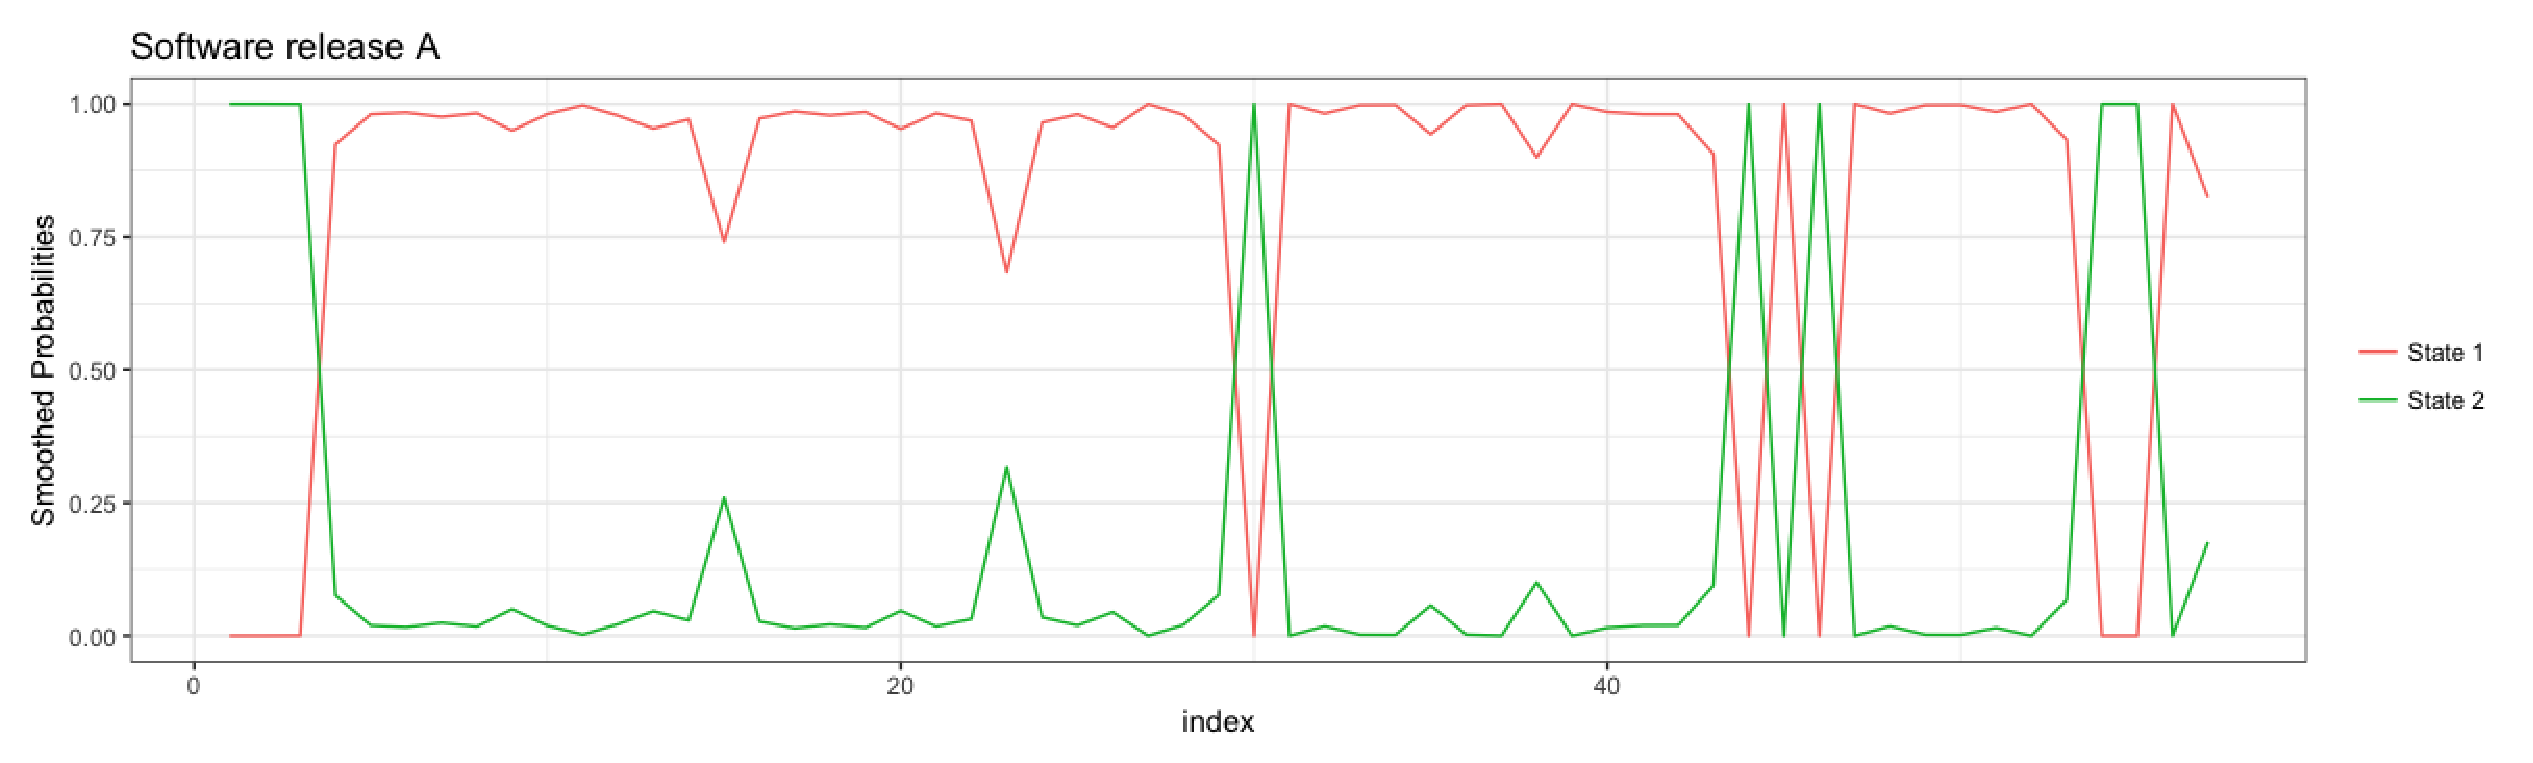
\includegraphics[scale=0.35]{picture/L16A_2_smo1}\caption{The smoothed probabilities of the software release A with two-state
model}
\label{L16A_2_smo}
\end{figure}

\begin{figure}[H]
\centering{}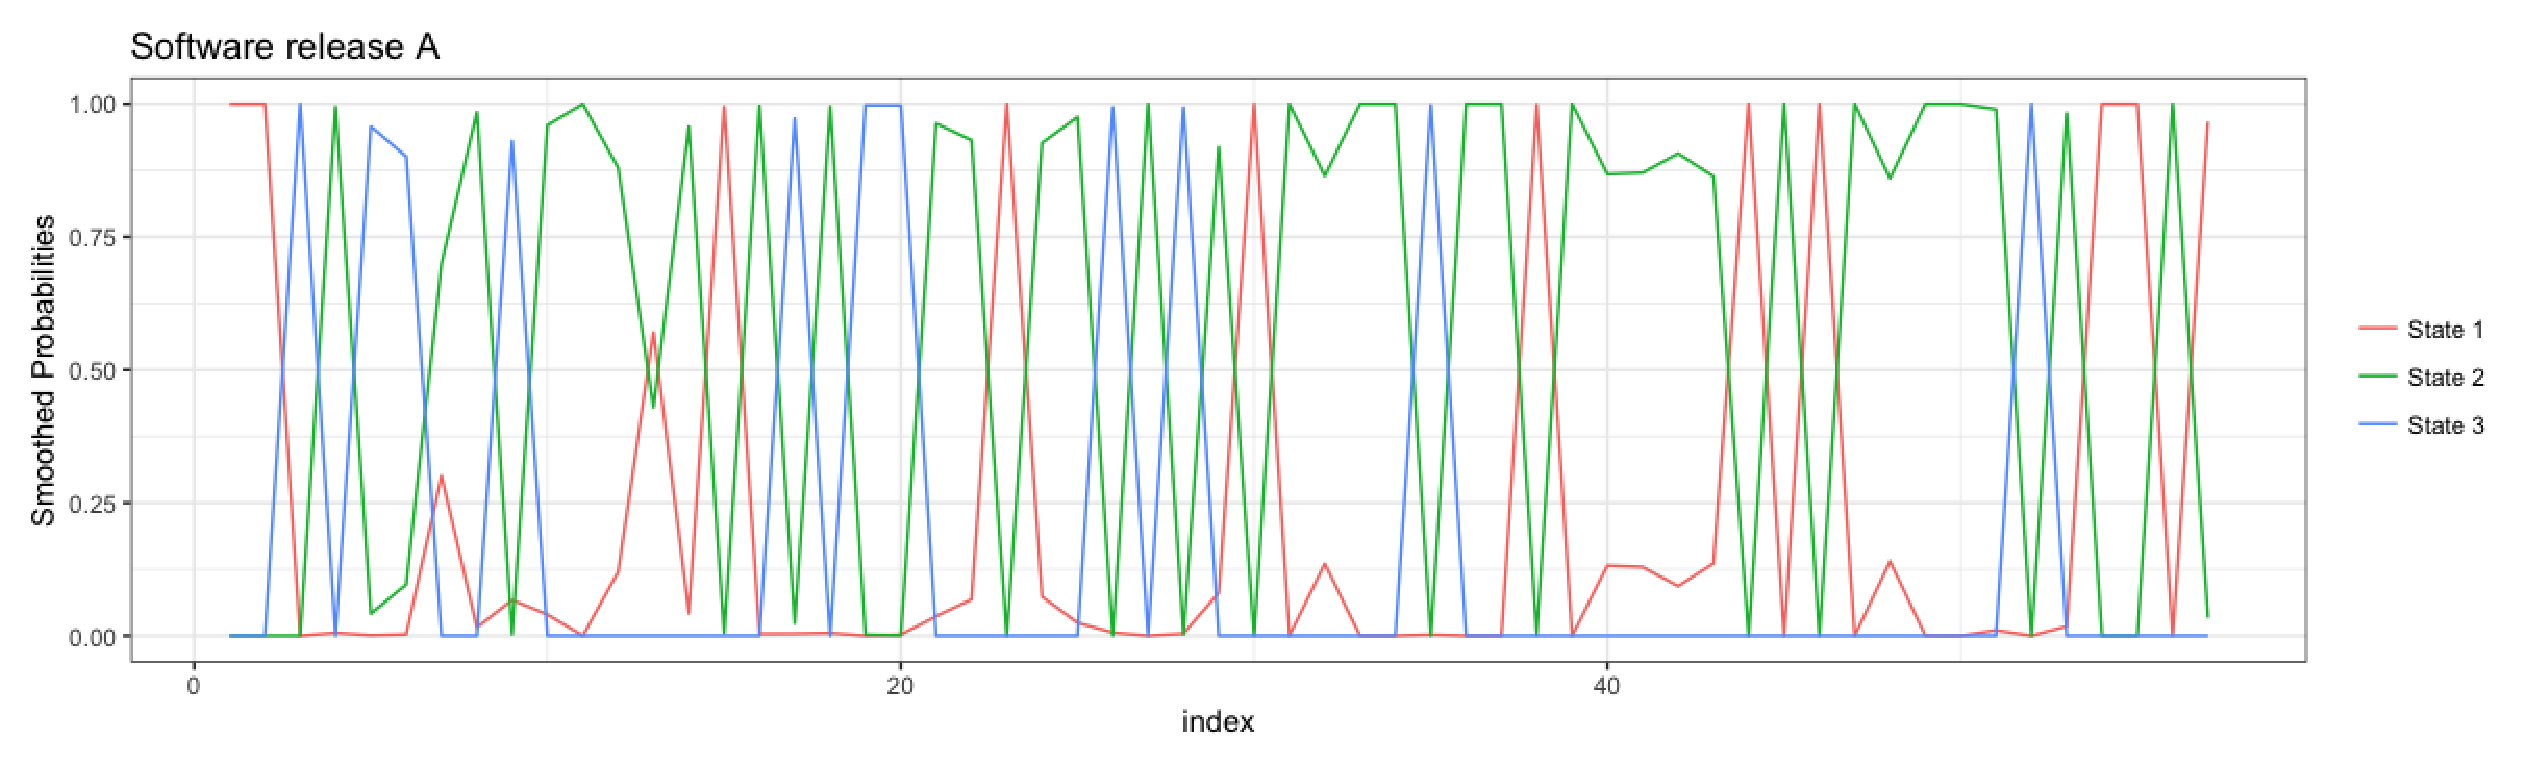
\includegraphics[scale=0.35]{picture/L16A_3_smo1}\caption{The smoothed probabilities of the software release A with three-state
model}
\label{L16A_3_smo}
\end{figure}


\subsection{Software release B}

In \ref{L16B_2_smo}, the Markov chain has several periods where it
switches back and forth between two states of the software release
B. The duration of the chain being in State2 is longer than the duration
of the chain staying in State 1. Although the chain briefly stays
in State1, it remains in this state for a few moments in the middle
of the time period (observation 91-99 and 101-114) before returning
to State2. Apparently, there are more switches between states in the
three-state model, especially in the beginning, middle, and at the
end of the period. \ref{L16B_3_smo} shows that the chain remains
in State3 over a considerable period as shown throughout observations
15-39, 42-67, and 140-170.

\begin{figure}[H]
\begin{centering}
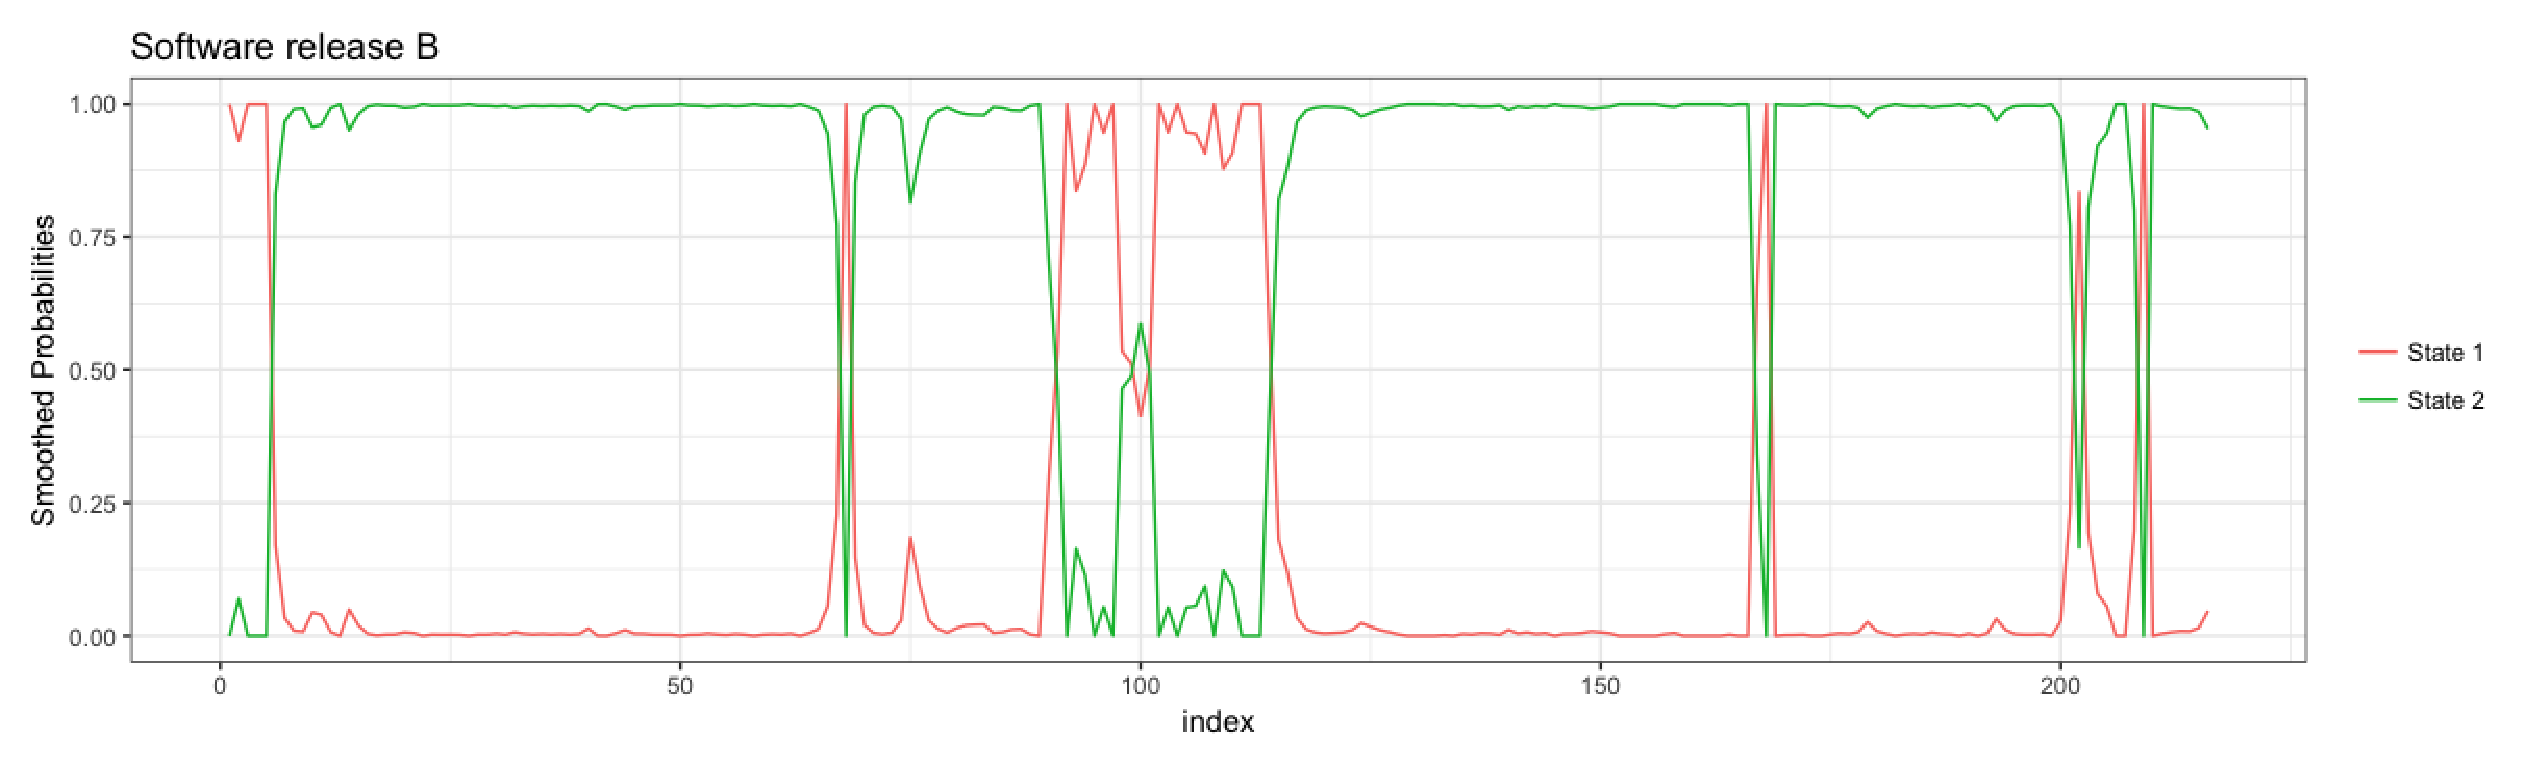
\includegraphics[scale=0.35]{picture/L16B_2_smo1}
\par\end{centering}
\caption{The smoothed probabilities of the software release B with two-state
model}
\label{L16B_2_smo}
\end{figure}

\begin{figure}[H]
\begin{centering}
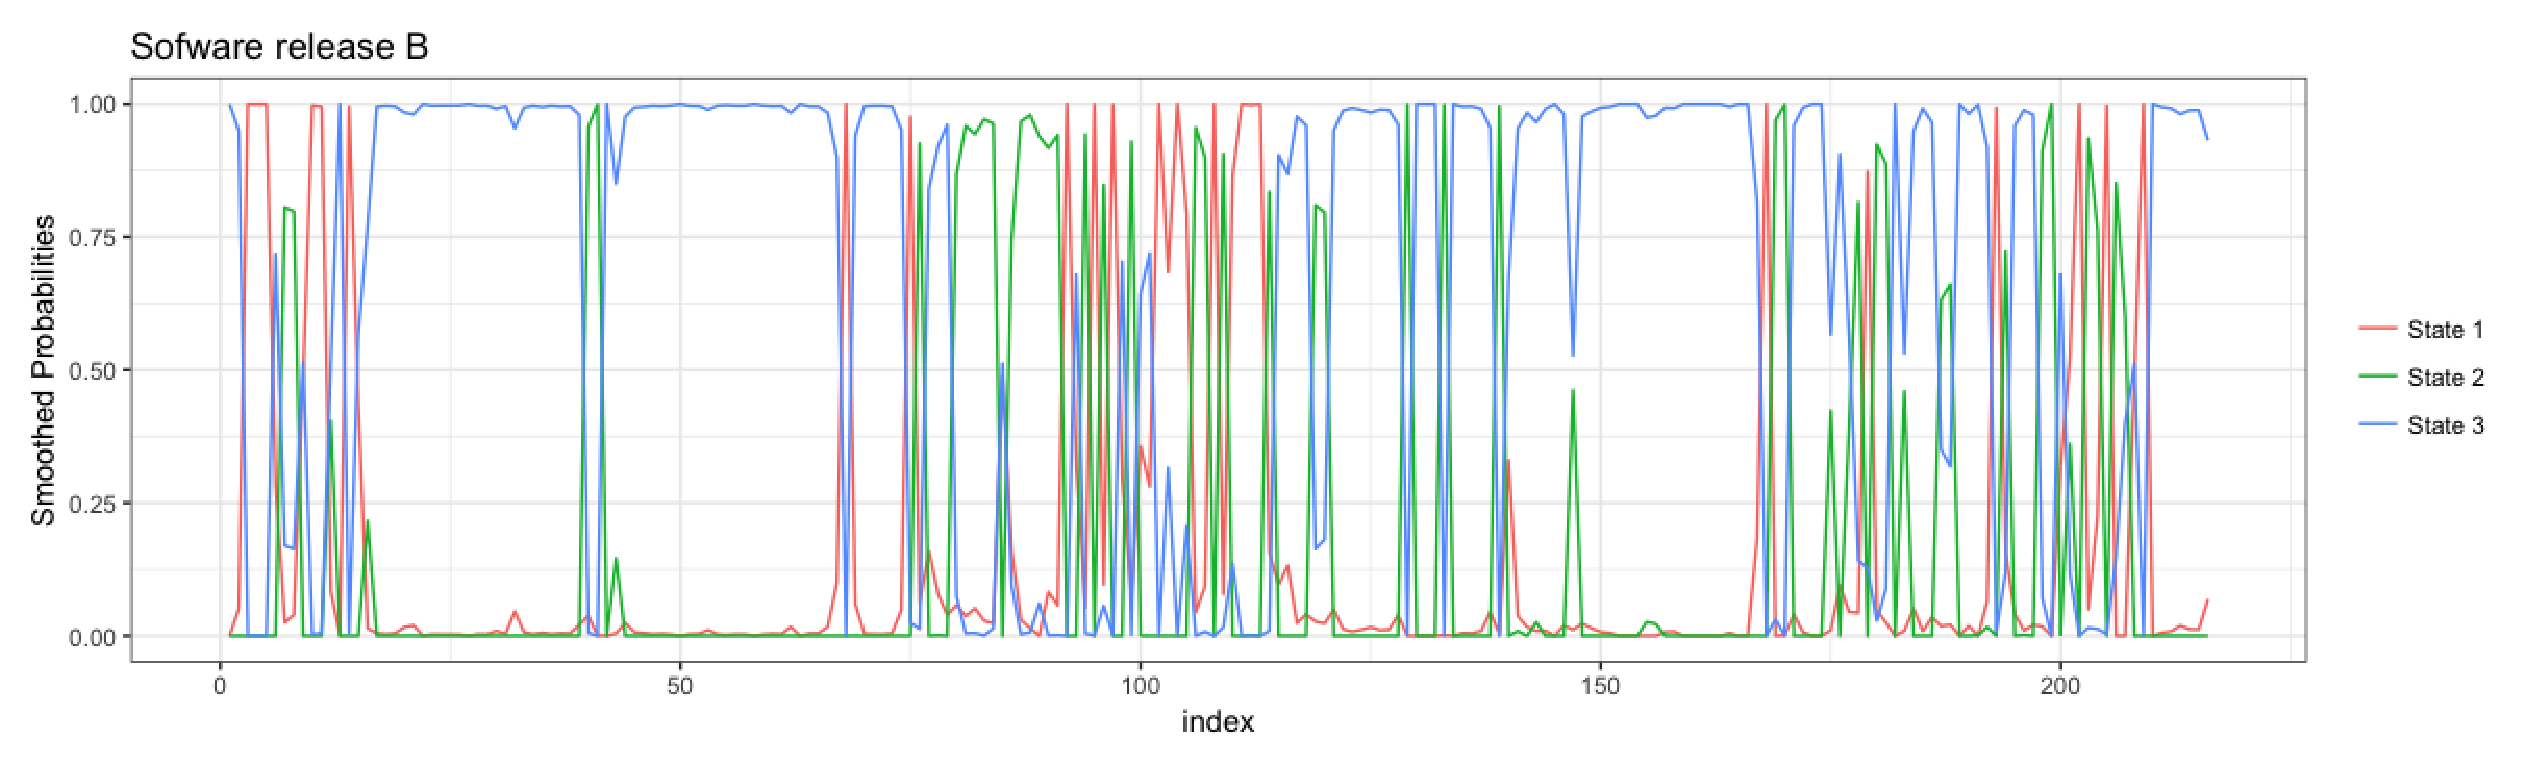
\includegraphics[scale=0.35]{picture/L16B_3_smo1}
\par\end{centering}
\caption{The smoothed probabilities of the software release B with three-state
model}
\label{L16B_3_smo}
\end{figure}

\begin{figure}[H]
\subfloat[Close-up on the observations 0-20]{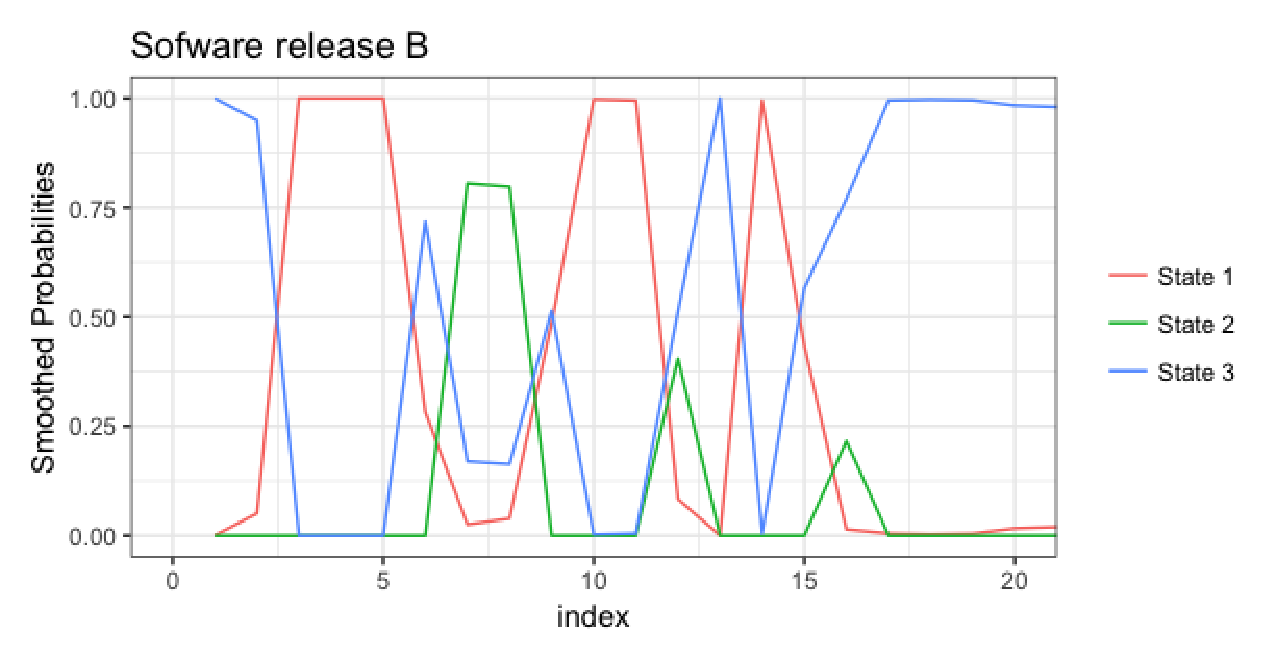
\includegraphics[scale=0.35]{picture/L16B_3_1}

}\subfloat[Close-up on the observations 75-115]{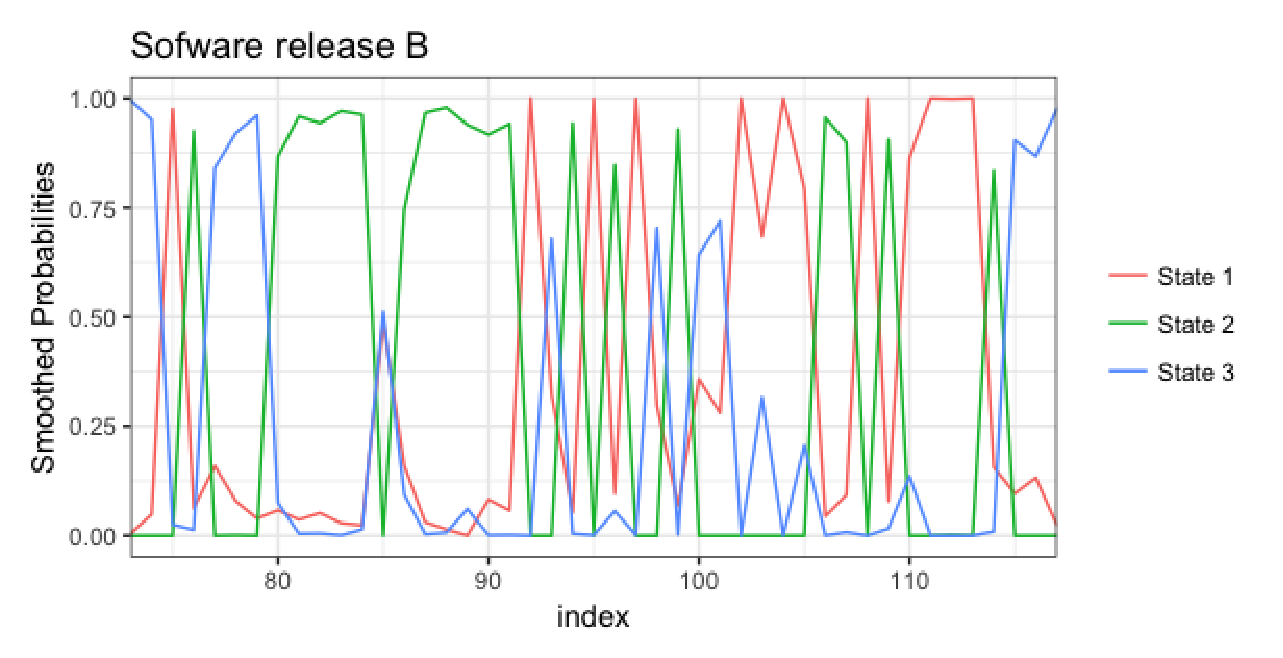
\includegraphics[scale=0.35]{picture/L16B_3_2}

}

\subfloat[Close-up on the observations 165-210]{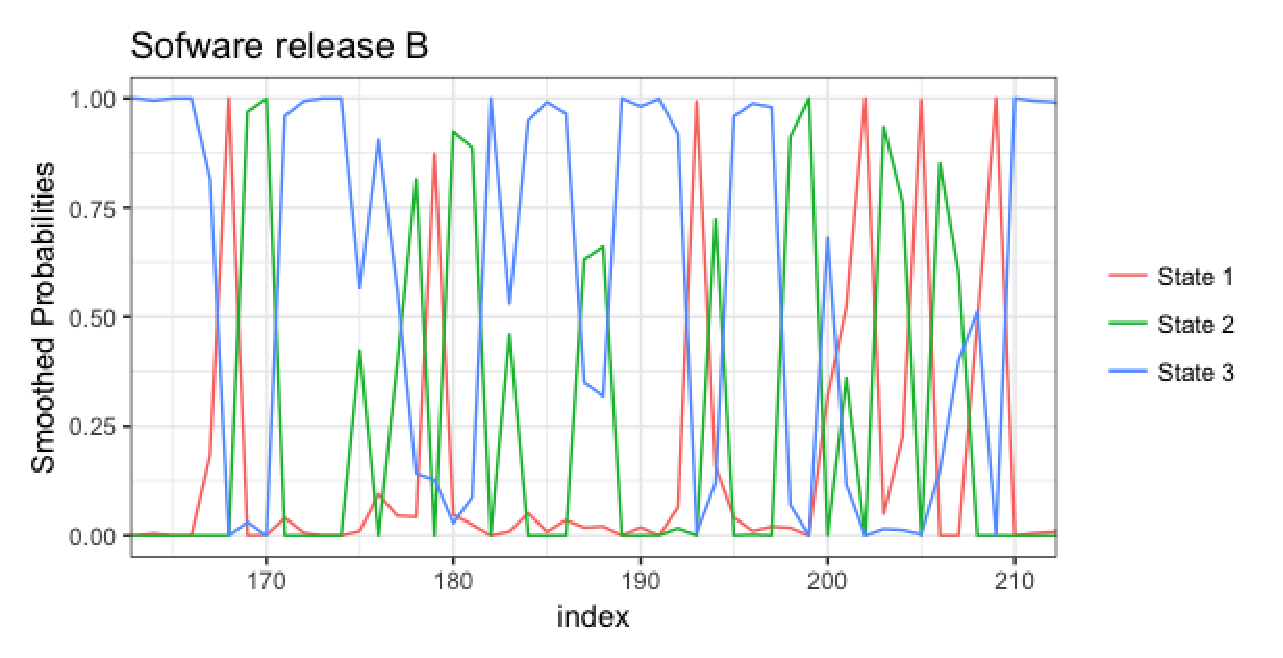
\includegraphics[scale=0.35]{picture/L16B_3_3}

}

\caption{Close-up for the smoothed probabilities of the software release B
from \ref{L16B_3_smo}}
\end{figure}


\subsection{Software release C}

There are a number of switches between states in the two-state model
of the software release C. In \ref{L17A_2_smo}, when the Markov chain
is in State1, it continues to stay in its state for a while before
leaving to State2. Furthermore, the chain stays a fairly short duration
in State2. After the chain visits State2, it instantly switches back
to State1. \ref{L17A_3_smo} presents the chain which has many switches
between State1 and State3 in the first half of the time period. The
chain for the three-state model also stays in State2 significantly
long from observation 104 to 129, which is the end of the time series.

\begin{figure}[H]
\centering{}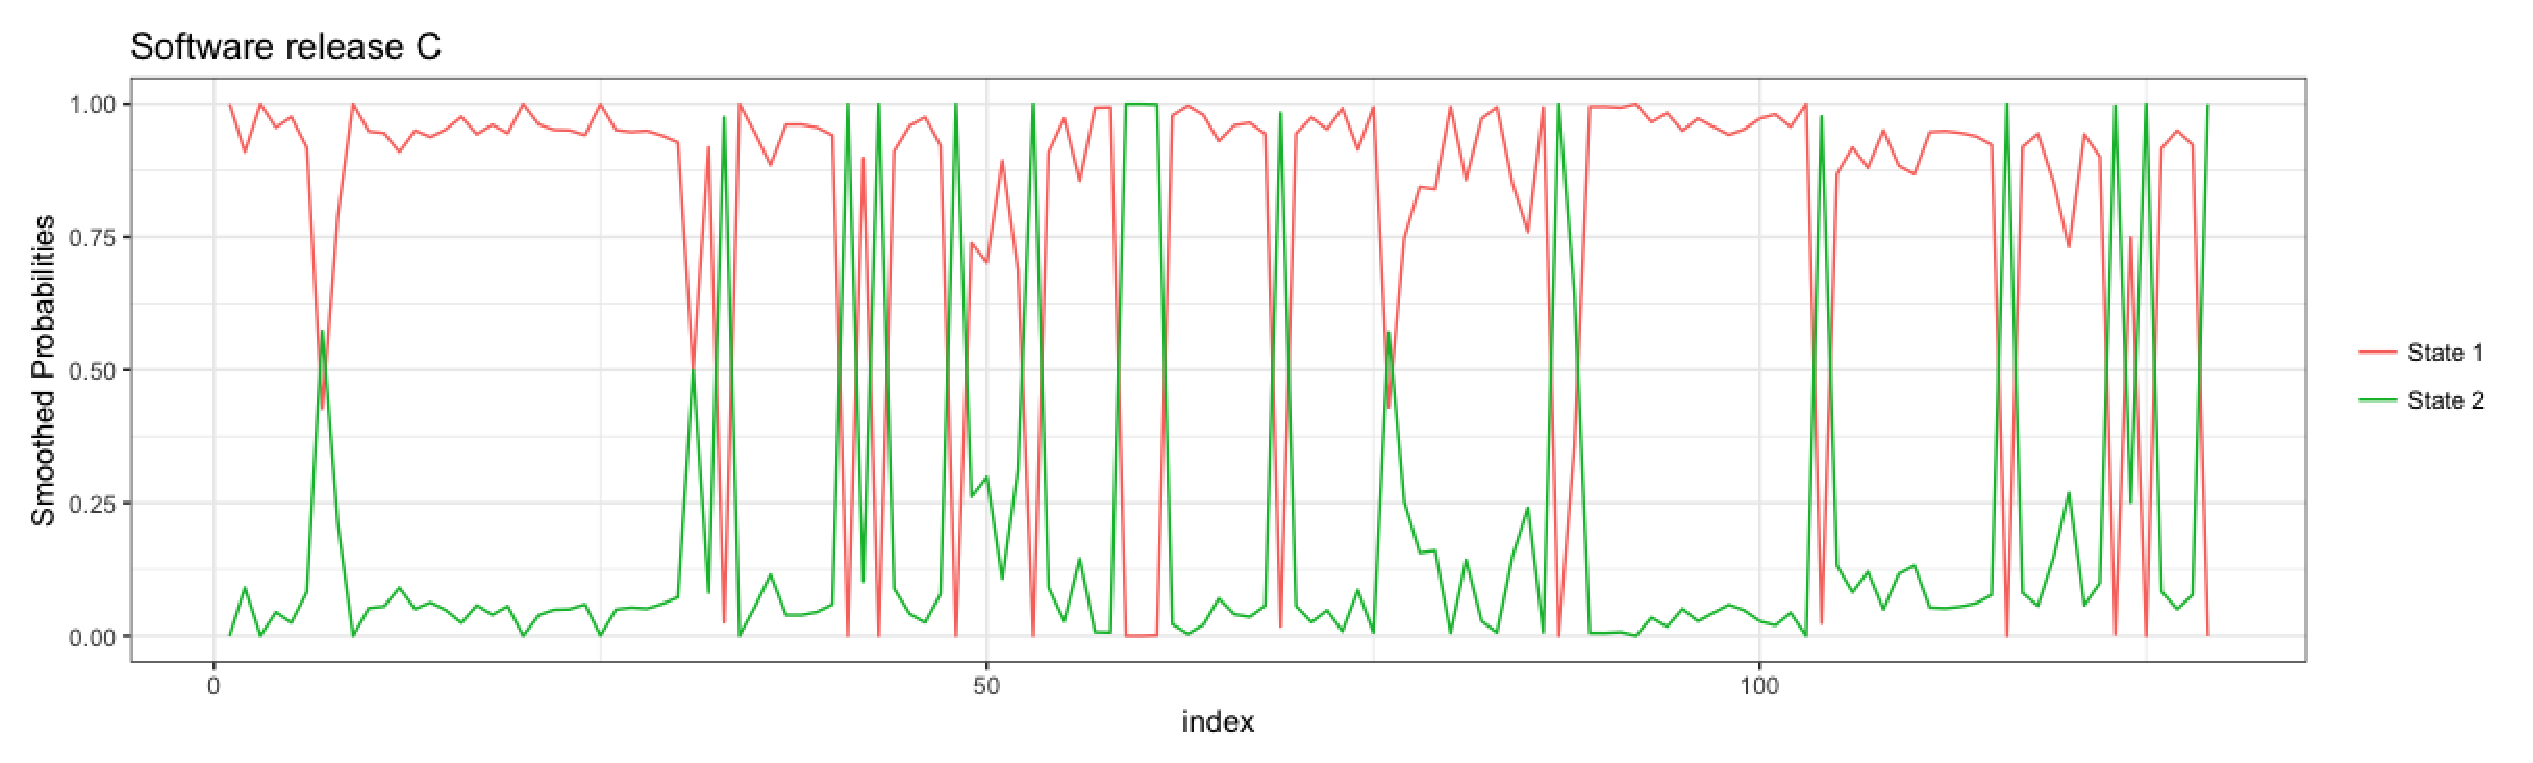
\includegraphics[scale=0.35]{picture/L17A_2_smo1}\caption{The smoothed probabilities of the software release C with two-state
model}
\label{L17A_2_smo}
\end{figure}
\begin{figure}[H]
\centering{}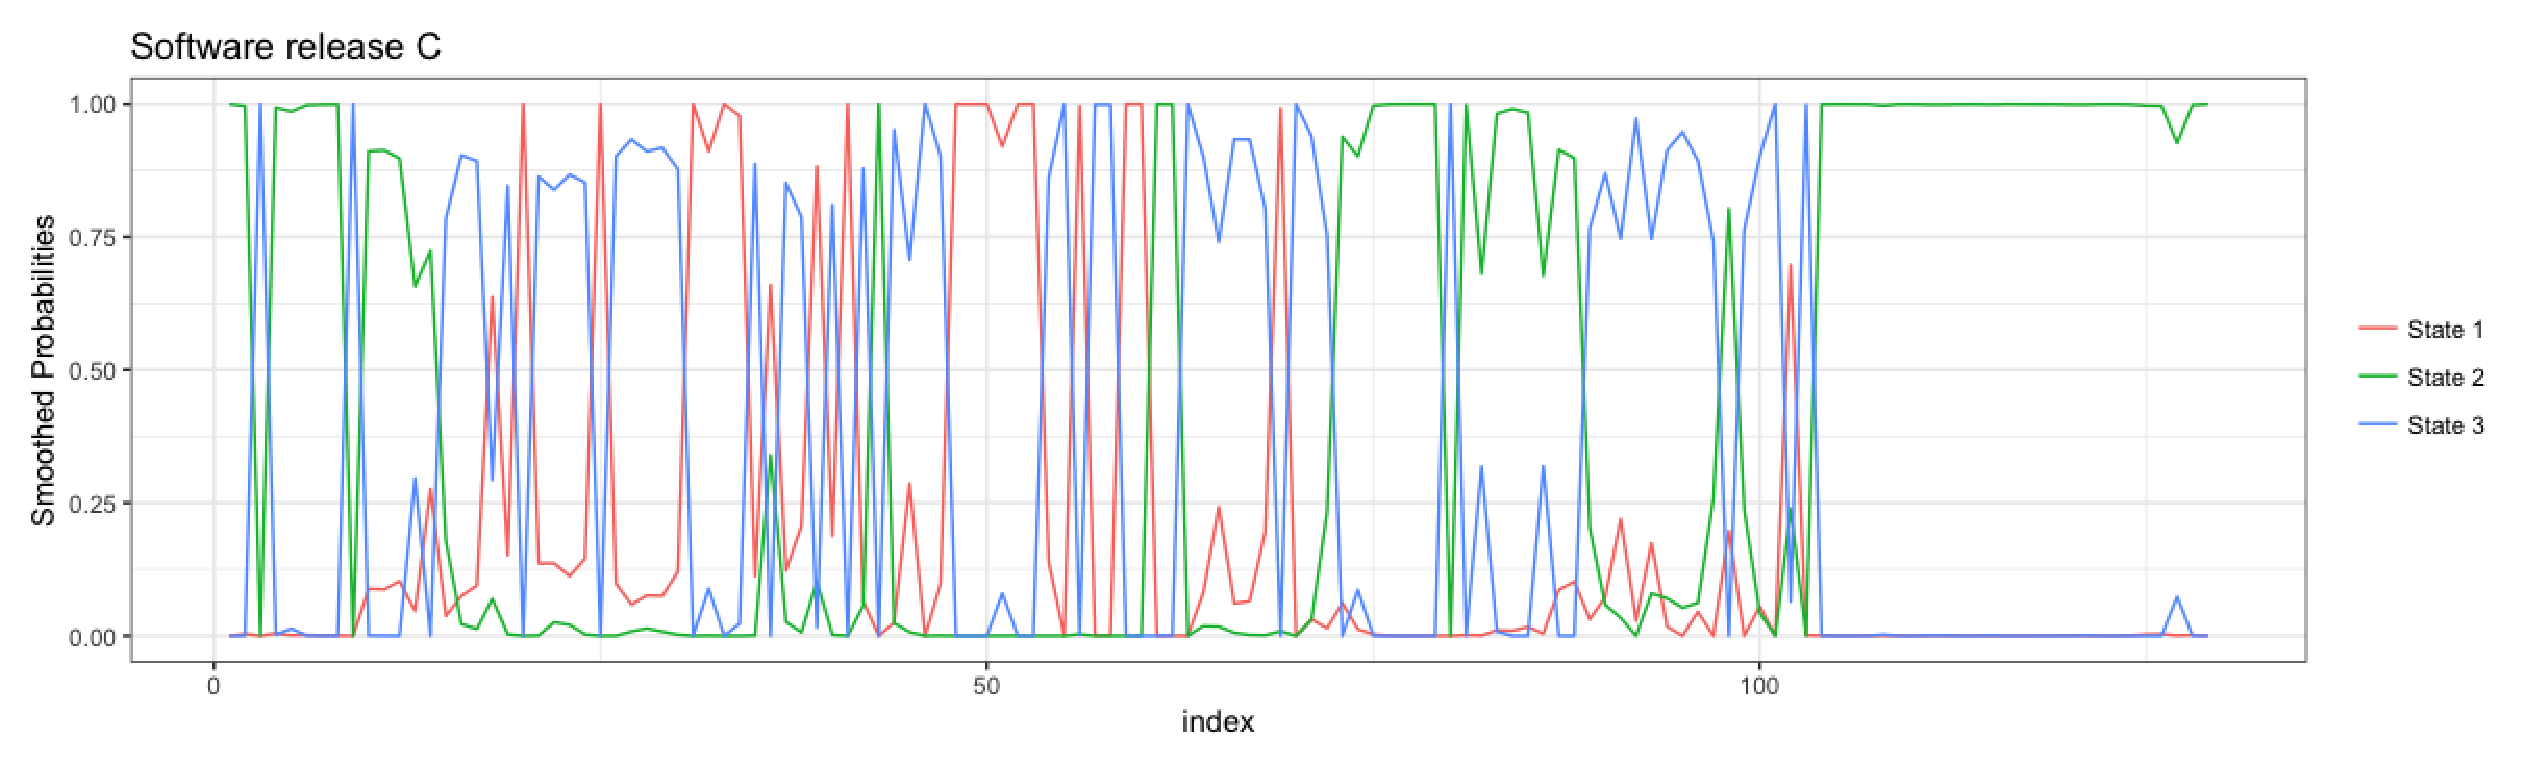
\includegraphics[scale=0.35]{picture/L17A_3_smo1}\caption{The smoothed probabilities of the software release C with three-state
model}
\label{L17A_3_smo}
\end{figure}

\begin{figure}[H]
\subfloat[Close-up on the observations 15-45]{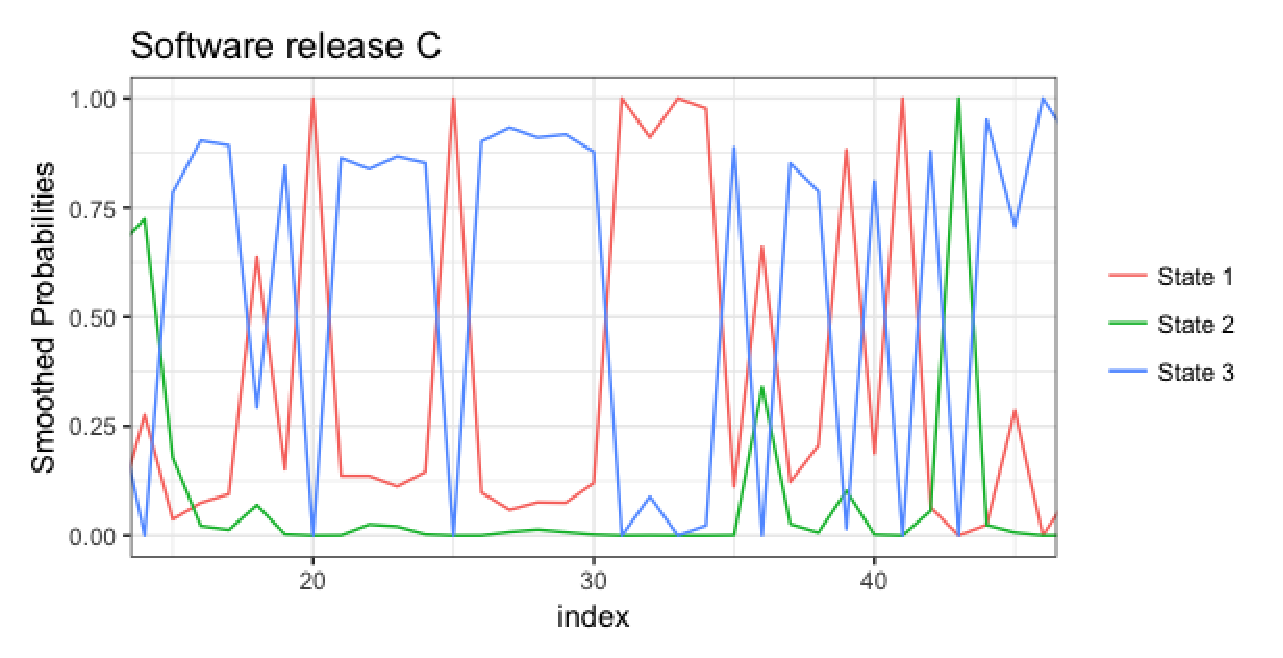
\includegraphics[scale=0.35]{picture/L17A_3_1}

}

\caption{Close-up for the smoothed probabilities of the software release C
from \ref{L17A_3_smo}}

\end{figure}

After examining the outputs from the models along with the plots,
the three-state models for each software release were further analyzed
in the thesis. More details are provided in \ref{chap:Discussion}. 

\section{Analysis II: Number of Switching coefficients \label{sec:Switching}}

In this section, the number of switching coefficients to be included
in the model were decided based on applying the Markov switching model
with the selected number of states from Analysis I i.e., three-state
Markov switching model. The fitted Markov switching models in Analysis
I were performed by assuming that every parameter in the model had
switching effects i.e., coefficients can have different values in
different periods. However, in practice, each coefficient can have
either a switching or non-switching effect. Therefore, Markov switching
models were applied to each dataset again but with a hypothesis that
the variables considered as a test environment are possible to have
non-switching effects. In this section, the structure of all the models
from all three datasets are reported in the tables. The best model
is selected for each dataset and its state specification is presented
in the plots. Further discussion and details about these chosen models
are provided in \ref{subsec:Model-selection}. It should be noted
that these three chosen models will later be used throughout this
thesis, and the model outputs are shown in \ref{chap:Output}. 

\subsection{Software release A}

For the dataset of the software release A, \emph{DuProdName} was not
included in the model fitting as explained previously. Only two variables
of the test environment were left to try whether they could have non-switching
effects or not. The result is shown in \ref{L16A_switch}. The second
model has the highest BIC and even higher than the model which have
all switching coefficients. The first model, where both \emph{Fdd/Tdd}
and \emph{NumCells} do not have switching effects, was selected to
be used with this dataset. 

\begin{table}[h]
\caption{List of the model structure of the software release A along with its
BIC. The last line is the result taken from the three-state model
in the Analysis I. The line in bold indicates the selected model.}
\label{L16A_switch}
\centering{}%
\begin{tabular}{cccc}
\toprule 
\multirow{2}{*}{Model} & \multicolumn{2}{c}{Switching effect} & \multirow{2}{*}{BIC}\tabularnewline
\cmidrule{2-3} 
 & Fdd/Tdd & NumCells & \tabularnewline
\midrule
\midrule 
\textbf{1} & \textbf{N} & \textbf{N} & \textbf{413.408}\tabularnewline
2 & N & Y & 438.371\tabularnewline
3 & Y & N & 401.232\tabularnewline
\midrule
 & Y & Y & 417.682\tabularnewline
\bottomrule
\end{tabular}
\end{table}

\ref{L16A_NN} indicates the CPU utilization of the software release
A and also shows the periods of the derived state from the model.
From the plot, State2 clearly has the longest duration without switching
state. When the chain moves to either State1 or State3, most of the
time it immediately switches to another state. However, the duration
when the chain stays in State1 is longer in the beginning and almost
at the end of the period. Another characteristic that could be observed
is that State2 switches more often to State3 rather than to State1.
In the plot, there is a period where there is no significant change
in the CPU utilization (observations 15-25) but there are some switches
between states. Besides, there are some abrupt changes which are not
detected by the model such as observation 11. 

\begin{figure}[H]
\centering{}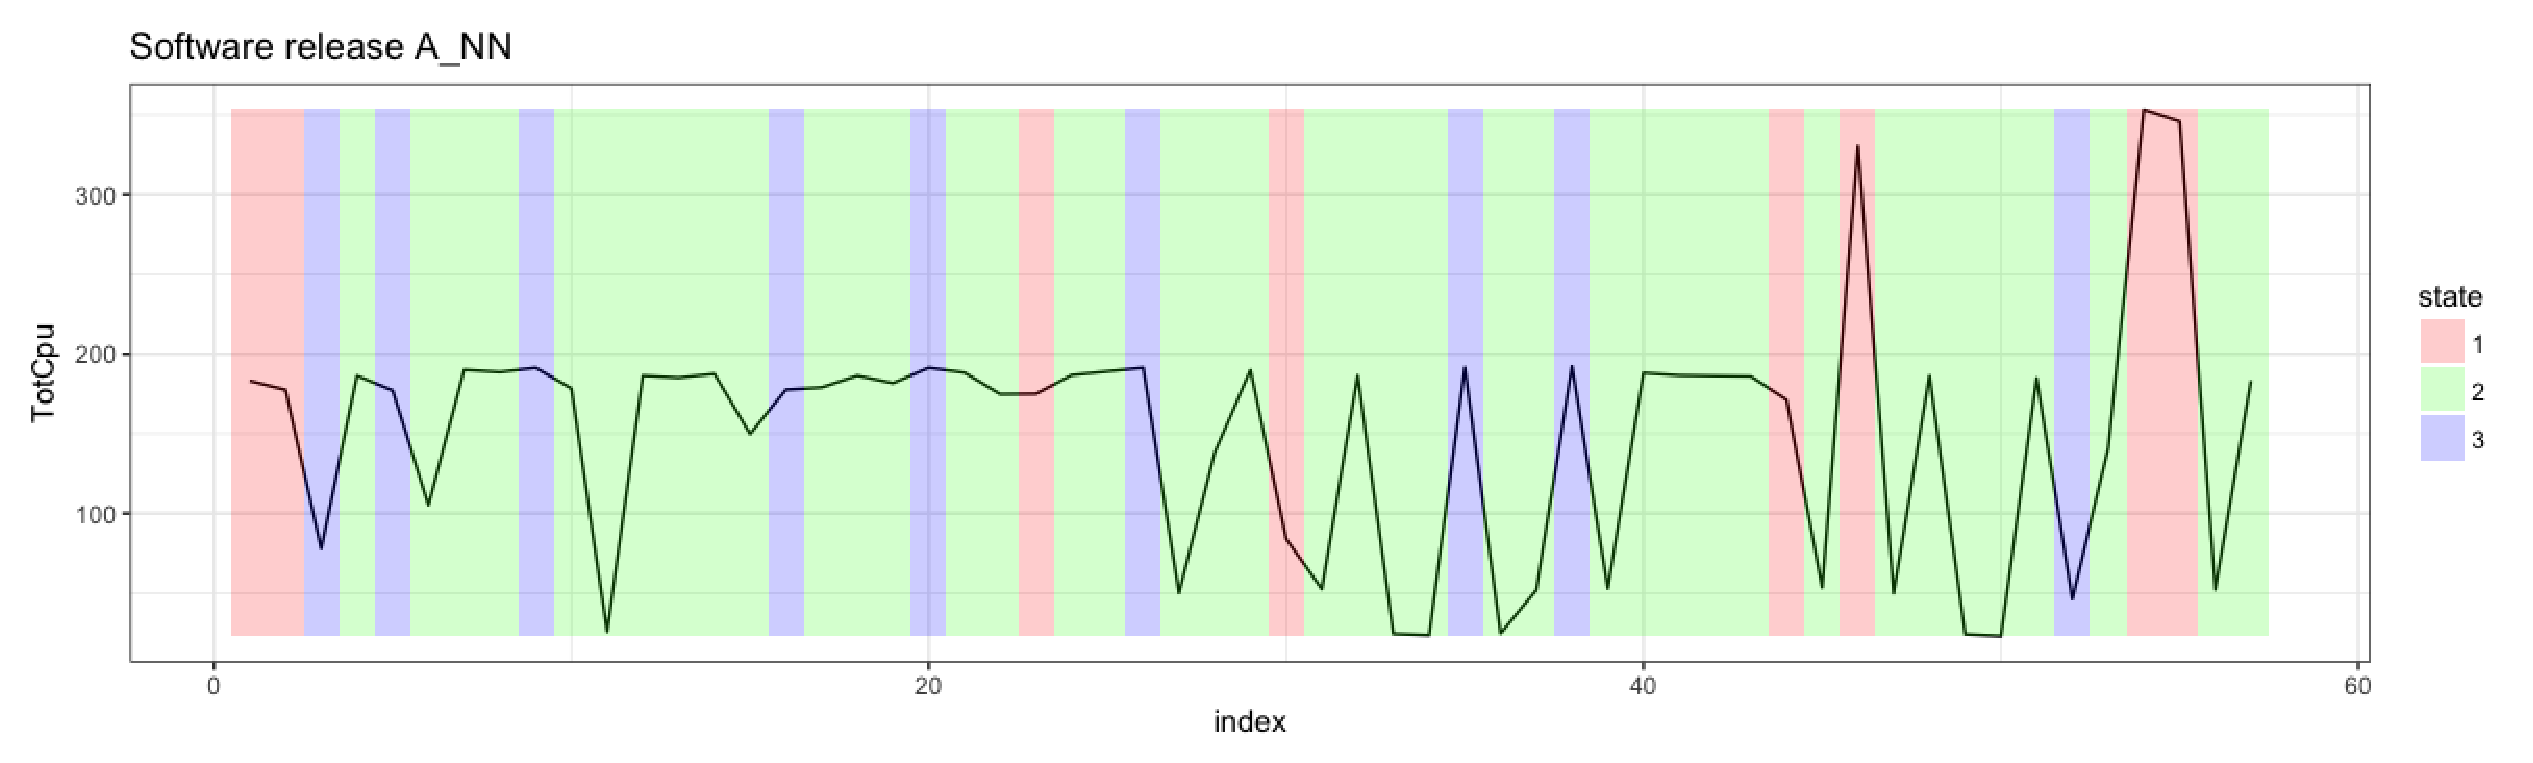
\includegraphics[scale=0.35]{picture/L16A_NN1}\caption{The CPU utilization of the software release A showing the periods
where the observation is in the specific state. \protect \\
Model 1: Fdd/Tdd and Numcells are non-switching coefficients.}
\label{L16A_NN}
\end{figure}


\subsection{Software release B}

For the software release B, \ref{L16B_switch} presents the results
of fitting the model with different combinations of switching coefficients.
Models 5 and 7 have higher BICs than the model which have switching
effects in all coefficients. The second model, where \emph{DuProdName}
and \emph{Fdd/Tdd} are non-switching coefficients, has the smallest
BIC. The chosen model for this dataset is the model which has only
\emph{DuProdName} as a non-switching coefficient or model 4.

\begin{table}[h]
\caption{List of the model structure of the software release B along with its
BIC. The last line is the result taken from the three-state model
in the Analysis I. The line in bold indicates the selected model.}
\label{L16B_switch}
\centering{}%
\begin{tabular}{ccccc}
\toprule 
\multirow{2}{*}{Model} & \multicolumn{3}{c}{Switching effect} & \multirow{2}{*}{BIC}\tabularnewline
\cmidrule{2-4} 
 & DuProdName & Fdd/Tdd & NumCells & \tabularnewline
\midrule
\midrule 
1 & N & N & N & 1787.528\tabularnewline
2 & N & N & Y & 1704.393\tabularnewline
3 & N & Y & N & 1784.384\tabularnewline
\textbf{4} & \textbf{N} & \textbf{Y} & \textbf{Y} & \textbf{1776.102}\tabularnewline
5 & Y & N & N & 1806.385\tabularnewline
6 & Y & N & Y & 1725.865\tabularnewline
7 & Y & Y & N & 1804.487\tabularnewline
\midrule
 & Y & Y & Y & 1797.259\tabularnewline
\bottomrule
\end{tabular}
\end{table}

Many switches between states can easily be seen in \ref{L16B_NYY}.
However, the state which has the longest duration remaining in its
own state is State3. There are three durations where the chain stays
in State3 for a long period of time. Another noticeable behavior from
this switching mechanism is that there are several switches to State1
and State2 in the beginning, middle, and at the end of the time period.
There are periods where the CPU utilization value does not change
much but the model identifies some switches. Also, there are periods
where the model fails to detect changes which is rather obvious.

\begin{figure}[H]
\begin{centering}
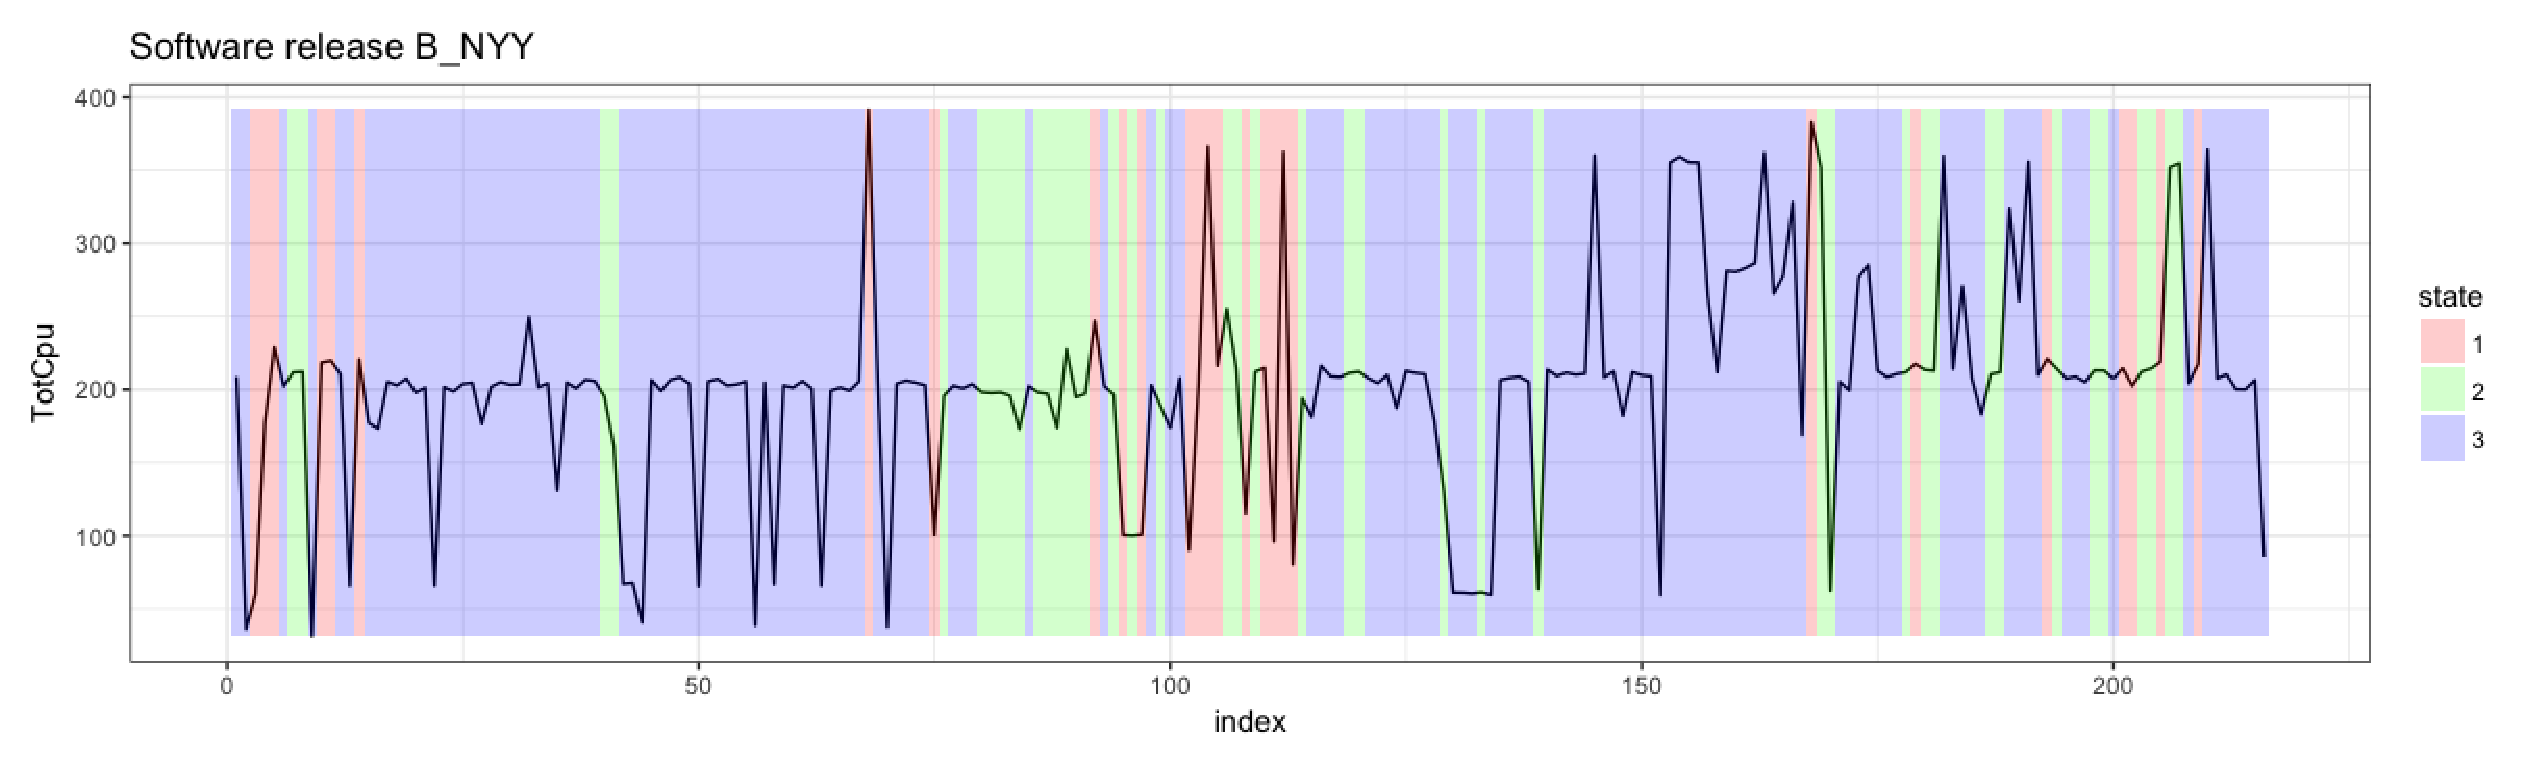
\includegraphics[scale=0.35]{picture/L16B_NYY1}
\par\end{centering}
\caption{The CPU utilization of the software release B showing the periods
where the observation is in the specific state. \protect \\
Model 4: DuProdName is non-switching coefficient.}
\label{L16B_NYY}
\end{figure}


\subsection{Software release C}

\ref{L17A_switch} presents model structure of the software release
C. Only model 2 has higher BIC than the model which have all switching
coefficients. The least BIC is from the first model of which all three
variables in the test environment have non-switching effects. This
model was also chosen to be further used for this dataset.

\begin{table}[h]
\caption{List of the model structure of the software release C along with its
BIC. The last line is the result taken from the three-state model
in the Analysis I. The line in bold indicates the selected model.}
\label{L17A_switch}
\centering{}%
\begin{tabular}{ccccc}
\toprule 
\multirow{2}{*}{Model} & \multicolumn{3}{c}{Switching effect} & \multirow{2}{*}{BIC}\tabularnewline
\cmidrule{2-4} 
 & DuProdName & Fdd/Tdd & NumCells & \tabularnewline
\midrule
\midrule 
\textbf{1} & \textbf{N} & \textbf{N} & \textbf{N} & \textbf{1140.474}\tabularnewline
2 & N & N & Y & 1204.280\tabularnewline
3 & N & Y & N & 1152.740\tabularnewline
4 & N & Y & Y & 1184.643\tabularnewline
5 & Y & N & N & 1146.000\tabularnewline
6 & Y & N & Y & 1189.236\tabularnewline
7 & Y & Y & N & 1157.311\tabularnewline
\midrule
 & Y & Y & Y & 1199.075\tabularnewline
\bottomrule
\end{tabular}
\end{table}

Several switches between three states occur in the beginning of the
time series as shown in \ref{L17A_NNN}. Around the end of the time
series period, State3 appears to have a longer duration and fewer
switches to State1. State2 seems to be the only state which has a
fairly short duration for the chain to stay in the state. Furthermore,
State2 tends to switch to State1 more often than to switch to State3.
The plot indicates some missed detections for this model which is
happened mostly in the durations of State3. 

\begin{figure}[H]
\begin{centering}
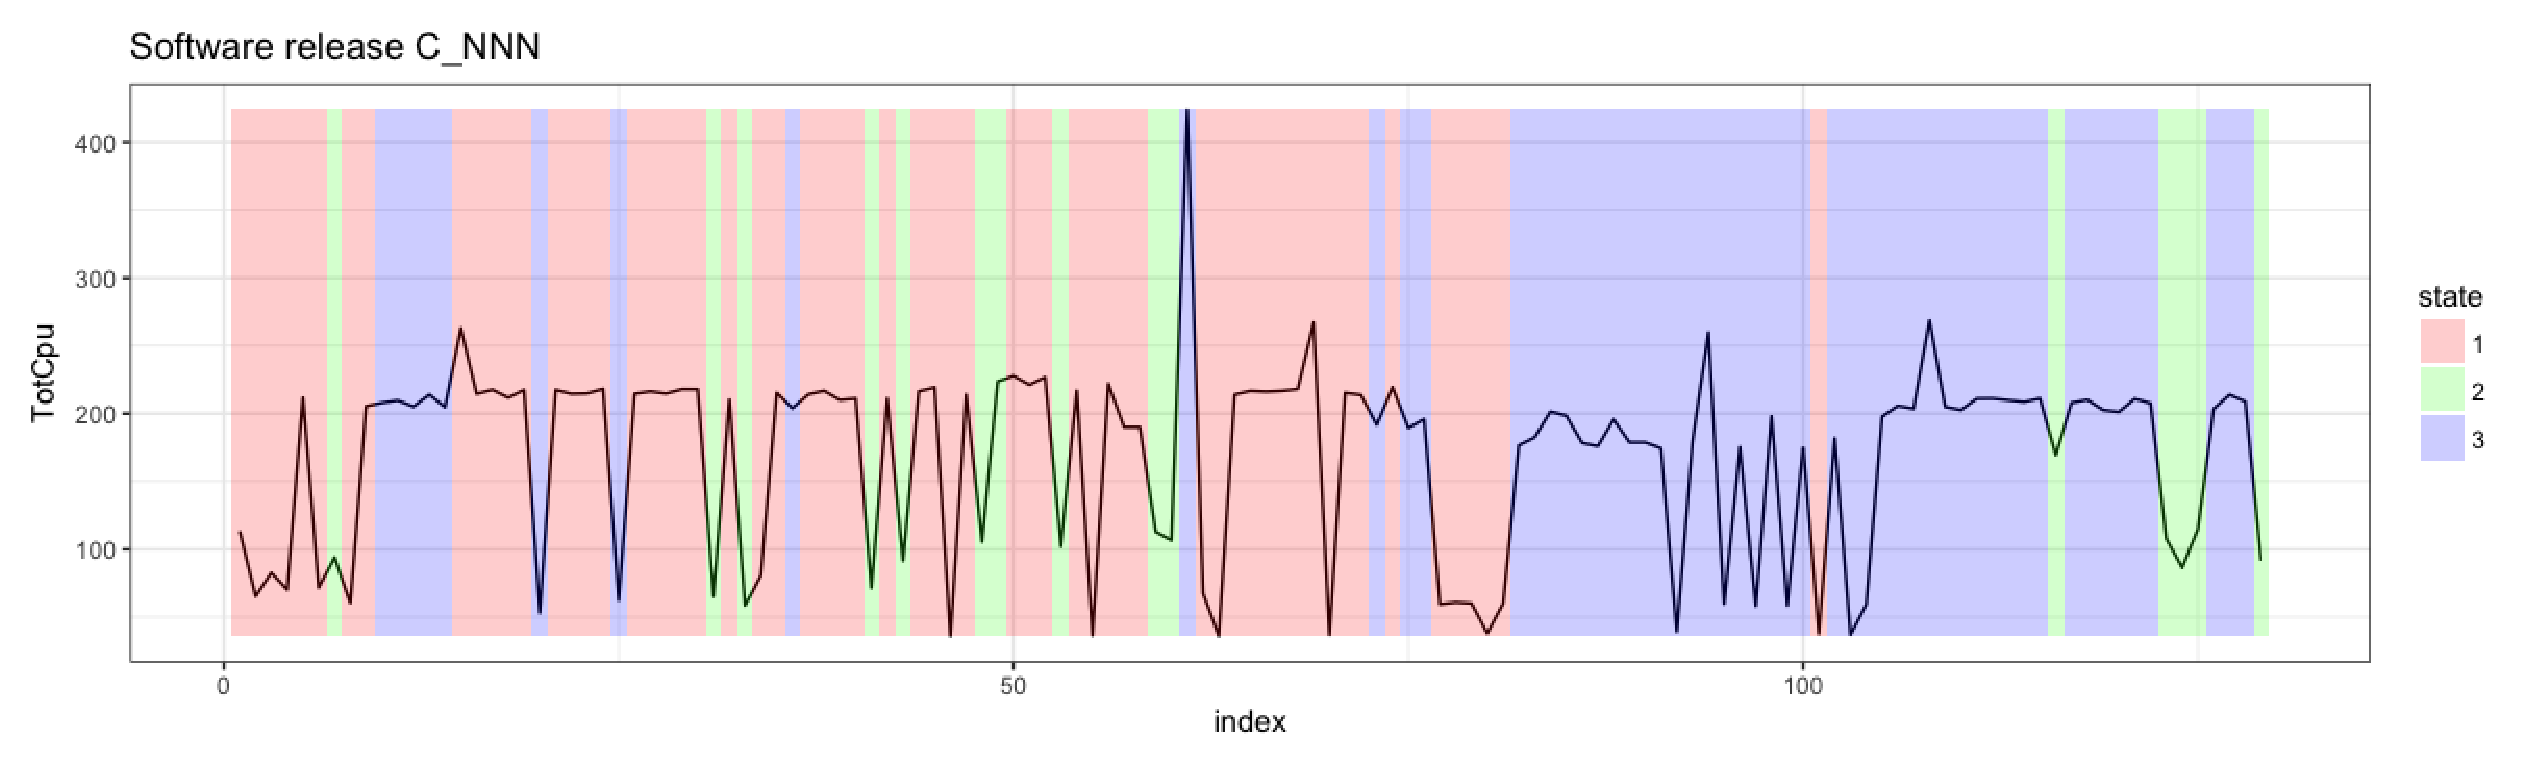
\includegraphics[scale=0.35]{picture/L17A_NNN1}
\par\end{centering}
\caption{The CPU utilization of the software release C showing the periods
where the observation is in the specific state. \protect \\
Model 1: DuProdName, Fdd/Tdd, and NumCells are non-switching coefficients.}
\label{L17A_NNN}
\end{figure}


\section{Residual analysis\label{sec:Residual}}

Pooled residuals of the selected Markov switching model from \ref{sec:Switching}
were analyzed to determine how well the model fitted with an assumption
of a normal distribution. A Quantile-Quantile (Q-Q) plot is an effective
tool for assessing normality. Moreover, an Autocorrelation function
(ACF) and a Partial Autocorrelation Function (PACF) of residuals are
a useful technique to check on the independence of noise terms in
the model. The Q-Q plot and the ACF/PACF plots play a significant
role in the residual diagnostics. These plots of each dataset are
shown in \ref{L16A_plotDiag}, \ref{L16B_plotDiag}, and \ref{L17A_plotDiag}. 

\subsection{Software release A}

In \ref{L16A_plotDiag}, the pooled residuals appear to fall in a
straight line with some deviations in its tails. There is an evidence
of autocorrelation in the residuals of this model, which can be seen
in both ACF and PACF plot, at lag 8. 

\begin{figure}[h]
\begin{centering}
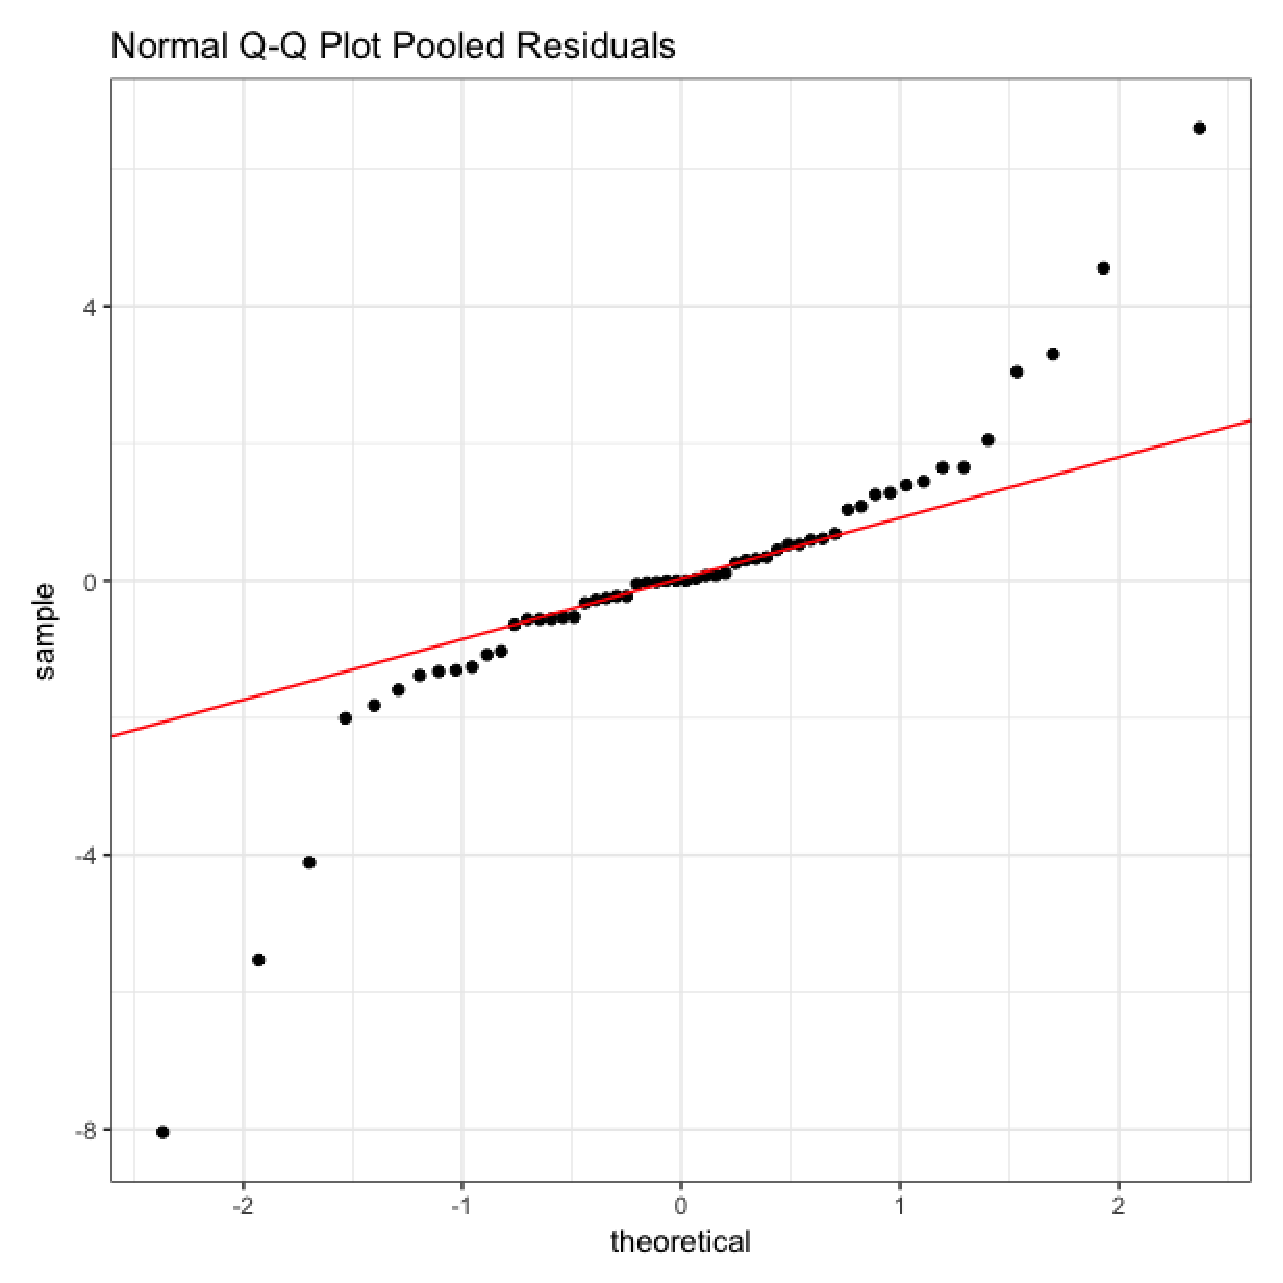
\includegraphics[scale=0.3]{picture/L16A_QQPool}$\quad$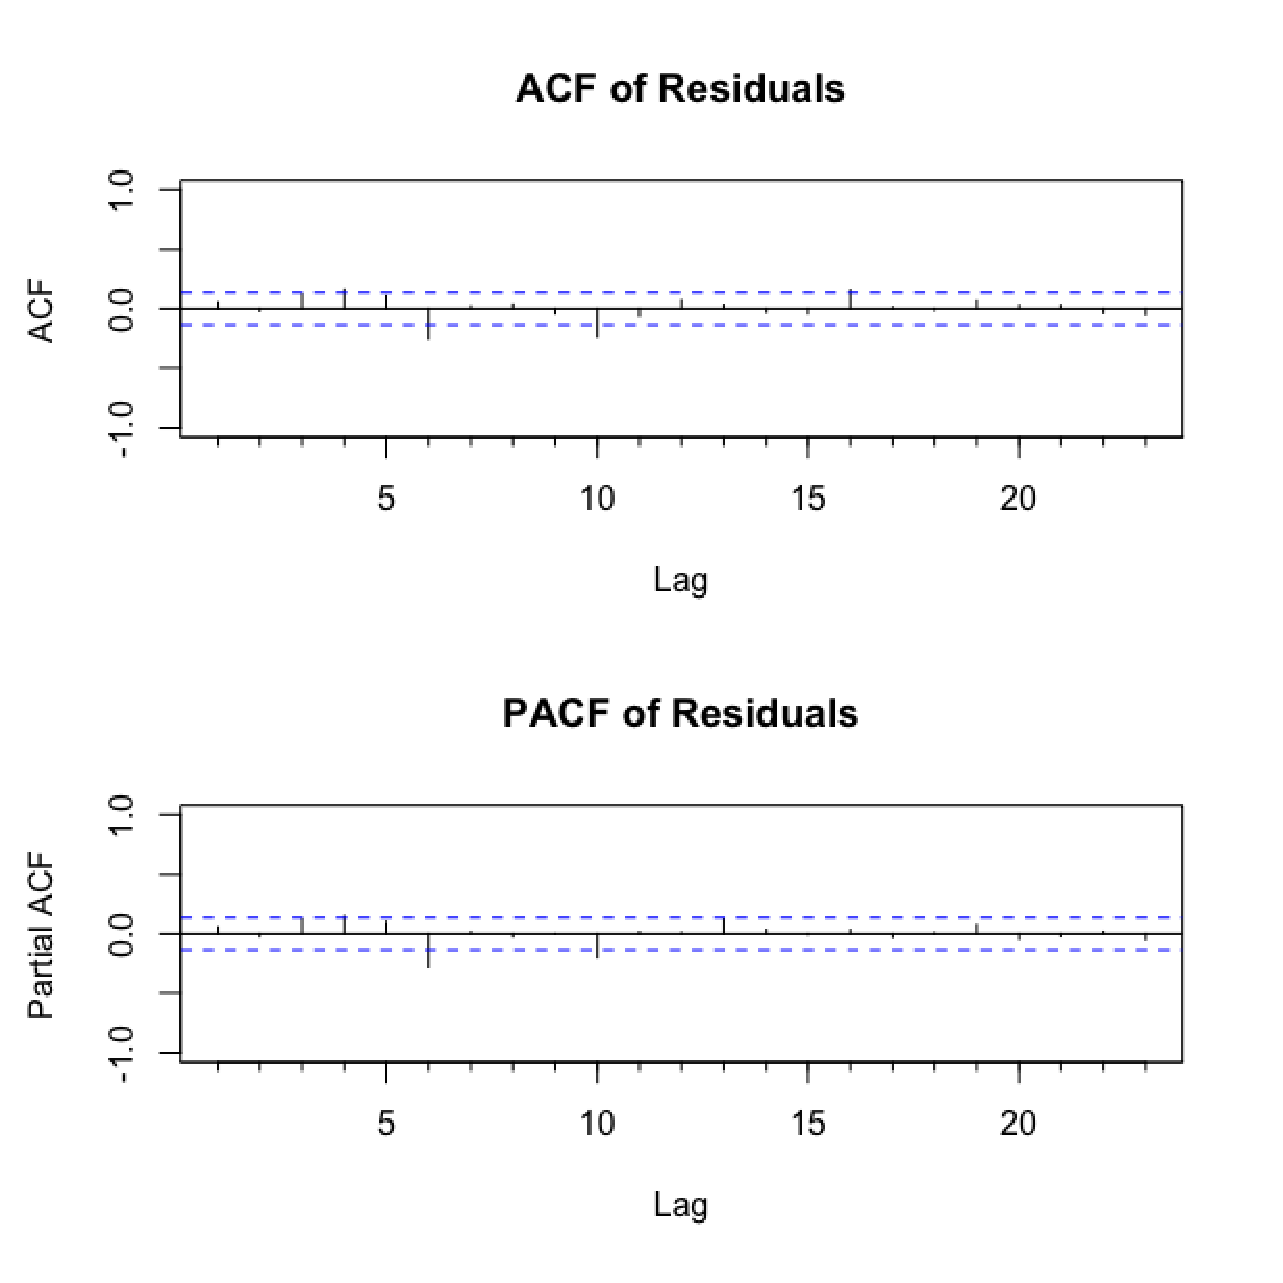
\includegraphics[scale=0.3]{picture/L16A_ACFPool}
\par\end{centering}
\caption{The normal Q-Q plot and the ACF/PACF of pooled residuals of the software
release A}
\label{L16A_plotDiag}
\end{figure}


\subsection{Software release B}

\ref{L16B_plotDiag} presents points that form a straight line in
the middle of the plot, but curve off at both ends. This is a characteristic
of a heavy-tailed distribution. The data has more extreme values than
it should if the data truly comes from a normal distribution. In addition,
both the ACF and PACF plots show that there is a small amount of autocorrelation
remaining in the residuals. The statistically significant correlation
of this model is at lags 6 and 10. The significance at lag 4 both
in the ACF and PACF plots is slightly higher than two standard errors.

\begin{figure}[H]
\begin{centering}
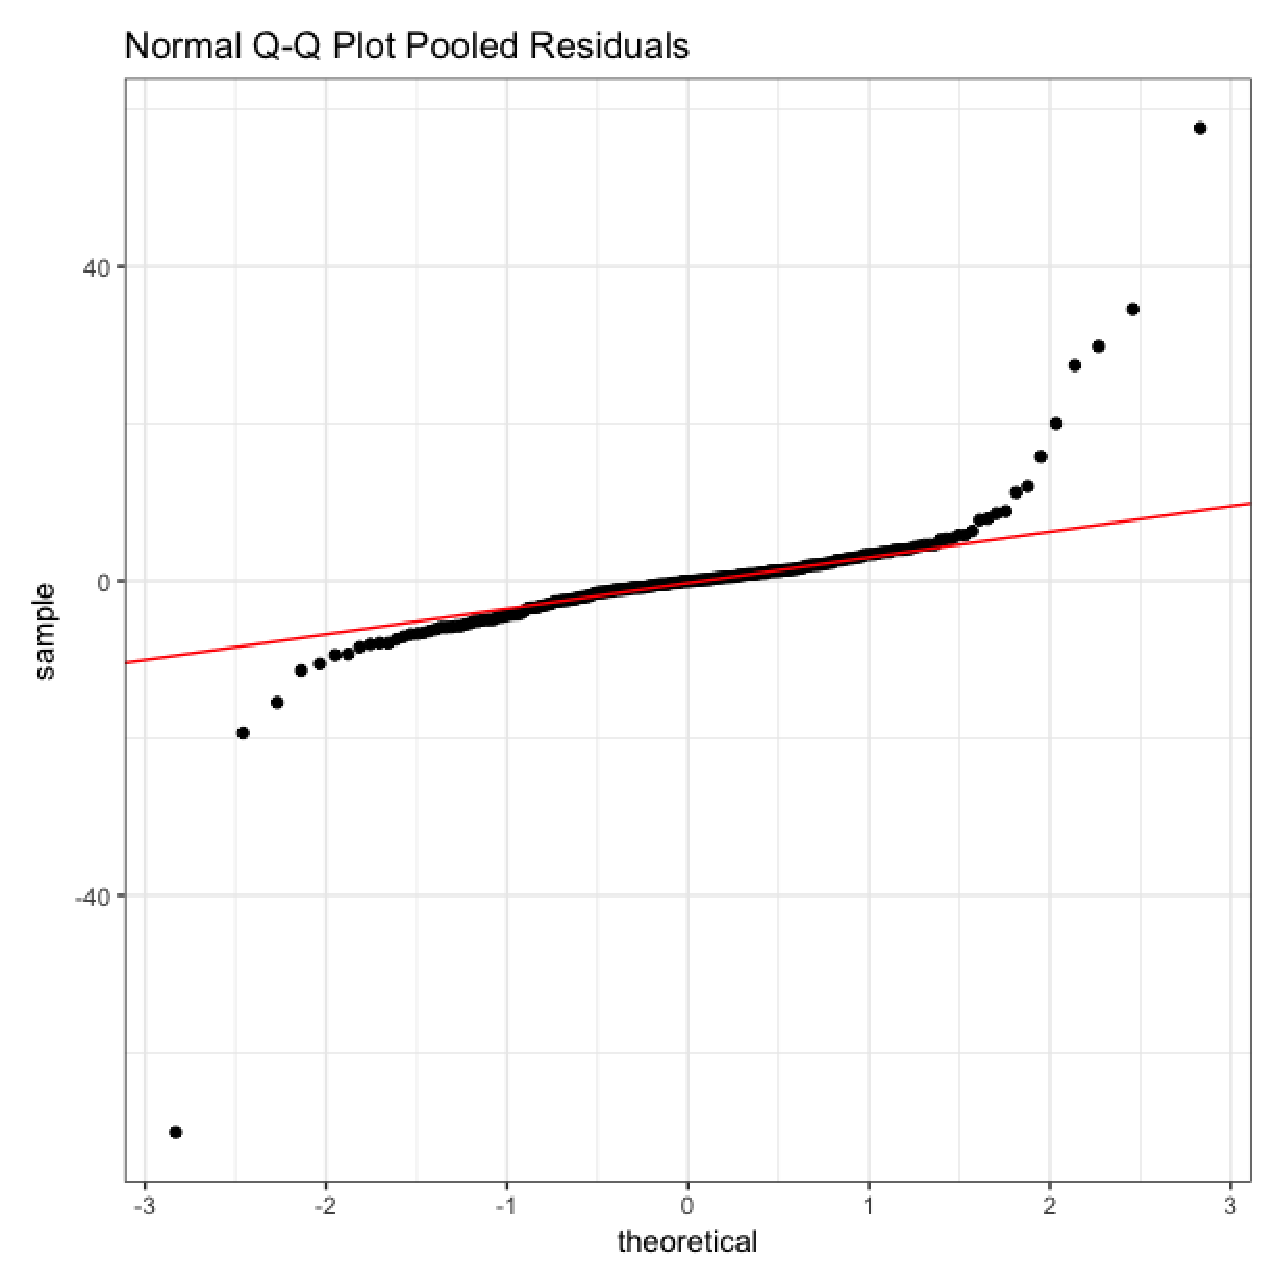
\includegraphics[scale=0.3]{picture/L16B_QQPool}$\quad$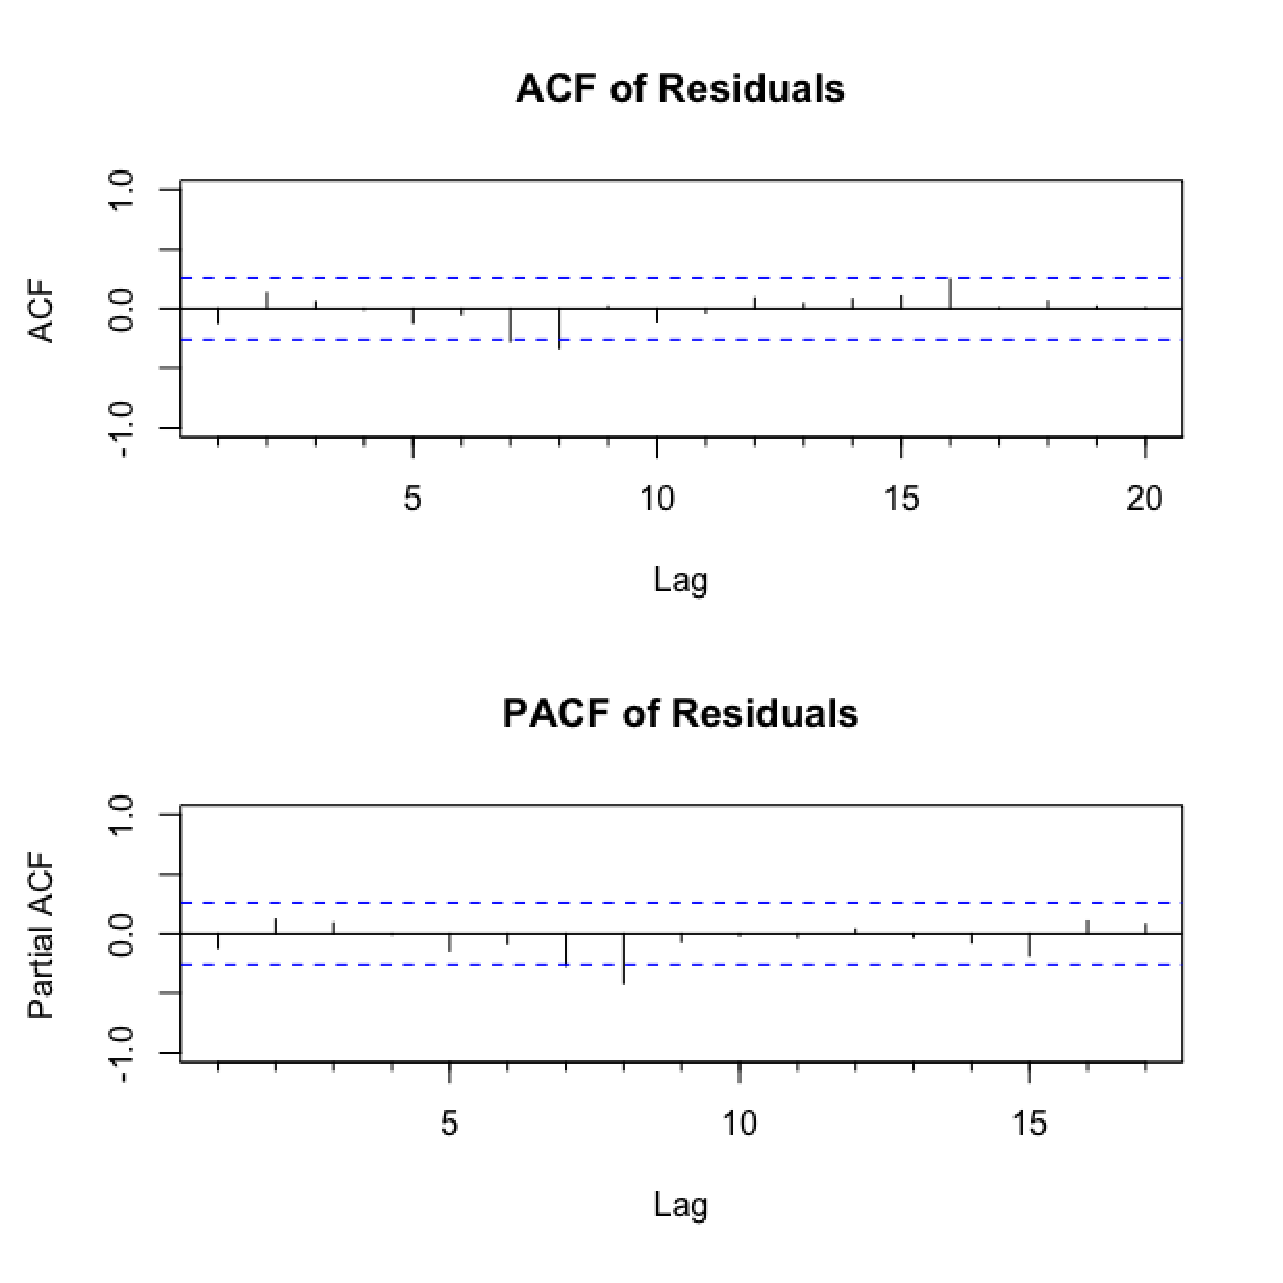
\includegraphics[scale=0.3]{picture/L16B_ACFPool}
\par\end{centering}
\caption{The normal Q-Q plot and the ACF/PACF of pooled residuals of the software
release B}
\label{L16B_plotDiag}
\end{figure}


\subsection{Software release C}

The Q-Q plot in \ref{L17A_plotDiag} suggests that a distribution
of the pooled residuals may have a tail thicker than that the one
of a normal distribution. It is visible that there are many extreme
positive and negative residuals in the plot. Furthermore, both the
ACF and PACF plots of pooled residuals are significant for the first
two lags. 

\begin{figure}[H]
\begin{centering}
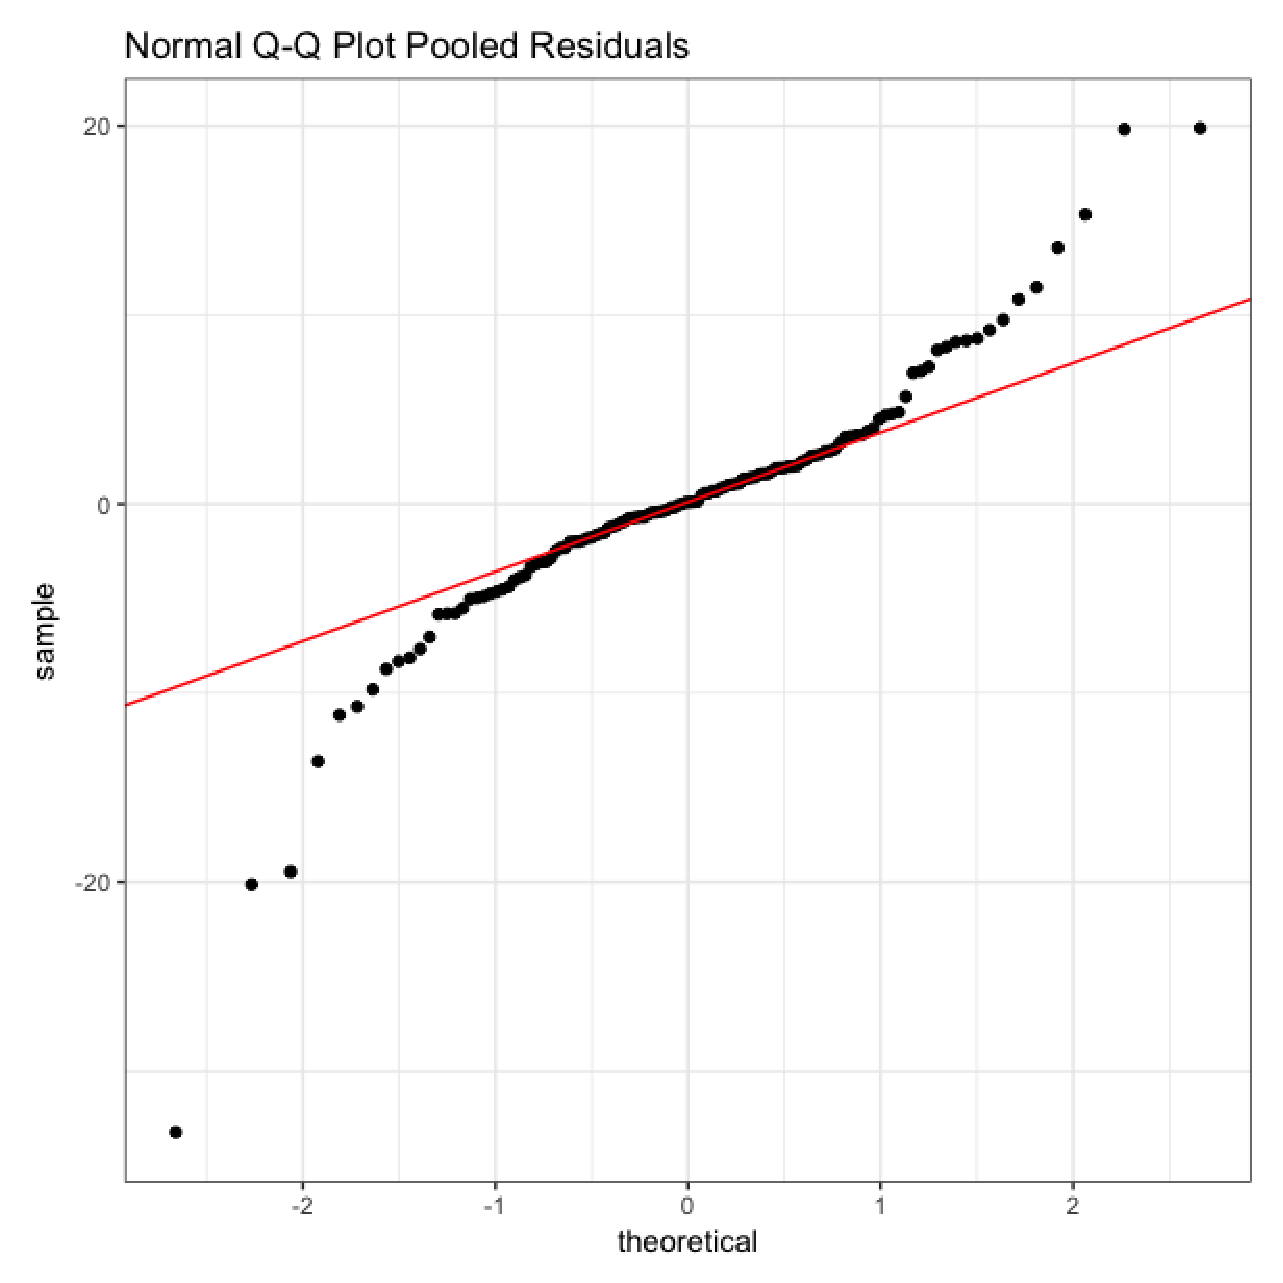
\includegraphics[scale=0.3]{picture/L17A_QQPool}$\quad$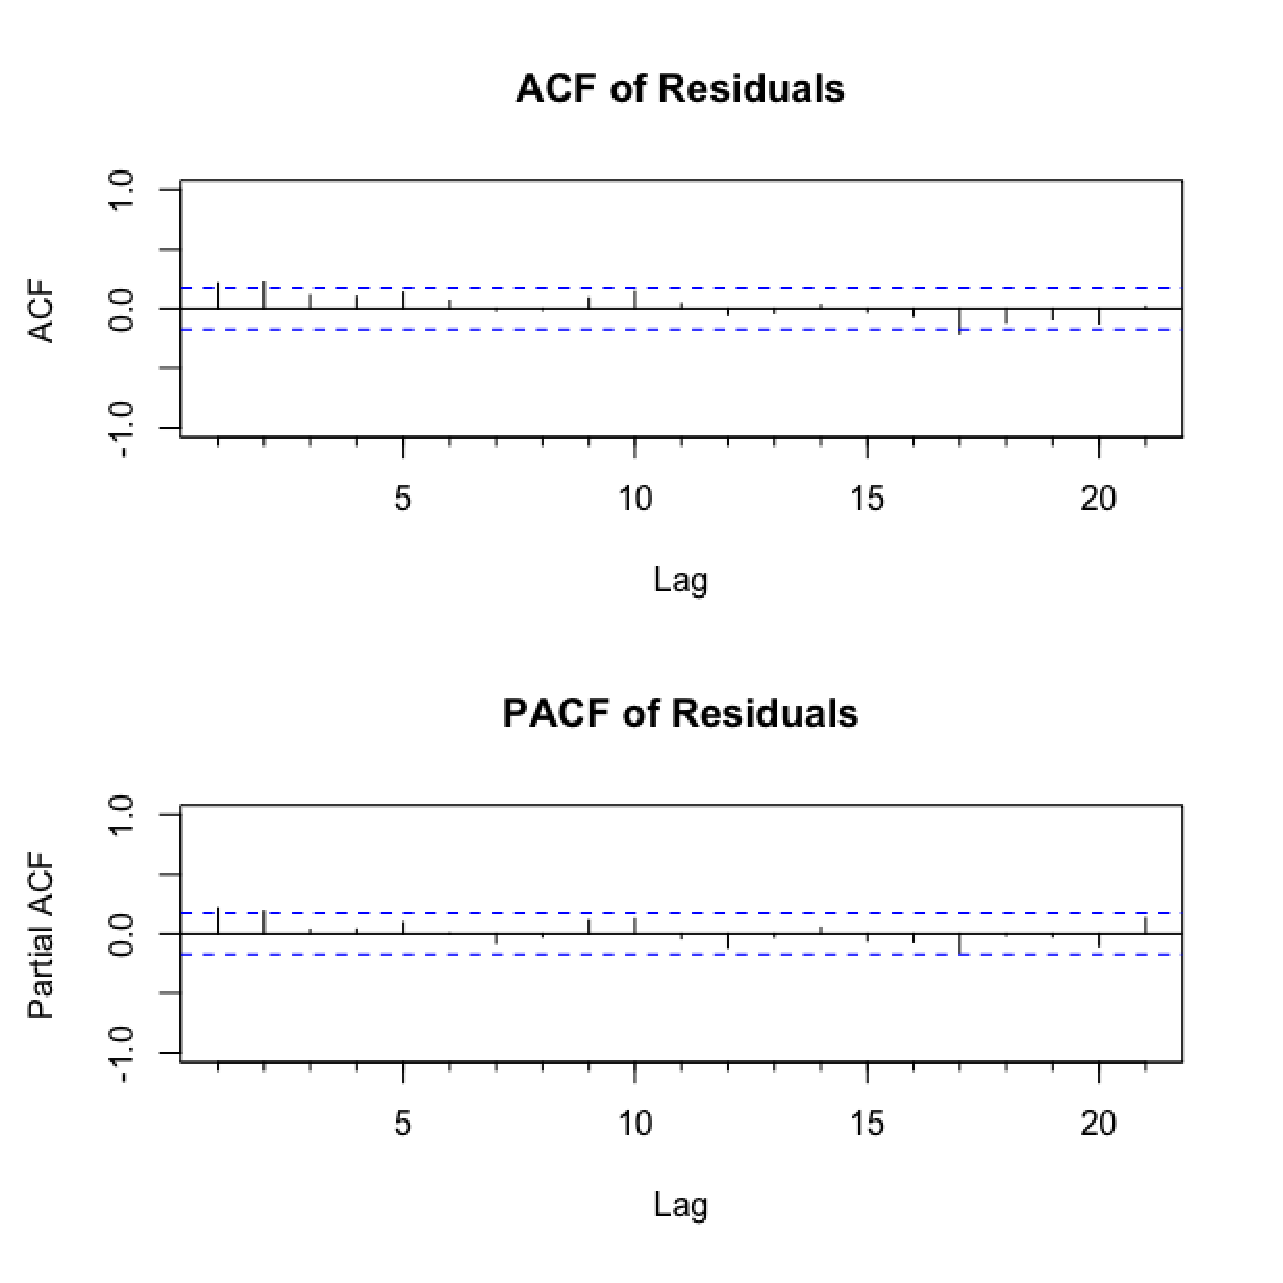
\includegraphics[scale=0.3]{picture/L17A_ACFPool}
\par\end{centering}
\caption{The normal Q-Q plot and the ACF/PACF of pooled residuals of the software
release C}
\label{L17A_plotDiag}
\end{figure}


\section{Non-parametric analysis}

An E-divisive method was applied to all three datasets. The method
reported one cluster for the dataset of the software release A and
five clusters for the dataset of each software release B and C. \ref{ediv}
shows places in the time series data where the E-divisive method detected
the significant changes. There is no estimated change point location
for the dataset of the software release A.

\begin{table}[h]
\caption{The locations of the statistically significant change points from
applying the E-divisive algorithm in each dataset}
\label{ediv}
\centering{}%
\begin{tabular}{cl}
\toprule 
Software release & Change-point location\tabularnewline
\midrule
\midrule 
A & -\tabularnewline
B & 130, 135, 153, 170\tabularnewline
C & 9, 77, 82, 105\tabularnewline
\bottomrule
\end{tabular}
\end{table}

The CPU utilization of the software release A, B and C along with
its estimated change points in the time series are plotted and shown
later in \ref{subsec:Real-data}. 

\section{Comparison between the Markov switching model and the E-divisive
method}

A comparison between the Markov switching model and the E-divisive
method was made in this section. These two methods were applied to
two simulated datasets, where the actual changes are already known
beforehand, and then also applied to a real data.

\subsection{Simulated Dataset 1}

\ref{compare_sim1} illustrates that the simulated data contains nine
estimated change point locations. For the Markov switching model,
the model reported two extra locations. The plot illustrates that,
besides the extra detected, the model performs rather well, as the
model discovers all the changes accurately. Only one change point
location was indicated to occur later than its actual occurrence time.
In contrast, the E-divisive method detected fewer changes than the
number of actual changes in the data. Furthermore, most of the detection
are also not quite accurate as three out of six detections are delayed
and one out of six detections is indicated to happen prior to its
actual time. The E-divisive method is unable to detect any changes
in the data at the beginning of the time period.

When these two methods detect changes after the actual changes, most
of their estimated change point locations are only behind by one or
two time index. To sum up, from this dataset, the Markov switching
model had more false alarms while the E-divisive had more missed detections. 

\begin{figure}[h]
\begin{centering}
\includegraphics[scale=0.35]{picture/compare_sim1}
\par\end{centering}
\caption{The simulated Dataset 1 showing the estimated change point locations
indicated by dashed vertical lines from the Markov switching model
(Middle) and the E-divisive method (Bottom). The actual change point
locations in the data are indicated in the top plot. }

\label{compare_sim1}
\end{figure}


\subsection{Simulated Dataset 2}

\ref{compare_sim2} presents estimated change point locations of the
Markov switching model, the E-divisive method, and the actual change
points in the data. The simulated dataset contains numerous switches
between states. Generally, the Markov switching model is able to identify
the changes considerably well despite a few false alarms and missed
detections. On the other hand, the E-divisive method can detect only
two estimated change points. Both two detections were correctly located.
The method has quite poor performance as it failed to detect most
of the change points in the data. The difference can be seen in the
plot.

\begin{figure}[H]
\begin{centering}
\includegraphics[scale=0.35]{picture/compare_sim2}
\par\end{centering}
\caption{The simulated Dataset 2 showing the estimated change point locations
indicated by dashed vertical lines from the Markov switching model
(Middle) and the E-divisive method (Bottom). The actual change point
locations in the data are indicated in the top plot. }

\label{compare_sim2}
\end{figure}


\subsection{Real data \label{subsec:Real-data}}

\subsubsection{Software release A}

According to \ref{ediv}, the E-divisive method could not identify
any changes in the dataset of the software release A. Thus, a comparison
between two methods could not be made for this dataset. 

\begin{figure}[H]
\begin{centering}
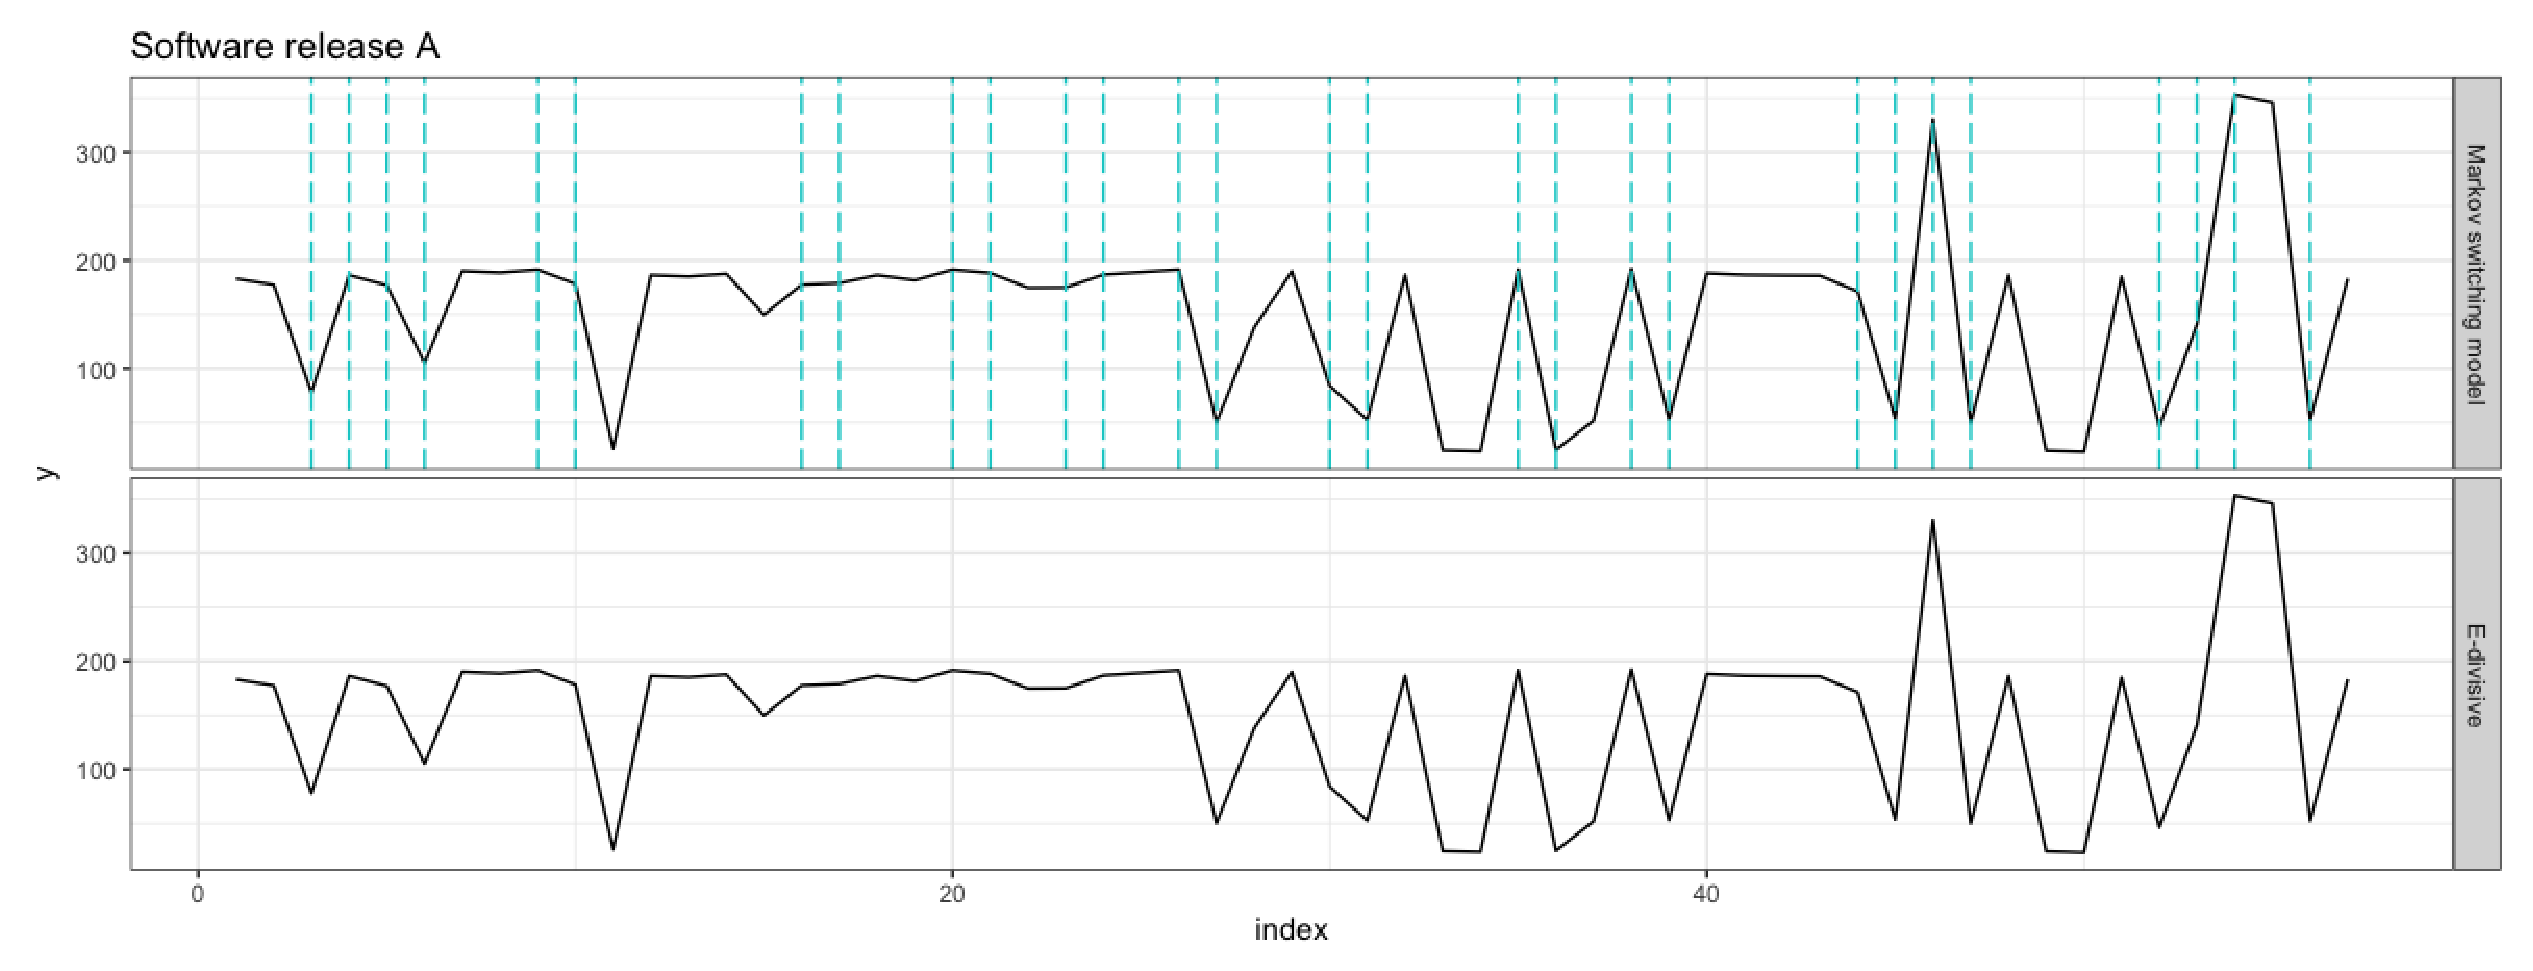
\includegraphics[scale=0.35]{picture/compare_L16A}
\par\end{centering}
\caption{The CPU utilization of the software release A. The dashed vertical
lines indicate the locations of estimated change points from the Markov
switching model (Top). }

\label{compare_L16A}
\end{figure}


\subsubsection{Software release B}

\ref{compare_L16B} presents results of estimated change points from
the Markov switching model and the E-divisive method for the software
release B. Sixty-three estimated change point locations are found
by the Markov switching model. On the contrary, only four estimated
change point locations are identified from the E-divisive method.
They are likely to occur around the same period of time. Most of the
locations of the change point detected by the E-divisive method are
at positive and negative peaks. Apparently, only one change point
location is determined at the exact same time from both methods, and
two change points are closely located. The rest of the detected locations
are completely different for each method.

\begin{figure}[H]
\begin{centering}
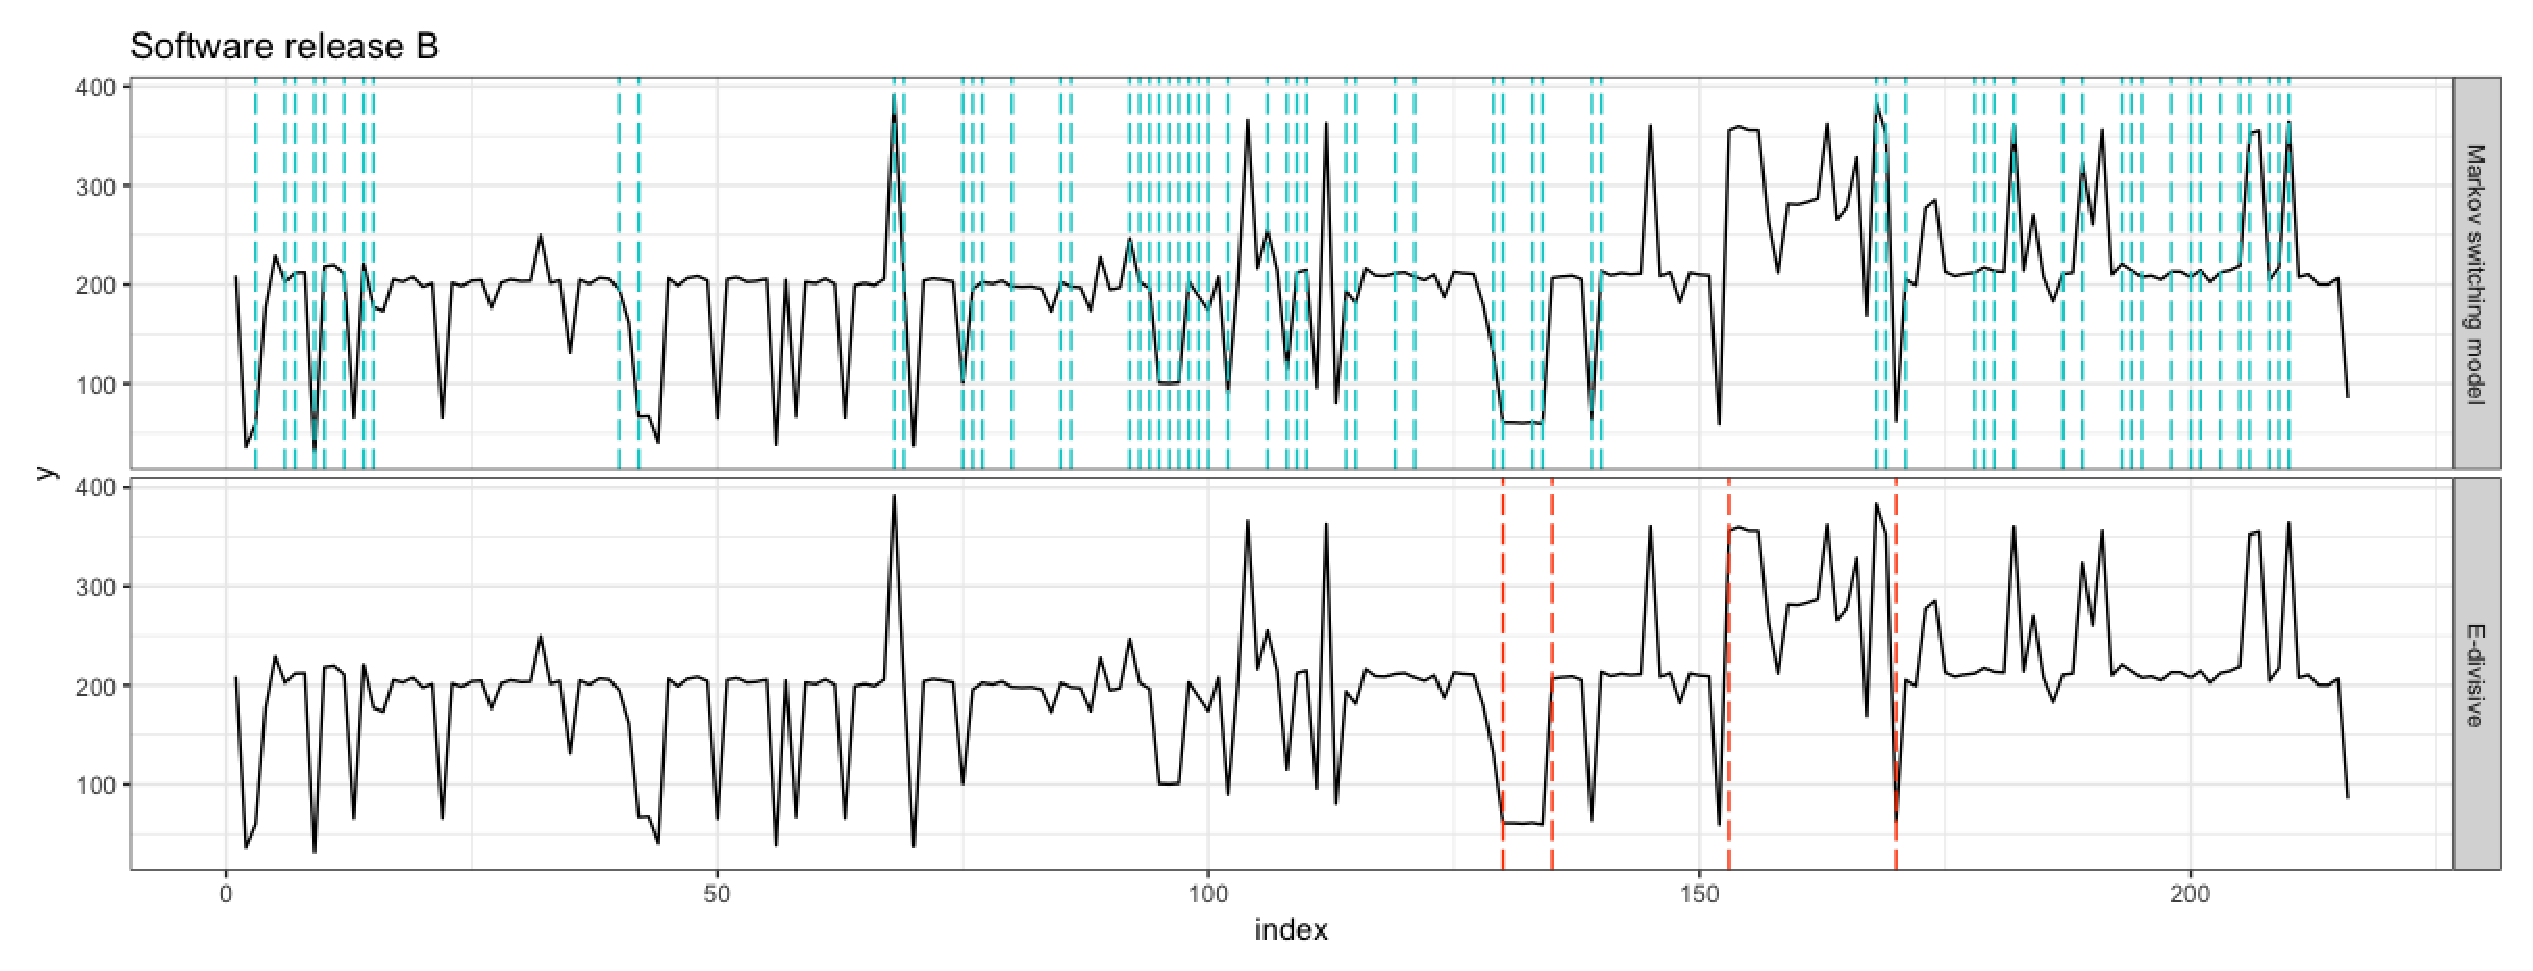
\includegraphics[scale=0.35]{picture/compare_L16B}
\par\end{centering}
\caption{The CPU utilization of the software release B. The dashed vertical
lines indicate the locations of estimated change points from the Markov
switching model (Top) and the E-divisive method (Bottom). }

\label{compare_L16B}
\end{figure}


\subsubsection{Software release C}

For the software release C, thirty-seven changes were discovered by
the Markov switching model as can be seen in \ref{compare_L17A}.
However, only four change point locations were identified from the
E-divisive method. These locations are rather spread out if compared
to the results from the software release B. The E-divisive method
discovered changes when the CPU utilization value was about to decrease
or increase. From both methods, two change points are determined at
exactly the same locations, and another one which is located in the
beginning is close to one another. Other detect locations are totally
different as shown in the plot. 

\begin{figure}[H]
\begin{centering}
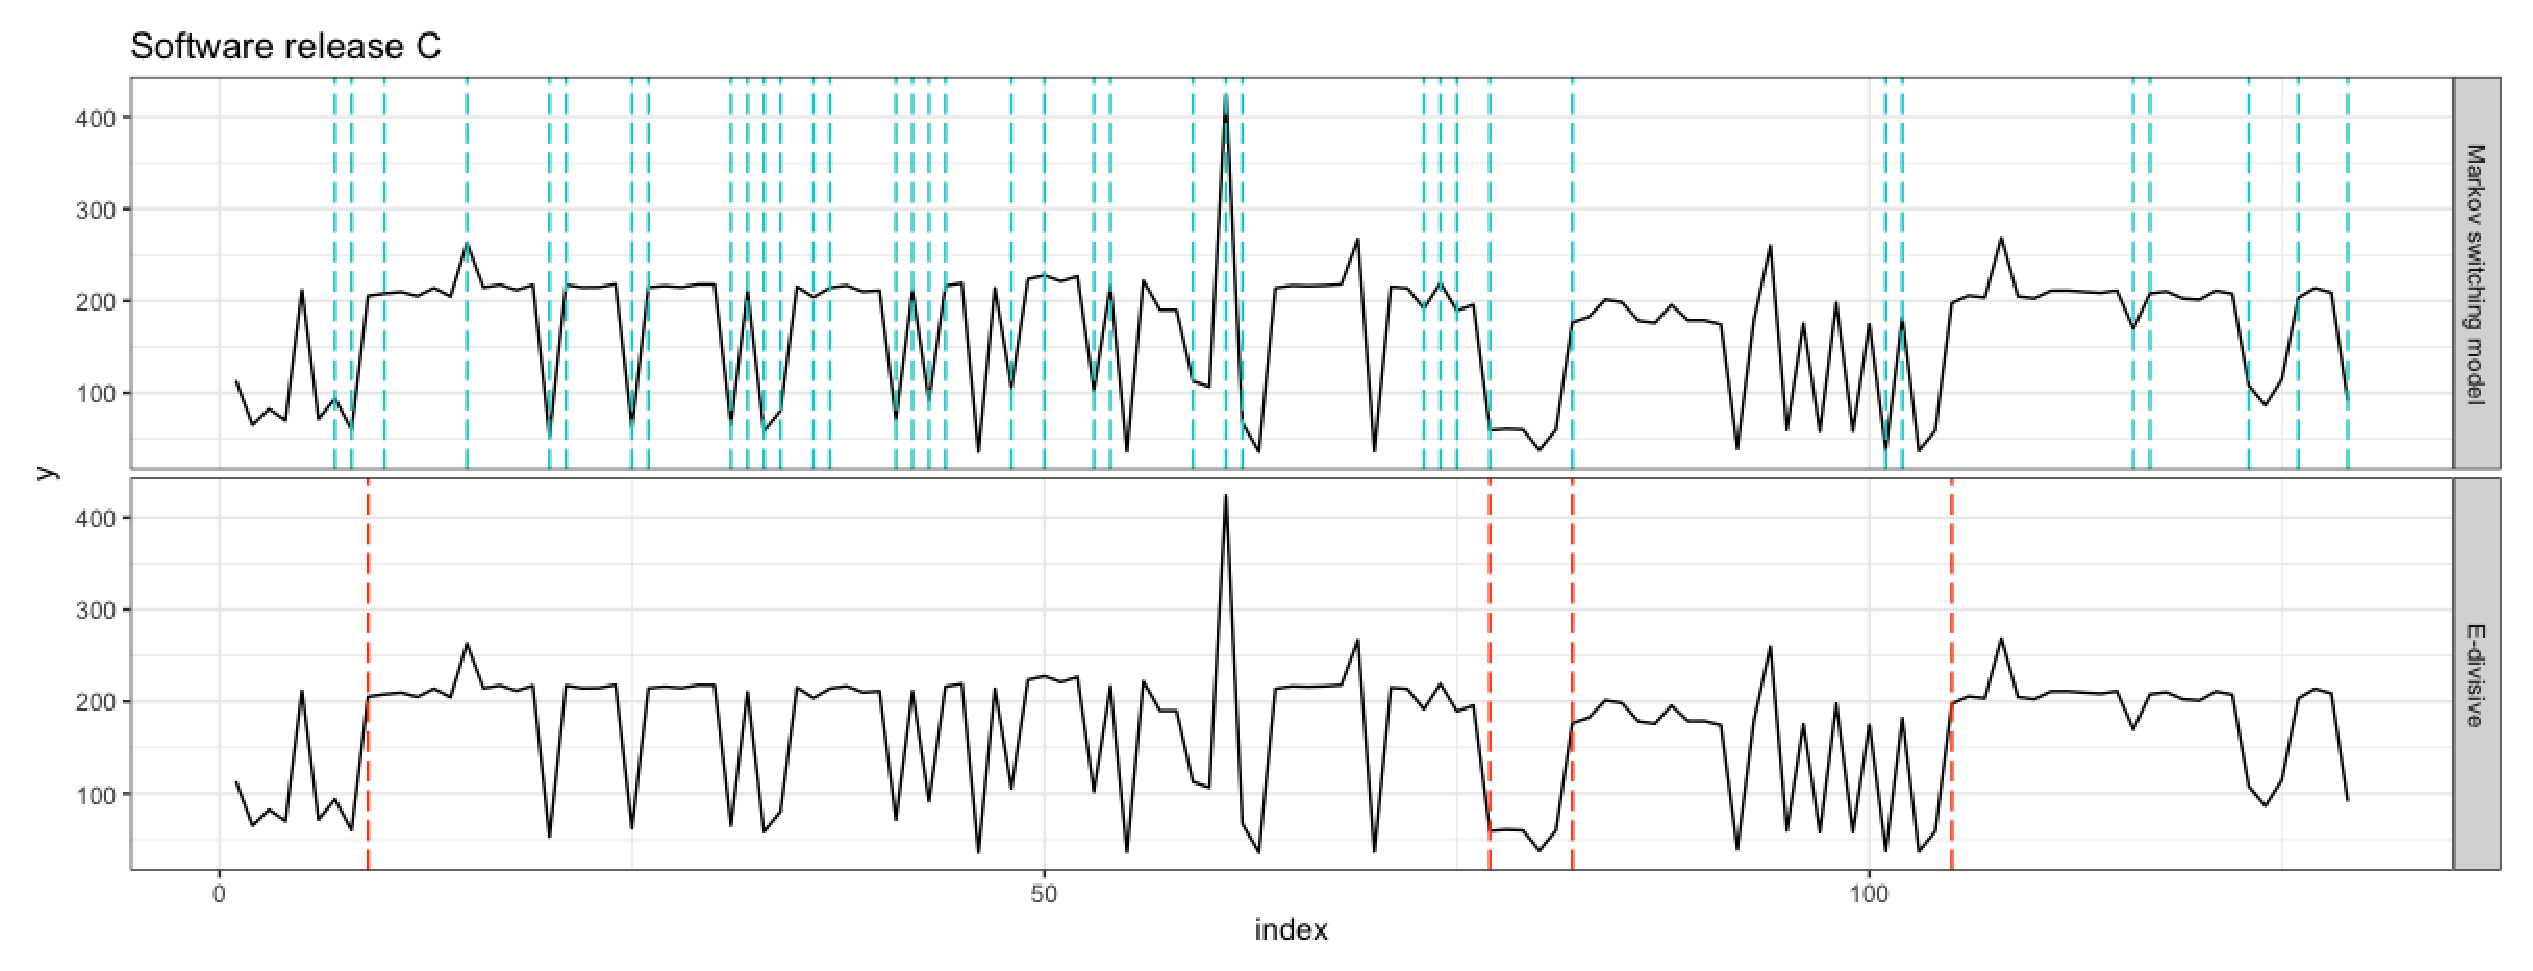
\includegraphics[scale=0.35]{picture/compare_L17A}
\par\end{centering}
\caption{The CPU utilization of the software release C. The dashed vertical
lines indicate the locations of estimated change points from the Markov
switching model (Top) and the E-divisive method (Bottom). }

\label{compare_L17A}
\end{figure}


\section{Predicting the state of the CPU utilization \label{sec:Predict}}

In this section, the state prediction function was implemented to
the test set in order to predict the most probable state for new observations. 

\subsection{Software release A}

For the software release A, there are 7 observations in total. In
\ref{predict_L16A}, only two states, State1 and State2, are assigned
for these observations. The first three observations are in State2.
Afterwards, the observations tend to switch back and forth between
both states until the end of the time period. Note that the most likely
state for the last observation of the test set is unable to be predicted,
and so it does not belong to any state.

\begin{figure}[h]
\begin{centering}
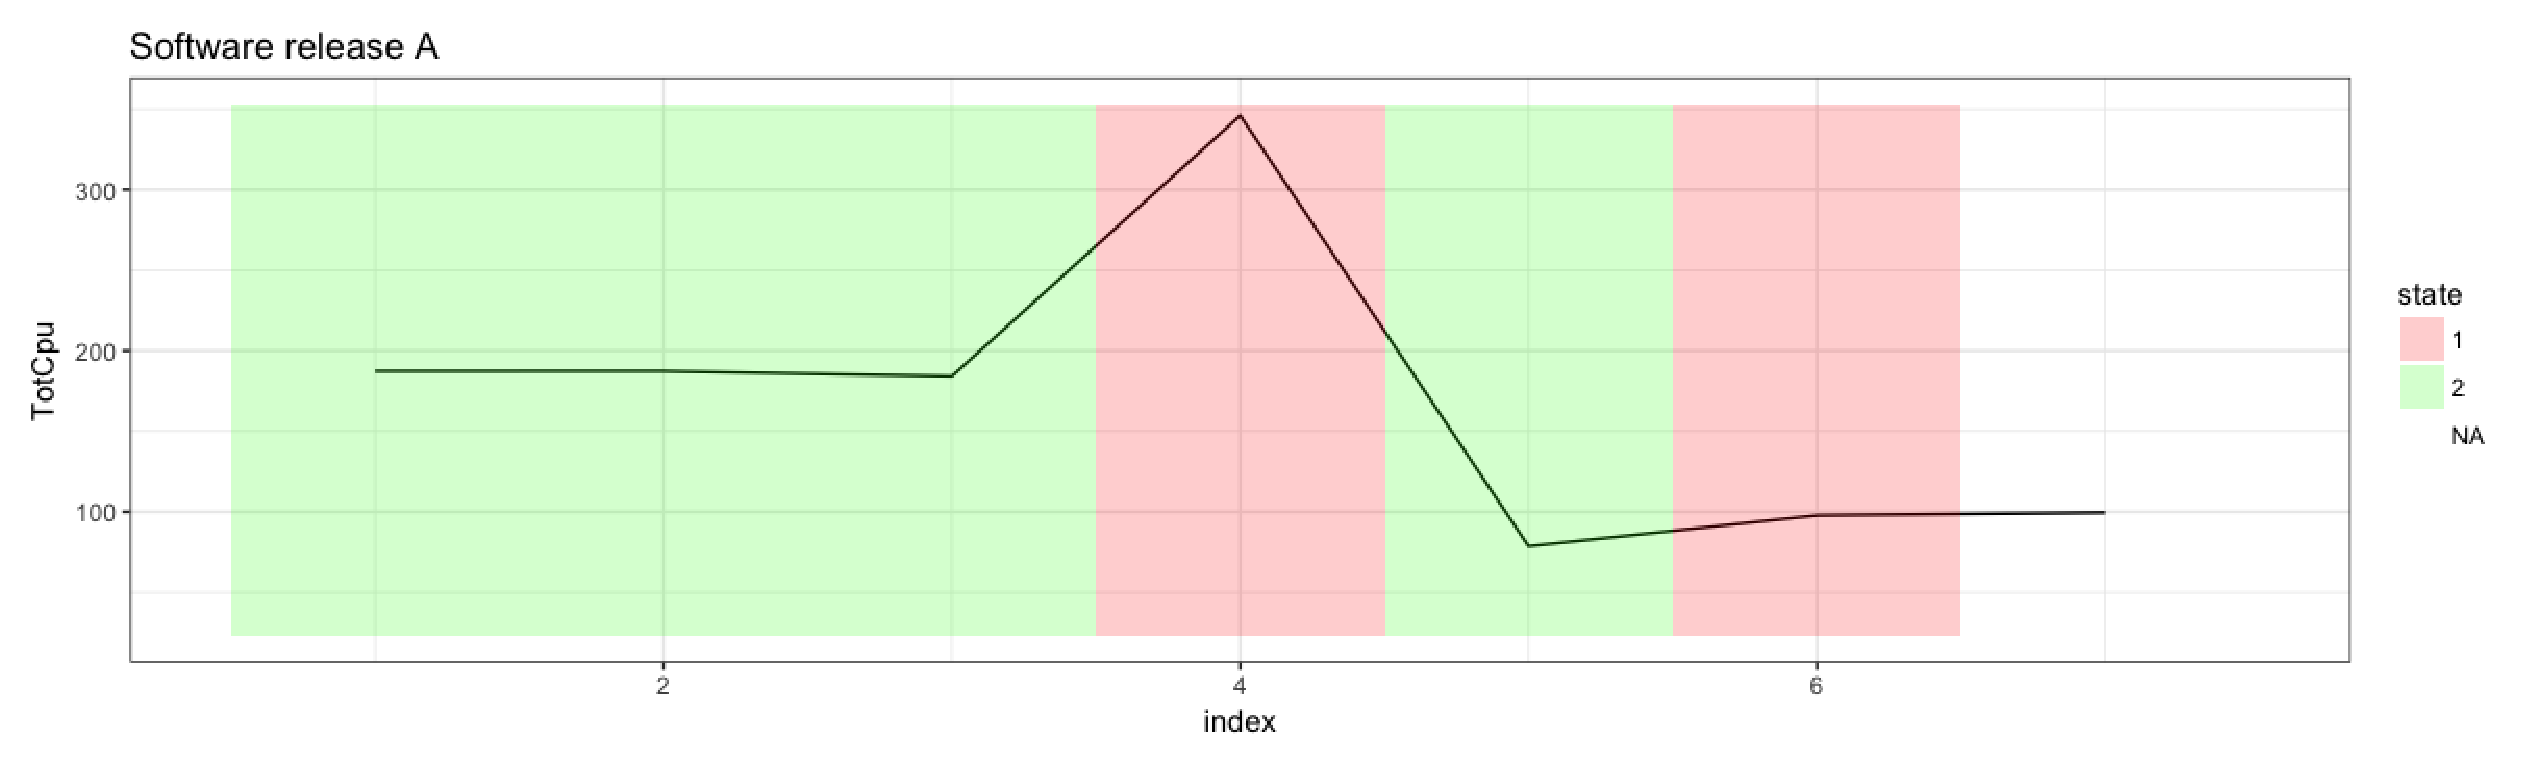
\includegraphics[scale=0.35]{picture/predict_L16A1}
\par\end{centering}
\caption{The predicted state of the test set in the software release A }

\label{predict_L16A}
\end{figure}


\subsection{Software release B}

In total, there are 25 observations in the test set of the software
release B. The result after applying the predict function to the test
set is shown in \ref{predict_L16B}. Observation 15 is the only observation
which is in State2. Many switches between State1 and State2 can be
seen from the plot. In addition, observation appears to stay in State1
only a short time before moving to State3, except for the first five
observations. 

\begin{figure}[h]
\begin{centering}
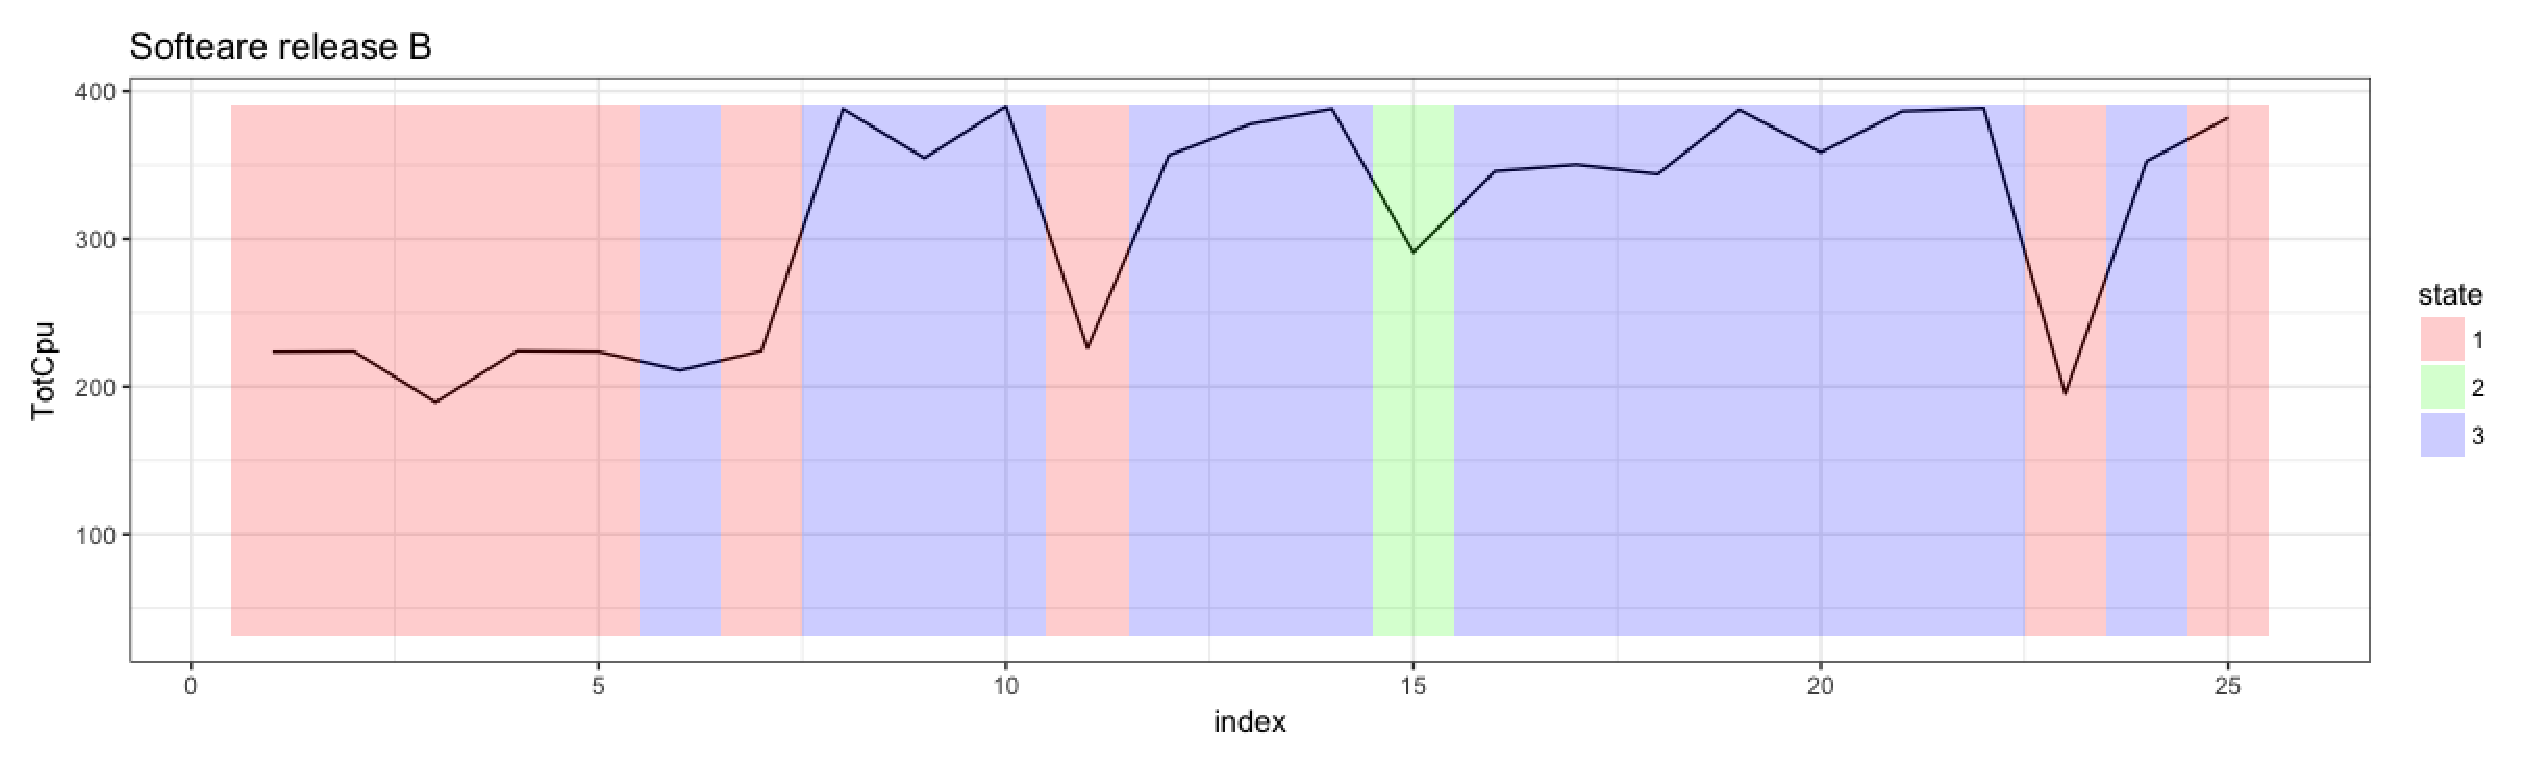
\includegraphics[scale=0.35]{picture/predict_L16B1}
\par\end{centering}
\caption{The predicted state of the test set in the software release B}

\label{predict_L16B}
\end{figure}


\subsection{Software release C}

The test set of the software release C consists of 15 observations
in total. \ref{predict_L17A} illustrates that the observations stay
in State2 for a considerably long period of time (observation 10-15).
There are several switches between states shown in the plot. The time
period between the observations between 4 and 7 switch between states
rapidly. The observations visit a particular state for one time, and
then immediately move to the another state. 

\begin{figure}[h]
\begin{centering}
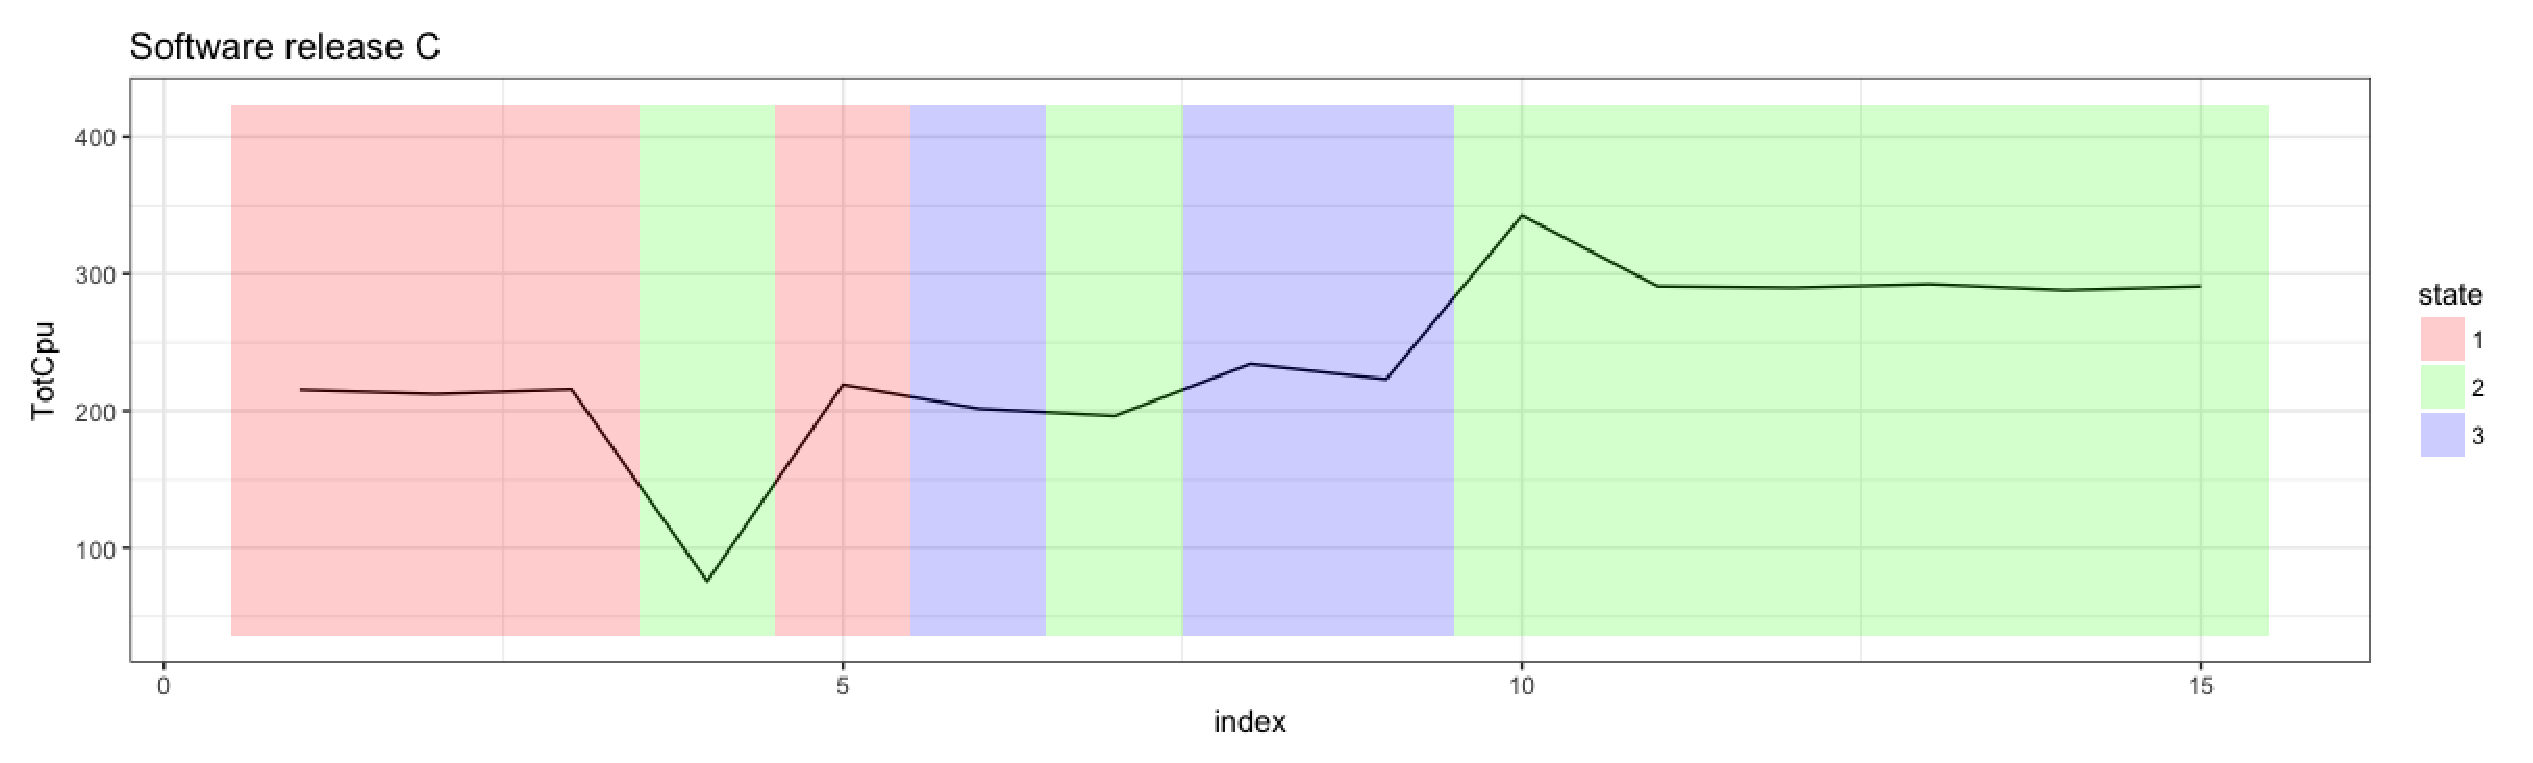
\includegraphics[scale=0.35]{picture/predict_L17A1}
\par\end{centering}
\caption{The predicted state of the test set in the software release C}
\label{predict_L17A}
\end{figure}


\section{Model evaluation \label{sec:Assessing}}

Eighty percents of the observations from the simulated data were fitted
with Markov switching model, and the remaining was used as a test
set to evaluate the performance of the model. 

\subsection{Simulated Dataset 1}

\ref{output-sim1} presents outputs from applying the Markov switching
model with the simulated Dataset 1. Each state has a considerably
high r-squared value which is greater than 0.9. From the results,
State2 has the highest standard error. When inferring back to the
actual models that were used to generate these three states in \ref{sec:Simulation},
it could be concluded that the result State1, State2, and State3 in
the table are a \emph{Bad}, \emph{Normal}, and \emph{Good} state,
respectively.

\begin{table}[H]
\caption{Outputs from applying the Markov switching model with the simulated
Dataset 1. The table shows estimated coefficients, residual standard
error, and r-squared for each state. A switching coefficient is followed
by (S), and a significant coefficient is highlighted in bold.}

\begin{centering}
\begin{tabular}{lr@{\extracolsep{0pt}.}lr@{\extracolsep{0pt}.}lr@{\extracolsep{0pt}.}l}
\toprule 
Estimated coefficient & \multicolumn{2}{c}{State 1} & \multicolumn{2}{c}{State 2} & \multicolumn{2}{c}{State 3}\tabularnewline
\midrule
\midrule 
(Intercept)(S) & \textbf{1}&\textbf{3024} & \textbf{5}&\textbf{5339} & \textbf{-14}&\textbf{3116}\tabularnewline
x1(S) & \textbf{0}&\textbf{8005} & \textbf{0}&\textbf{5900} & \textbf{0}&\textbf{7005}\tabularnewline
x2(S) & 0&0003 & \textbf{-0}&\textbf{8610} & \textbf{0}&\textbf{1941}\tabularnewline
y\_1(S) & \textbf{0}&\textbf{1902} & \textbf{0}&\textbf{3843} & \textbf{-0}&\textbf{1927}\tabularnewline
\midrule 
Residual standard error & 1&4900 & 7&3013 & 1&8255\tabularnewline
$r^{2}$ & 0&9980 & 0&9467 & 0&9962\tabularnewline
\bottomrule
\end{tabular}
\par\end{centering}
\centering{}\label{output-sim1}
\end{table}

The result of the model performance using Dataset 1 is shown in \ref{confusion}.
There are two observations from a \emph{Bad} state which were incorrectly
predicted to be in a Normal state. Moreover, two more observations
from a \emph{Good} state were predicted to be in a \emph{Normal} state.
The overall accuracy of the model is 0.96, and the misclassification
rate is 0.04. One can see that the model was able to perfectly predict
the state of the observations that are in a \emph{Normal} state. 

\begin{table}[h]
\caption{The confusion matrix of the result from the test set of the simulated
Dataset 1}
\label{confusion}
\centering{}%
\begin{tabular}{ccccc}
 & \multirow{1}{*}{} & \multicolumn{3}{c}{Predicted state}\tabularnewline
\cmidrule{2-5} 
 &  & Bad & Normal & Good\tabularnewline
\cmidrule{2-5} 
\multirow{3}{*}{Actual state} & Bad & 58 & 2 & 0\tabularnewline
\cmidrule{2-5} 
 & Normal & 0 & 30 & 0\tabularnewline
\cmidrule{2-5} 
 & Good & 0 & 2 & 8\tabularnewline
\cmidrule{2-5} 
\end{tabular}
\end{table}


\subsection{Simulated Dataset 2}

Outputs after applying the Markov switching model with the simulated
Dataset 2 are presented in \ref{output-sim2}. The r-squared values
of State1 and State3 are slightly lower than the obtained results
from the simulated Dataset 1, but the standard errors are significantly
higher. However, State2 has close output value to the simulated Dataset1.
It could be said that the model still performs rather well as the
r-squared value is very high. State1 is said to be a \emph{Bad} state
although an intercept is insignificant. State2 and State3 are a \emph{Good}
and \emph{Normal} state, respectively.

\begin{table}[H]
\caption{Outputs from applying the Markov switching model with the simulated
Dataset 2. The table shows estimated coefficients, residual standard
error, and r-squared for each state. A switching coefficient is followed
by (S), and a significant coefficient is highlighted in bold.}

\begin{centering}
\begin{tabular}{lr@{\extracolsep{0pt}.}lr@{\extracolsep{0pt}.}lr@{\extracolsep{0pt}.}l}
\toprule 
Estimated coefficient & \multicolumn{2}{c}{State 1} & \multicolumn{2}{c}{State 2} & \multicolumn{2}{c}{State 3}\tabularnewline
\midrule
\midrule 
(Intercept)(S) & 5&0716 & \textbf{9}&\textbf{0219} & \textbf{23}&\textbf{1711}\tabularnewline
x1(S) & \textbf{0}&\textbf{8672} & \textbf{0}&\textbf{5401} & \textbf{0}&\textbf{5546}\tabularnewline
x2(S) & -0&0195 & \textbf{0}&\textbf{2599} & \textbf{-1}&\textbf{1239}\tabularnewline
y\_1(S) & \textbf{0}&\textbf{1232} & \textbf{-0}&\textbf{0882} & \textbf{0}&\textbf{2272}\tabularnewline
\midrule 
Residual standard error & 6&6367 & 5&3211 & 7&5079\tabularnewline
$r^{2}$ & 0&9089 & 0&9480 & 0&9337\tabularnewline
\bottomrule
\end{tabular}
\par\end{centering}
\centering{}\label{output-sim2}
\end{table}

\ref{confusion2} presents a confusion matrix for a test set from
a second simulated dataset. The model was able to correctly predict
all the observations in a \emph{Bad} state. On the contrary, the model
did not perform well in predicting observations which had \emph{Good}
state. Nine observations from a \emph{Good} state were predicted to
be in a \emph{Bad} state, and another five observations from a \emph{Good}
state were inaccurately predicted to be in a \emph{Norma}l state.
Six observations from a \emph{Normal} state were incorrectly predicted
to be in a \emph{Good} state. The overall accuracy of the model and
the misclassification rate are 0.8 and 0.2, respectively. 

\begin{table}[h]
\caption{The confusion matrix of the result from the test set of the simulated
Dataset 2}
\label{confusion2}
\centering{}%
\begin{tabular}{ccccc}
 & \multirow{1}{*}{} & \multicolumn{3}{c}{Predicted state}\tabularnewline
\cmidrule{2-5} 
 &  & Bad & Normal & Good\tabularnewline
\cmidrule{2-5} 
\multirow{3}{*}{Actual state} & Bad & 35 & 0 & 0\tabularnewline
\cmidrule{2-5} 
 & Normal & 0 & 29 & 6\tabularnewline
\cmidrule{2-5} 
 & Good & 9 & 5 & 16\tabularnewline
\cmidrule{2-5} 
\end{tabular}
\end{table}





\lhead[\chaptername~\thechapter]{\rightmark}

\rhead[\leftmark]{}

\lfoot[\thepage]{}

\cfoot{}

\rfoot[]{\thepage}

\chapter{Discussion\label{chap:Discussion}}

In this chapter, a discussion of the model selection for each given
dataset is explained. Then, a state inference from the model is made.
Lastly, a results discussion of this study is provided.

\section{Model selection \label{subsec:Model-selection}}

In this analysis, a three-state model which had all switching coefficients
from Analysis I (see \ref{sec:States}) acted as a baseline model
for each dataset. This model was used to compare with other models
which had different combination of switching coefficients. If the
compared model has higher BIC than the baseline model, its performance
is concluded to be inferior and should not be considered for any further
analysis. However, only examining the BIC when choosing a model for
the data is insufficient. Remark that BIC might be unreliable for
a small or moderate dataset as BIC is derived under the assumption
of a normal distributed data \citep{ryden2008versus}. Therefore,
other aspects should also be taken into account along with the BIC
such as model outputs and plots. 

\paragraph*{Software release L16A}

Even though model 3 had the lowest BIC, a coefficient of \emph{Paging}
in one state had a zero standard error which led t-value to infinity.
This zero value can be interpreted as an actual zero or an extremely
small value that a computer treated as zero because significant digit
is lost. Nevertheless, either way suggests that this model is not
a good model to be used with this dataset as the model might be overfitting
with the training data. The standard error of zero means that there
is no variation in the data i.e., every data value is equal to the
mean value. Therefore, model 1 which had the second lowest BIC was
chosen for this given dataset instead. %
\begin{comment}
The t statistic is the coefficient divided by its standard error.
The standard error is an estimate of the standard deviation of the
coefficient, the amount it varies across cases. It can be thought
of as a measure of the precision with which the regression coefficient
is measured. If a coefficient is large compared to its standard error,
then it is probably different from 0.
\end{comment}


\paragraph*{Software release L16B}

Models 2 and 6 had the lowest BIC among the other models. Nonetheless,
their plots are similar to each other and provided a difficulty in
interpreting results (see \ref{L16B_NNY}). Observations stay in State3
in the first half of the period but stay in State2 in the second half
of the time period. There are continuous fluctuations of the CPU utilization
value through out the whole time period. Therefore, for observations
(or software packages) to remain in the same state for a long duration
without switching to other states seem unrealistic. The selected model
for this dataset was model 4 where its BIC was in the third lowest
place. Even though model 4 had slightly higher BIC than models 2 and
6, the model produced more sensible result.

\paragraph*{Software release L17A}

\begin{comment}
Model 1 appeared to have a good model output and plot when comparing
with the rest of the models. 
\end{comment}
The first four models with lowest BIC (Models 1, 5, 3, and 7, respectively)
had similar results both in model outputs and plots.%
\begin{comment}
explanation when examining its plot.
\end{comment}
{} Thus, Model 1 which had the lowest BIC was chosen for this dataset.

\section{State inference}

Another important task after the suitable model was decided is to
make an inference on the derived states because the model output does
not provide any definition of these states. %
\begin{comment}
A function from the package will estimate coefficients in each state
without providing the definition of these states. 
\end{comment}
Therefore, an interpretation and inference of the state need to be
specified. The state inferences for each dataset are shown below. 

\paragraph{Software release L16A (see \ref{L16A_NN})}

\begin{comment}
\begin{itemize}
\item State1

Despite periods where there is a slightly decrease in CPU utilization
value, State1 contains two peaks which have the value of the CPU utilization
higher than 300. This clearly implies that test cases in State1 perform
badly and  is defined as a \emph{Degradation} state. 
\item State2 

The state appears to be an \emph{Improvement} state as there are many
periods where test cases have low value in the CPU utilization.
\item State3 

The performance for test cases in this state can be viewed as a \emph{Good}
state as well. However, State2 seems to capture the period where test
cases have lowest values better than State3, and State3 has two periods
of increasing to higher CPU utilization values. The state is, therefore,
said to be a \emph{Steady} state.
\end{itemize}
\end{comment}

Despite periods where there is a slightly decrease in CPU utilization
value, State1 contains two peaks which have the value of the CPU utilization
higher than 300. This clearly implies that test cases in State1 perform
badly and should be defined as a \emph{Degradation} state. As for
State2 and State3, both can be viewed as an Improvement state. However,
State2 seems to have many periods where test cases drop to a lower
value in the CPU utilization. State3 also has two periods of abrupt
change to higher CPU utilization values. Therefore, State2 appears
to be an \emph{Improvement} state while State3 is said to be a \emph{Steady}
state.

\paragraph*{Software release L16B (see \ref{L16B_NYY})}

\begin{comment}
\begin{itemize}
\item State1 

There are many high peaks occur in this state. Moreover, test cases
tend to increase the value of the CPU utilization when they remain
in the state. A \emph{Degradation} state is adequate for defining
behavior in this state.
\item State2 

The state could be characterized as an \emph{Improvement} state. A
decreasing pattern of the CPU utilization value can be seen in most
of the period.
\item State3 

The CPU utilization value for test cases in this state are either
high or low. The state contains the period of positive and negative
peaks and does not appear to have a specific characteristic for the
state of the CPU. For this reason, the state is said to be a \emph{Steady}
state.
\end{itemize}
\end{comment}

There are many high peaks occur in State1. Moreover, test cases tend
to increase the values of the CPU utilization when they enter this
state. Hence, State1 is said to be a \emph{Degradation} state. State2
could be characterized as an \emph{Improvement} state. The reason
for this is because a decreasing pattern of the CPU utilization value
for the test cases in State2 can be seen in most of the period. The
test cases which are in State3 have either high or low in the CPU
utilization value. State3 contains the period of positive and negative
peaks, and does not appear to have a specific characteristic for the
state of the CPU. The difficulty of making an interpretation for State3
infer that the state may be defined as a \emph{Steady} state.

\paragraph{Software release L17A (see \ref{L17A_NNN})}

\begin{comment}
\begin{itemize}
\item State1 

There a \emph{Degradation} state
\item State2 

Most of observations in the state have a decreasing pattern when enter
this state which is often comes from State1. As a consequence, an
\emph{Improvement} state is given for this state. 
\item State3 

The values of the CPU utilization for observations in the state have
an unclear pattern. The value is quite fluctuate and because of this
behavior, the state is labeled as a \emph{Steady} state. There is
a peak in the time series data which is viewed as an anomaly in this
case. 
\end{itemize}
\end{comment}
{} Sudden change in State1

Even though the values of the CPU utilization which stay in State1
drop in some periods, there is an increase in the CPU utilization
values in most of the periods. Hence, State1 could be defined as a
\emph{Degradation} state. The CPU utilization values clearly decrease
when test cases enter State2. These test cases often switch from State1,
which is thought to be a state where the performance of the test cases
perform badly. As a consequence, this behavior indicates an improving
in the test cases. Thus, State2 is defined as an \emph{Improvement}
state. On the contrary, the values of the CPU utilization for the
test cases in State3 have an unclear pattern. The values are quite
fluctuate and because of this behavior, the state is labeled as a
\emph{Steady} state. State3 also contains a peak which occur in the
time series data. This peak is viewed as an anomaly in this case. 

\section{Results discussion\label{sec:Results-discussion}}

A thorough search of relevant literature yielded that this thesis
work might be the first time that Markov switching model has been
applied to the data of CPU utilization. In previous works, this model
was mainly applied with financial data or signal processing which
were used as an inspiration for this study. However, because of differences
in the characteristic of data, the procedure was slightly adjusted.
\begin{comment}
A large amount of time was spent on understanding the data, examining
which variables had a significant impact on the CPU utilization, and
determining which methods would provide the best possible outcome
for this problem. Besides, after deciding on the most promising method,
a lot of effort was invested studying implemented algorithms in the
R package as well as modifying code as necessary. 
\end{comment}

In this study, \emph{NodeName}, which is used to execute test cases,
was assumed to be indifferent i.e., performance of test cases are
the same regardless of the machine. Therefore, selecting a minimum
value of the CPU utilization of the test case for each software package
in data preprocessing step is reasonable. 

\begin{comment}
Above all, one has to understand and accept a risk when deciding on
the number of states as there is no guarantee how many states would
yield the best outcome. This risk is also applied to a situation when
determining the number of switching coefficients in the model. 
\end{comment}
There is no fixed rules in deciding the number of states. Therefore,
difference number of states were tried with the method in order to
determine which number would be best for this analysis. The results
from the model with two states offered less details and did not cover
all happening situations. Furthermore, all the graphs of the two-state
model are unrealistic and also difficult in interpret. %
\begin{comment}
had one state with a considerably long period and another state with
a very short period. There is a problematic interpretation when trying
to make a rough inference on the derived states.
\end{comment}
Despite higher BICs for the dataset of the software release L16B and
L17A, three-state model provides more interpretable plots and better
fit to the time series data. The four-state Markov switching model
for each software release was also briefly tested in the analysis.
Apparently, defining four states caused more difficulty when fitting
the model and making an inference on the states. The results were
rather poor when compare to the model with two and three states and
was not include in the report. Higher number of states are more likely
to give worse results and were not considered. Thus, the number of
chosen states after applying Markov switching model to each dataset
was three. 

Among all the predictor variables, the local events variables in \emph{EventPerSec}
is more essential than the test environment variables. Having a constant
value for the local events variables would be inadequate to characterize
the whole time series data and its evolution. However, the test environment
variables do not necessarily require a switching mechanism. This is
why in this study, the test environment variable was possible to not
have a switching effect. %
\begin{comment}
In \ref{sec:Switching}, a hypothesis that the test environment variable
was possible to not have a switching effect was made. 

for each test case and should have flexible values in each of the
fixed number of state. Although these test environment variables affect
the CPU utilization, they do not need to have different values in
each state.
\end{comment}

Another thing worth mentioning is that when modeling the Markov switching
model, it is better to try estimating a simpler model first. The size
of the model grows exponentially according to the number of states
$k$, and the number of predictor variables $n$. In addition, if
all coefficients have switching effects, the model will have more
parameters to be estimated. The function in the package will try to
fit the model and estimate the value of the coefficients, but there
is no guarantee that the obtained results of the likelihood will be
a global maximum. As a consequence, the estimated values of the coefficients
cannot be completely trusted. \citet{perlin2015ms_regress} suggested
any model with $k>3$ and $n\geq4$ is not recommended. This is also
the main reason why not all the local events were included, and the
model was not made to have all the switching coefficients. 

As mentioned previously in \ref{sec:States}, a variable called \emph{DuProdName}
in the dataset of the software release L16A%
\begin{comment}
, which is an exact linear combination of the other variables,
\end{comment}
{} was excluded from the regression model as it caused a singularity
problem. %
\begin{comment}
The singularity often happens when the size of data is small. 
\end{comment}
This problem could be reduced by increasing the size of the data.
However, with a limited available data, fifty-seven observations in
this dataset, the variable \emph{DuProdName} has to be dropped from
the regression model before doing a further analysis. %
\begin{comment}
Fifty-seven observations in this dataset were used to train the Markov
switching model. The dataset (or the number of test cases in the software
release) is rather small, which increases a probability of singularity
occurrence. Therefore, unless there is more data, it is better to
drop the variable from the regression model before doing a further
analysis.
\end{comment}

For each software release, each state in the model has a significantly
high r-squared value which is greater than 0.9 (see \ref{chap:Output}).
R-squared value is an intuitive measurement to determine how well
the model fits with the data. In general, the higher r-squared value
is more preferable. Nevertheless, high r-squared value does not necessarily
indicate that the model is a good model because the model with high
r-squared value could be overfitting due to too many predictor variables
were used in the model. Using only r-squared value to determine adequacy
of the model can be misleading. A residual analysis should be considered
when evaluating a model. %
\begin{comment}
R-squared cannot determine whether the coefficient estimates and predictions
are biased, which is why you must assess the residual plots.

R-squared value cannot be solely used to indicate whether the model
is adequate or not. In order to assess this, a residual analysis is
required. 

There are many factors that affect value of r-squared. One factor
is the number of predictor variables in the model. R-squared value
increases when there are more terms in the model. Another reason,
which is somehow a consequence of adding too many predictor variables,
is that the model might be overfitting the data. As a result, the
model produces misleading high r-squared.
\end{comment}

A Q-Q plot is a visual check for an assumption of normality. The plot
provides a rough idea whether the assumption is plausible or not.
From the residual analysis in \ref{sec:Residual}, it revealed that
the residuals of all three datasets did not completely follow the
normal distribution. This is not surprising as real data rarely have
a well-defined structure. Since the Markov switching model assumed
normal distributed residuals, the chosen models might have less credible
results. In addition, the dataset used in this thesis is not sufficiently
large. As a result, the Q-Q plot is often unclear and difficult to
spot its basic feature due to more noises. ACF and PACF plots are
used to check a randomness in a data and also to identify a possible
structure of a time series data. The models of all three datasets
seemed to capture the dependent structure of the error terms in the
data, even though a small amount of autocorrelation were left in the
residuals. This suggests that the models could be slightly improved.
However, these plots indicate that using AR(1) is already justified
for these datasets. %
\begin{comment}
The assumption of a normally distributed residuals is justified for
software release L16B.

If the residuals appear to behave randomly, it suggests that the model
fits the data well.

randomness tends to obscure the actual behavior especially with small
data

Furthermore, the model is able to capture the pattern of data rather
well.

The model seems to capture the dependent structure of the error terms
in the time series, except for the reported significant lag. 

heavy tail = high variance

independent of noise terms

There is an outlier in the residuals (2004:Q4) which suggests there
was something unusual happening in that quarter. It would be worth
investigating that outlier to see if there were any unusual circumstances
or events that may have reduced beer production for the quarter.

The remaining residuals show that the model has captured the patterns
in the data quite well, although there is a small amount of autocorrelation
left in the residuals (seen in the significant spike in the ACF plot).
This suggests that the model can be slightly improved, although it
is unlikely to make much difference to the resulting forecasts.
\end{comment}

More importantly, the results of the Markov switching model could
be affected by various types of bias. Due to a small size of the training
data, the training model will not be very effective and unable to
capture the behaviors of new observations that lie outside the range
of the training data. %
\begin{comment}
For this reason, a prediction for the new observations might not be
accurate as it should be. 
\end{comment}
This could be seen in a state prediction of the software release L16A
(see \ref{sec:Predict}). Secondly, only the predictor variables that
have been analyzed to have significant impacts on the CPU utilization
were included in the model. However, many other variables that is
possible to have minor impact on the CPU utilization but were overlooked.
Therefore, there might be some bias by not including these variables
into the analysis. Finally, the criteria that has been used to select
the number of states and the number of switching coefficients in the
model are rather subjective. Hence, these chosen number might not
be the best for different perspectives and so could be counted as
one of the bias as well. %
\begin{comment}
other factors which are not considered in the model might also be
the reason of causing a bias. The chosen predictor variables in this
thesis are variables that have a partial prior knowledge and have
been analyzed to have some significant impacts on CPU utilization.
However, it is possible that there are still some explanatory information
that is overlooked. Finally, selecting the number of states and switching
coefficients in the model could cause a bias as well. Finally, selecting
the number of states and the number of switching coefficients in the
model could cause a bias as well. 
\end{comment}

As described above, the small dataset is proven to cause several problems
and difficulty to the analysis. The size of data is crucial in statistical
analysis because more information can be extracted and used as an
input for the model to learn. 

A benefit from using a non-parametric analysis is that it does not
require a prior assumption of a data distribution and is able to detect
any type of distributional change within a time series. One noted
behavior which can be seen from the results of the Markov switching
model and the E-divisive method in the simulated data is that if a
pattern of changing from one state to another state in the data is
not obvious, the E-divisive method will be unable to detect locations
of change points. For instance, the method could not identify any
changes in the first hundred observations, and also at the end of
the time series in the simulated Dataset 1. Besides, the duration
between states also affect the ability of discovering the change point
locations in the E-divisive method. To illustrate, the switching pattern
is considerably difficult to notice in the simulated Dataset 2. The
period of staying in the state is short and there are many switches
between states occur over the period of time. The shift for the response
variable is not dramatic that one can see the huge difference when
there is a switch in the state. Therefore, the E-divisive method could
only detect two change point locations where the shifts were obvious. 

After examining the results in both simulated datasets, the E-divisive
method proved to have less power in detecting changes in the data.
The E-divisive method and the Markov switching model appear to discover
changes at around the same time when the actual changes occur, despite
some false alarms and missed detections. This suggests that for the
real data where the actual state is unknown, the actual changes might
occur around locations where these two methods are able to detect.
In addition, there is a high probability to be an actual change of
the state if these two methods can identify the change point at the
exact same location.

Note that when performing a Markov switching model, variables which
have influences on the CPU utilization are also included in the model.
Nonetheless, the E-divisive method only considers the values of the
CPU utilization. With this difference, the E-divisive method will
have even less power to identify actual changes in the CPU utilization.
Since there are other variables that affect the value of the CPU utilization,
it is insufficient to take into account only the response variable.
\begin{comment}
The E-divisive method appears to perform reasonably well in detecting
changes as far as a non-parametric analysis could. As can be seen
from \ref{subsec:Real-data}, the method is able to detect when a
change is happened around the same time as the Markov switching model
did. Even though the E-divisive method might not provide the best
result, it can give a general idea of estimated change points.
\end{comment}

The state prediction function which is an additional implemented function
in the package seems to work properly. This can be observed by examining
the results from \ref{sec:Assessing}. The accuracy of the test set
in the simulated Dataset 1 was significantly high. One reason for
that might be because the simulated data had an obvious pattern in
switching between states. %
\begin{comment}
For example, the value of the CPU usage is moderately low if it is
generated from the Good state.
\end{comment}
Besides, each state remained in its own state for a while before switching
to the other states. Therefore, the model can completely capture the
behavior of the time series data. In contrast, the simulated Dataset
2 had several switches between states and each state did not have
a long duration. Even though the pattern of the response variable
is rather difficult to see in the plot, the Markov switching model
still perform rather well for this dataset.





\lhead[\chaptername~\thechapter]{\rightmark}

\rhead[\leftmark]{}

\lfoot[\thepage]{}

\cfoot{}

\rfoot[]{\thepage}

\chapter{Conclusions }

This thesis assesses an ability of detecting any changes in the performance
of the Ericsson's software products by applying the Markov switching
autoregressive model and the E-divisive method. The simulated datasets
with known states were used to make a comparison between both methods.
The results from applying the Markov switching model to the real data
were presented with interpretations and discussions. 

For the Markov switching model, the number of states and the number
of switching coefficients in the model were determined and chosen
by examining the BIC, along with model outputs and plots. The findings
from the simulated datasets revealed that the Markov switching model
were able to discover switches between states rather well, despite
some false alarms and missed detections. This method works well even
though numerous switches between states did occur in the data. The
E-divisive method is less powerful compared to the Markov switching
model. The method could identify fewer change point locations, and
failed to detect many changes that were occurred in the simulated
datasets. The E-divisive method will perform better and will be more
efficient if the data have an obvious pattern of shifting in the time
series. Based on the results from the simulated datasets and the real
data, the Markov switching model was considered to be the suitable
method for the analysis. The E-divisive method was rather used as
a guideline for any changes that could happen in the data. The method
could also be used together with the Markov switching model for a
confirmation of the changes in the data when the actual state is unknown.
After applying the Markov switching model to both simulated datasets,
the accuracy of the test sets implied that an implementation of a
state prediction function appears to work well. %
\begin{comment}
Moreover, an implementation of a state prediction function appears
to functionally work well when investigating on the simulated datasets.
The accuracy from both simulated datasets were high. 
\end{comment}

Evaluating the obtained results is rather difficult, mostly due to
a lack of annotations or label of the state of the CPU utilization.
This is a common situation to an unsupervised learning problem where
the ground truths are not often available. %
\begin{comment}
Besides, another difficulty of using the Markov switching model is
that a state inference is required. Since the Markov switching model
assumed latent states, a sensible inference is needed in order to
get a final and meaningful result that can be further used.
\end{comment}
To conclude, this work has provided knowledge to understand more about
the properties of the state of the CPU utilization which will, in
turn, pave the way for further analysis.

\section{Future work}

The Markov switching model gave quite promising results but several
improvements could also be done to increase the robustness of the
analysis. For future work, more extensive data is recommended. Obtained
results will be more reliable as additional information will decrease
an uncertainty in the data. %
\begin{comment}
As the assumption of the distribution of residuals was not entirely
fulfill, significant details that were used to explained the CPU utilization
might not all be caught by the model. Hence, another future extension
is to consider on the effects of interaction terms or the other predictor
variables, specifically local events in \emph{EventsPerSec}, that
might have an effect on the CPU utilization.
\end{comment}
{} 

Furthermore, there are still two more performance metrics in QA Capacity
area which have not been taken into account in the thesis i.e., memory
usage and latency. The analysis could also be extended to analyze
these metrics in a further work. 

Another future extension to get the best state prediction is to consider
applying the Markov switching autoregressive model on the different
QA Capacity test case types i.e., one model for each type of test
case. Results are expected to be more accurate as value of the CPU
utilization will be slightly more stable and not so fluctuating.

It would also be interesting to use normalized values by introducing
weight parameters instead of using the real value of the local events
in the \emph{EventsPerSec} and the CPU utilization. Different weights
can be given to the local events depending on how much effect it has
on the CPU utilization. These values are summed up and then divided
by the CPU utilization value to get a final value that represents
a value with respect to a specific type of test case and the CPU utilization.

Finally, in the future if some test cases have been labeled by an
area expert, a semi-supervised learning algorithm, a technique that
falls between supervised and unsupervised learning, could also be
implemented. Training a model with a large amount of unlabeled data
and a small amount of labeled data could considerably improve the
accuracy of the model. The semi-supervised learning could be of good
practical use, especially for applications where labeling all the
data is very expensive and time-consuming. 




\cleardoublepage{}


\appendix

\lhead[\chaptername~\thechapter]{\rightmark}

\rhead[\leftmark]{}

\lfoot[\thepage]{}

\cfoot{}

\rfoot[]{\thepage}

\chapter{Implementation in \emph{R}\label{chap:Implementation}}

\begin{comment}
Both R and Python are powerful programming languages for data analysis.
Python has been known as a general purpose language with an easy to
understand syntax. It emphasizes on code readability and has a gentle
learning curve. R is developed by and for statistician. It provides
a huge number of essential packages in statistics, and even starts
to expand its package to different fields. R also has a strong reputation
for data visualization. However, in terms of computation, R still
cannot compete with Python which is built specifically for the computer
programming. 

With strengths and weaknesses between R and Python described earlier,
R is chosen to be used in this study. R offers more implemented algorithms
to solve the problem at hand. Moreover, an effective visualization
helps analyst and user to understand more about their data especially
for the complex one. Visualizing data is useful in many ways such
as uncover new patterns, identify some factors, and get an overall
trend. R proves to be a good choice as it provides a great feature
in creating an interactive graphic.
\end{comment}


\section{EventsPerSec\label{sec:EventsPerSec}}

The \emph{EventsPerSec} variable contains several local events in
the test case which are separated by a tab character. A function to
split tab-separated values in the field into columns is described
by the following steps.

\begin{algorithm}[h]
\caption{Extract local events in EventsPerSec}

\begin{algorithmic}[1] 
\For{each test case}
\State{Split the vector of local events with its value into elements} 
\For{each element} 
\State{Split the element into the local event and the value}
\If{the column of the local event exists in the data}
\State{Insert value}
\Else{}
\State{Create new column for this local event and insert its value}
\EndIf
\EndFor
\EndFor
\State{Replace missing value with zero}
\end{algorithmic}
\end{algorithm}


\section{MSwM Package\label{sec:MSwM-Package}}

A \emph{MSwM} package in R \citep{mswm} is mainly used to perform
an univariate autoregressive Markov switching model for linear and
generalized models. The package implements an Expectation-Maximization
(E-M) algorithm to fit the Markov switching model. 

Code was further implemented, and some modifications were also made
in the function to handle warnings and errors produced when fitting
the model. These modifications are described in more details here.

\paragraph*{Non-switching effect}

When setting variance to have a non-switching effect, a function generates
a warning. This issue is caused by a minor mistake in the code. 

\paragraph{Non-invertible Hessian}

The package uses a Hessian, a matrix of second order partial derivatives
with respect to parameters, for a numerical optimization. In some
cases, the Hessian matrix will not be invertible as the matrix is
singular. Consequently, the function cannot compute the standard error
of estimated parameters. It is assumed that the singularity is coming
from numerics issue i.e., the matrix is not singular but computationally
it is. This non-invertible Hessian is solved by using generalized
inverse (or pseudoinverse) procedure \citep{gill2004your}. 

\paragraph*{Plots}

Two more plots for visualizing the results have been added to the
package. Name of functions and descriptions are provided below. 
\begin{itemize}
\item \code{plotSmo(object)} 

Plot of smoothed probabilities with different states

Description: Creates a plot that shows the smoothed probabilities
for all the states.
\item \code{plotArea(object)} 

Plot of response variable with state specifications

Description: Create a plot that shows the periods where the variable
is in the specific states.
\end{itemize}

\paragraph*{Categorical variable}

The package does not appear to work well with categorical predictor
variables. Hence, a further implementation in the code for handling
with categorical variables is done. R refers to categorical variables
as factors. Most of the time, an order of the factor does not matter
in the study. However, sometimes the order of the factor is of interest
in the analysis and needs to be specified for the purpose of comparison
or obtaining a meaningful interpretation. 

\begin{comment}
finding the highest occurrence and set it to be reference level
\end{comment}


\paragraph*{NA coefficients}

When performing the Markov switching model, a function in the package
first randomly divides the data into different subsets, and then separately
fit the model to each subset to get initial coefficients in each state.
These coefficients are later used for further analysis e.g., computing
condition means, conditional residuals of the model, and likelihood
of the parameters for each state.

It is worth noting that the function computes conditional means for
each state by using matrix multiplication $\ensuremath{\hat{y}=X\hat{\beta}}$.
Therefore, if NAs exist in the coefficient matrix $\hat{\beta}$,
these conditional means $\hat{y}$ will become NAs, and so does conditional
residuals and likelihood of the parameters.

The main reason that generated this NA coefficient issue is due to
the randomness in partitioning the data. The issue frequently occurs
with a categorical variable because each categorical variable has
its own number of levels. The following situations listed below are
what generated an error and NA coefficient:
\begin{itemize}
\item A variable in a subset contains the same value in all observations.
Then, NA coefficient is generated for this specific variable because
of singularity.
\item Containing all levels of the variable in a subset is rather difficult,
especially if the variable consists of several number of levels or
many states are specified. For this reason, the missing level of the
variable in any subset will have an NA coefficient. 
\item A categorical variable in a subset contains only one factor level
which causes an error in fitting a regression model.
\end{itemize}
One approach to resolve this issue is by removing the process of partitioning
the data in the beginning, and fitting the model with the whole data
to get the initial coefficients instead. %
\begin{comment}
The parameters in each state will then have the same coefficient values.
\end{comment}
{} It proved that dividing data into subsets in the original function
is only a method to get the starting values of coefficients in each
state. %
\begin{comment}
These values do not have much effect to the algorithm. 
\end{comment}


\paragraph{State prediction function}

An implementation for the state prediction is added in the package.
This function predicts the most probable state that a new observation
will belong to. The input of the state prediction function is the
training model and a new set of the data. The function computes filtered
probabilities or Equation \ref{eq:fProb}. The output from the function
is the most likely state of the new observation. The function is defined
as 

\code{statePredict(object, newdata)}

\begin{algorithm}[h]
\caption{State prediction function}

\begin{algorithmic}[1] 
\For{each observation in the test set}
\State{Compute the probabilities of each state given that the available observation is up to time $T$

$P(S_{T+1}=j|\Omega_{T};\theta)=\sum_{i=1}^{k}p_{ij}P(S_{T}=i|\Omega_{T};\theta)$

$ $
} 

\State{Compute the conditional densities of $y_{T+1}$

$f(y_{\text{T+1}}|\Omega_{T};\theta)=\sum_{j=1}^{k}f(y_{T+1}|S_{T+1}=j,\Omega_{T};\theta)P(S_{T+1}=j|\Omega_{T};\theta)$

$ $
}

\State{Compute the filter probabilites of each state

$P(S_{T+1}=j|\Omega_{T+1};\theta)=\frac{f(y_{T+1}|S_{T+1}=j,\Omega_{T};\theta)P(S_{T+1}=j|\Omega_{T};\theta)}{f(y_{T+1}|\Omega_{T};\theta)}$

$ $
}

\State{Find a state which has the maximum value in the filter probabilites}
\EndFor
\end{algorithmic}
\end{algorithm}


\chapter{Output \label{chap:Output}}

Outputs from applying Markov switching autogressive model for each
dataset are shown here.

\begin{table}[H]
\caption{Output from the selected model (Model 1) of the software release L16A
showing estimated coefficients, residual standard error, and r-squared
for each state. A switching coefficient is followed by (S), and a
significant coefficient is highlighted in bold.}

\centering{}%
\begin{tabular}{lr@{\extracolsep{0pt}.}lr@{\extracolsep{0pt}.}lr@{\extracolsep{0pt}.}l}
\toprule 
Estimated coefficient & \multicolumn{2}{c}{State 1} & \multicolumn{2}{c}{State 2} & \multicolumn{2}{c}{State 3}\tabularnewline
\midrule
\midrule 
(Intercept)(S) & \textbf{-46}&\textbf{6802} & \textbf{24}&\textbf{0909} & \textbf{38}&\textbf{1426}\tabularnewline
RrcConnectionSetupComplete(S) & \textbf{1}&\textbf{3429} & \textbf{0}&\textbf{9821} & \textbf{0}&\textbf{9273}\tabularnewline
Paging(S) & \textbf{0}&\textbf{4105} & \textbf{0}&\textbf{0198} & \textbf{0}&\textbf{0063}\tabularnewline
X2HandoverRequest(S) & \textbf{-55}&\textbf{5901} & \textbf{-44}&\textbf{3637} & \textbf{-44}&\textbf{1603}\tabularnewline
Fdd.TddTDD & \textbf{-2045}&\textbf{5990} & \textbf{-2045}&\textbf{5990} & \textbf{-2045}&\textbf{5990}\tabularnewline
NumCells6 & \textbf{14}&\textbf{8933} & \textbf{14}&\textbf{8933} & \textbf{14}&\textbf{8933}\tabularnewline
NumCells9 & \textbf{6}&\textbf{5972} & \textbf{6}&\textbf{5972} & \textbf{6}&\textbf{5972}\tabularnewline
TotCpu\_1(S) & 0&0143 & 0&0033 & \textbf{-0}&\textbf{0033}\tabularnewline
\midrule
Residual standard error & 5&2028 & 1&4562 & 0&2018\tabularnewline
$r^{2}$ & 0&9970 & 0&9995 & 1&0000\tabularnewline
\bottomrule
\end{tabular}
\end{table}

\begin{table}[H]
\caption{Transition probabilities of the selected model of the software release
L16A}

\centering{}%
\begin{tabular}{cccc}
\toprule 
 & State 1 & State 2 & State 3\tabularnewline
\midrule
\midrule 
State 1 & 0.272 & 0.137 & 0.117\tabularnewline
\midrule 
State 2 & 0.721 & 0.647 & 0.883\tabularnewline
\midrule 
State 3 & 0.007 & 0.216 & 0\tabularnewline
\bottomrule
\end{tabular}
\end{table}

\begin{table}[H]
\caption{Output from the selected model (Model 4) of the software release L16B
showing estimated coefficients, residual standard error, and r-squared
for each state. A switching coefficient is followed by (S), and a
significant coefficient is highlighted in bold.}

\centering{}%
\begin{tabular}{lr@{\extracolsep{0pt}.}lr@{\extracolsep{0pt}.}lr@{\extracolsep{0pt}.}l}
\toprule 
Estimated coefficient & \multicolumn{2}{c}{State 1} & \multicolumn{2}{c}{State 2} & \multicolumn{2}{c}{State 3}\tabularnewline
\midrule
\midrule 
(Intercept)(S) & \textbf{52}&\textbf{1714} & \textbf{10}&\textbf{0589} & \textbf{33}&\textbf{7823}\tabularnewline
RrcConnectionSetupComplete(S) & \textbf{1}&\textbf{0370} & \textbf{1}&\textbf{2122} & \textbf{1}&\textbf{0199}\tabularnewline
Paging(S) & \textbf{0}&\textbf{2988} & \textbf{0}&\textbf{0460} & \textbf{0}&\textbf{0204}\tabularnewline
X2HandoverRequest(S) & 0&2073 & \textbf{0}&\textbf{5048} & \textbf{0}&\textbf{5462}\tabularnewline
DuProdName & \textbf{-22}&\textbf{6507} & \textbf{-22}&\textbf{6507} & \textbf{-22}&\textbf{6507}\tabularnewline
Fdd.TddTDD(S) & -19&2896 & \textbf{-36}&\textbf{5123} & \textbf{-13}&\textbf{1966}\tabularnewline
NumCells18(S) & \textbf{-358}&\textbf{4238} & \textbf{-14}&\textbf{3739} & \textbf{21}&\textbf{7627}\tabularnewline
NumCells4(S) & \textbf{-353}&\textbf{4862} & \textbf{61}&\textbf{3992} & \textbf{49}&\textbf{8430}\tabularnewline
NumCells6(S) & \textbf{-354}&\textbf{5987} & \textbf{18}&\textbf{5767} & \textbf{33}&\textbf{9792}\tabularnewline
NumCells9(S) & \textbf{57}&\textbf{2922} & \textbf{35}&\textbf{9999} & \textbf{57}&\textbf{4627}\tabularnewline
TotCpu\_1(S) & 0&0241 & \textbf{0}&\textbf{0080} & \textbf{0}&\textbf{0121}\tabularnewline
\midrule
Residual standard error & 21&1321 & 1&1277 & 3&7431\tabularnewline
$r^{2}$ & 0&9373 & 0&9996 & 0&9972\tabularnewline
\bottomrule
\end{tabular}
\end{table}

\begin{table}[H]
\caption{Transition probabilities of the selected model of the software release
L16B}

\centering{}%
\begin{tabular}{cccc}
\toprule 
 & State 1 & State 2 & State 3\tabularnewline
\midrule
\midrule 
State 1 & 0.418 & 0.285 & 0.06\tabularnewline
\midrule 
State 2 & 0.289 & 0.401 & 0.10\tabularnewline
\midrule 
State 3 & 0.293 & 0.314 & 0.84\tabularnewline
\bottomrule
\end{tabular}
\end{table}

\begin{table}[H]
\caption{Output from the selected model (Model 1) of the software release L17A
showing estimated coefficients, residual standard error, and r-squared
for each state. A switching coefficient is followed by (S), and a
significant coefficient is highlighted in bold.}

\centering{}%
\begin{tabular}{lr@{\extracolsep{0pt}.}lr@{\extracolsep{0pt}.}lr@{\extracolsep{0pt}.}l}
\toprule 
Estimated coefficient & \multicolumn{2}{c}{State 1} & \multicolumn{2}{c}{State 2} & \multicolumn{2}{c}{State 3}\tabularnewline
\midrule
\midrule 
(Intercept)(S) & \textbf{82}&\textbf{1406} & \textbf{153}&\textbf{4261} & \textbf{22}&\textbf{2871}\tabularnewline
RrcConnectionSetupComplete(S) & \textbf{1}&\textbf{0955} & 0&0070 & \textbf{1}&\textbf{3451}\tabularnewline
Paging(S) & \textbf{-0}&\textbf{0156} & \textbf{-0}&\textbf{0583} & \textbf{0}&\textbf{0154}\tabularnewline
X2HandoverRequest(S) & \textbf{1}&\textbf{0467} & \textbf{3}&\textbf{2512} & \textbf{0}&\textbf{4970}\tabularnewline
DuProdName & \textbf{8}&\textbf{2626} & \textbf{8}&\textbf{2626} & \textbf{8}&\textbf{2626}\tabularnewline
Fdd.TddTDD & 0&7422 & 0&7422 & 0&7422\tabularnewline
NumCells12 & \textbf{-48}&\textbf{4617} & \textbf{-48}&\textbf{4617} & \textbf{-48}&\textbf{4617}\tabularnewline
NumCells18 & \textbf{19}&\textbf{0542} & \textbf{19}&\textbf{0542} & \textbf{19}&\textbf{0542}\tabularnewline
NumCells9 & 6&1590 & 6&1590 & 6&1590\tabularnewline
TotCpu\_1(S) & \textbf{0}&\textbf{0146} & -0&0629 & \textbf{0}&\textbf{0513}\tabularnewline
\midrule
Residual standard error & 3&8316 & 14&8584 & 5&6141\tabularnewline
$r^{2}$ & 0&9973 & 0&9138 & 0&9927\tabularnewline
\bottomrule
\end{tabular}
\end{table}

\begin{table}[H]
\caption{Transition probabilities of the selected model of the software release
L17A}

\centering{}%
\begin{tabular}{cccc}
\toprule 
 & State 1 & State 2 & State 3\tabularnewline
\midrule
\midrule 
State 1 & 0.725 & 0.462 & 0.144\tabularnewline
\midrule 
State 2 & 0.133 & 0.349 & 0.058\tabularnewline
\midrule 
State 3 & 0.142 & 0.189 & 0.798\tabularnewline
\bottomrule
\end{tabular}
\end{table}

\begin{figure}[H]
\begin{centering}
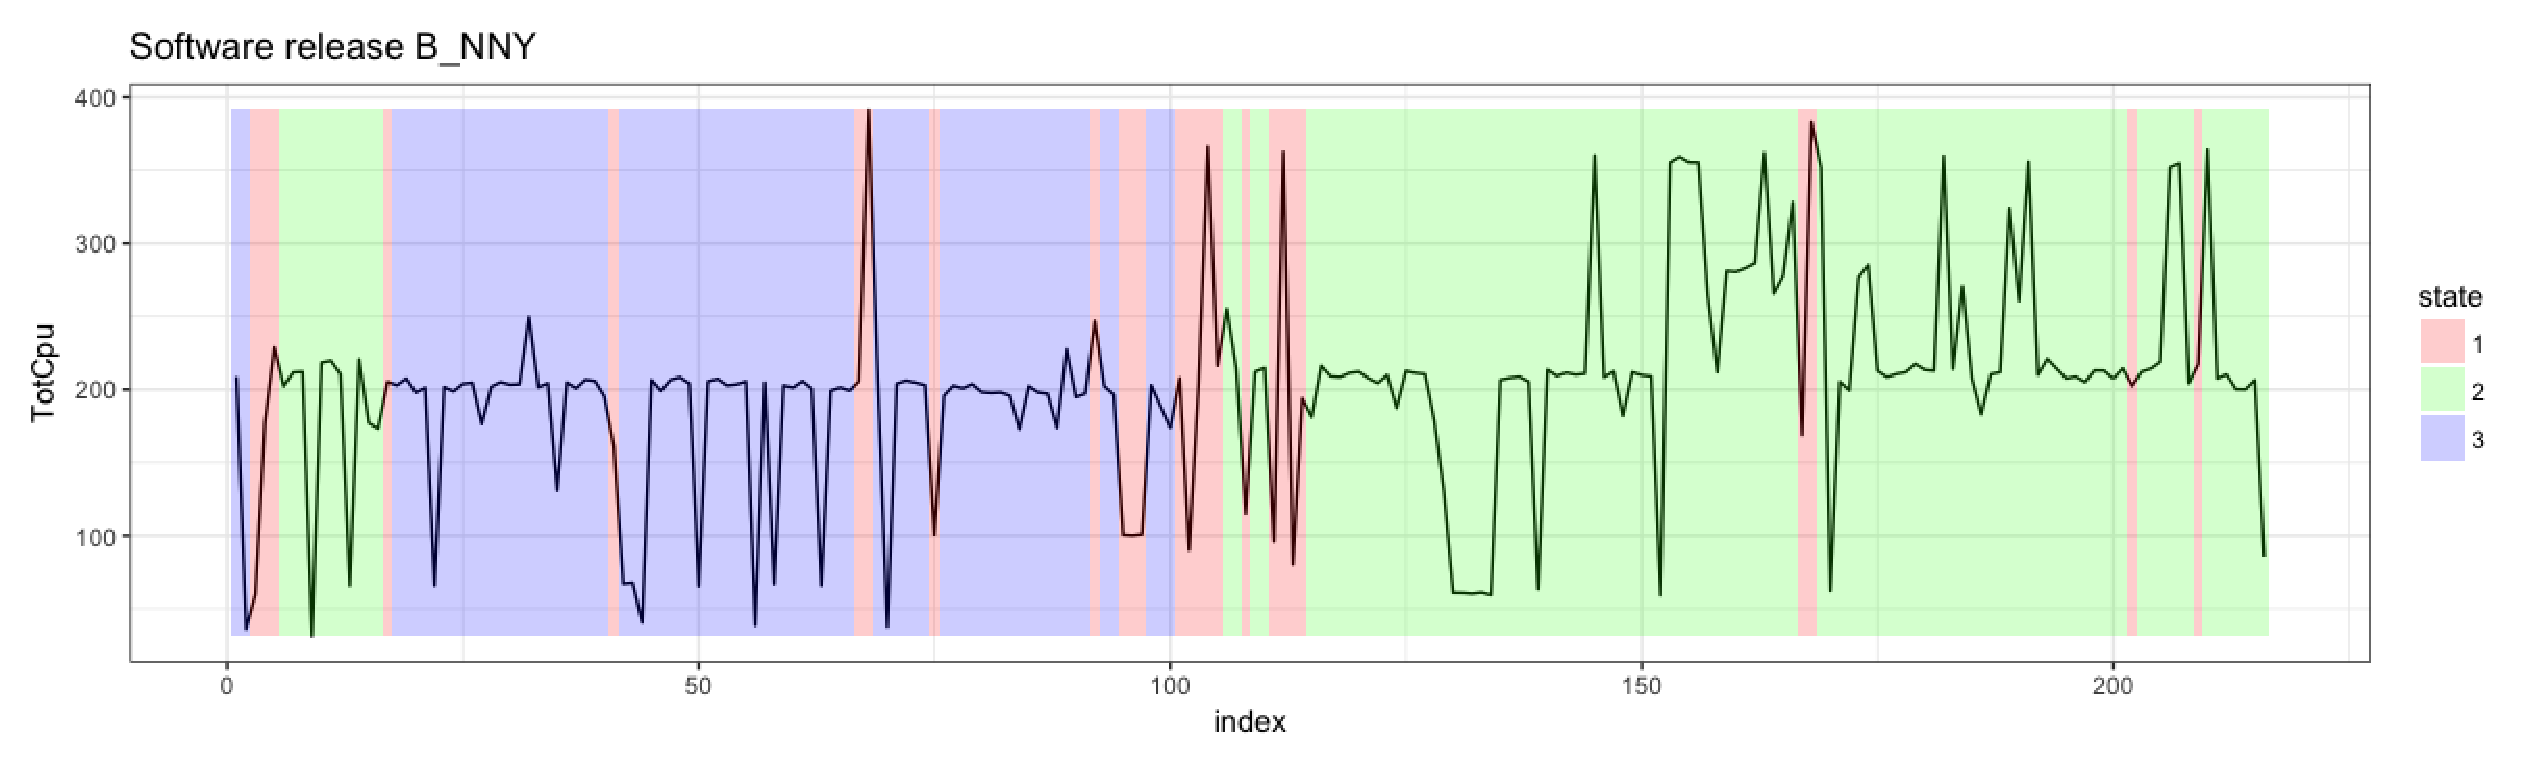
\includegraphics[scale=0.35]{picture/L16B_NNY1}
\par\end{centering}
\caption{The CPU utilization of the software release L16B showing the periods
where the observation is in the specific state. \protect \\
Model 2: DuProdName and Fdd/Tdd are non-switching coefficients.}
\label{L16B_NNY}
\end{figure}




\cleardoublepage{}

\bibliographystyle{apalike}
\bibliography{ThesisTemplate}

\cleardoublepage{}

\lhead[]{Nomenclature}

\rhead[Nomenclature]{}

\printnomenclature[2.5cm]{}
\end{document}
